%
% Programming in Cryptol
% Galois, Inc.
% Levent Erkok, Dylan McNamee, Joseph Kiniry, and others
%

\documentclass[twoside]{book}
% \usepackage{layout}
% \usepackage{diagrams}
\usepackage{amsfonts}
\usepackage{xspace}
\usepackage{url}
\usepackage{subfigure}
\usepackage{graphicx}
\usepackage{lastpage}
\usepackage{makeidx}
\usepackage{longtable}
\usepackage{booktabs}
\usepackage[disable]{todonotes}
\usepackage[myheadings]{fullpage}
\usepackage{verbatim}
%% \usepackage[lighttt]{lmodern}
%% \usepackage[ttscale=1.15]{lmodern}
\usepackage{fancyvrb}
\usepackage{amsmath, amsthm, amssymb}
\usepackage{fancyhdr}
\usepackage{xcolor}
\usepackage{pdfpages}
\usepackage[answerdelayed,lastexercise]{utils/exercise}
\usepackage[bookmarks=true,pagebackref=true,linktocpage=true]{hyperref}
\usepackage[style=list]{utils/glossary}
\usepackage{adjustbox}
%\usepackage[paperwidth=5.5in,paperheight=8.5in]{geometry}
\usepackage{geometry}

% for bound books:
%\setlength{\textwidth}{340pt}
%\setlength{\textheight}{502pt}

\newcommand{\titleline}{Programming in Cryptol}

\hypersetup{%
   pdftitle     = \titleline,
   pdfkeywords  = {Cryptol, Cryptography, Programming},
   pdfauthor    = {Galois, Inc.},
   pdfpagemode  = UseOutlines,
   pdfborder    = 0 0 0
}

\input{utils/Indexes.tex}
\input{utils/GlossaryItems.tex}
\input{utils/trickery.tex}

% fonts
\usepackage{fontspec}
\usepackage{xunicode}
\usepackage{xltxtra}
\defaultfontfeatures{Mapping=tex-text}
\setmainfont[]{Times}
\setsansfont[]{Helvetica}
\setmonofont[Scale=0.85]{Courier}
\usepackage{sectsty}
\allsectionsfont{\sffamily}

\newcommand{\lamex}{\ensuremath{\lambda}-expression\indLamExp}
\newcommand{\lamexs}{\ensuremath{\lambda}-expressions\indLamExp}
\makeatletter
\def\imod#1{\allowbreak\mkern3mu({\operator@font mod}\,\,#1)}
\makeatother

\newcommand{\ticket}[1]{\href{https://www.galois.com/cryptol/ticket/#1}{ticket \##1}}

\newcommand{\advanced}{\begin{center}\framebox{\begin{minipage}{0.95\textwidth}{{\bf
Note:} The material in this section is aimed for the more
advanced reader. It can be skipped on a first reading
without loss of continuity.}\end{minipage}}\end{center}}

\newcommand{\sectionWithAnswers}[2]{%
\AnswerBoxSectionMark{Section \arabic{chapter}.\arabic{section} #1 (p.\pageref{#2})}%
\AnswerBoxExecute{\addcontentsline{toc}{section}{\texorpdfstring{\parbox{2.3em}{\arabic{chapter}.\arabic{section}\ }}{(\arabic{chapter}.\arabic{section})\ }#1}}%
}

\theoremstyle{definition}
\newcommand{\commentout}[1]{}
\DefineVerbatimEnvironment{code}{Verbatim}{}
\renewcommand{\ExerciseHeaderTitle}{\ExerciseTitle}
\renewcommand{\ExerciseHeader}{\textbf{\hspace*{-\parindent}\ExerciseName\ \theExercise.\ }}
\renewcommand{\AnswerHeader}{\textbf{\hspace*{-\parindent}\ExerciseName\ \theExercise.\ }}
\renewcounter{Exercise}[chapter]
\newcommand{\unparagraph}{\paragraph{$\,\,\,$\hspace*{-\parindent}}}

% various little text sections:
\newtheorem*{tip}{Tip}
\newtheorem*{hint}{Hint}
\newtheorem*{nb}{NB}
\newtheorem*{notesThm}{Note}
\newcommand{\note}[1]{\begin{notesThm}{#1}\end{notesThm}}
\newcommand{\lhint}[1]{({\bf Hint:}\ #1)}
\newcommand{\ansref}[1]{{\bf (p.~\pageref{#1})}}
%% \newcommand{\draftdate}{DRAFT of \today}
\setlength{\headsep}{2cm}
\setlength{\headheight}{15.2pt}
\renewcommand{\headrulewidth}{0pt} % no line on top
\renewcommand{\footrulewidth}{.5pt} % line on bottom
\renewcommand{\chaptermark}[1]{\markboth{#1}{}}
\renewcommand{\sectionmark}[1]{\markright{#1}{}}
\newcommand{\changefont}{%
    \fontsize{9}{10}\selectfont
}
\cfoot{}
\fancyfoot[LE,RO]{\changefont{\textsf{\thepage}}}
\fancyfoot[LO,RE]{\changefont{\textsf{\copyright\ 2010--2014, Galois, Inc.}}}
%% \fancyhead[LE]{\fancyplain{}{\textsf{\draftdate}}}
%% \fancyhead[RO]{\fancyplain{}{\textsf{DO NOT DISTRIBUTE!}}}
\fancyhead[RO,LE]{\fancyplain{}{}} %% outer
%\fancyhead[LO,RE]{\fancyplain{}{\textsf{\nouppercase{\rightmark}}}}
\fancyhead[LO,RE]{\fancyplain{}{\textsf{\nouppercase{\rightmark}}}} %% inner
\pagestyle{fancyplain}

\makeglossary
\makeindex

\begin{document}

\title{\Huge{\bf \titleline}}
\author{\\$ $\\$ $\\
        Galois, Inc.\\
        421 SW 6th Ave., Suite 300\\Portland, OR 97204}
\date{
\vspace*{2cm}$ $\\
\includegraphics{utils/galois.jpg}
}

\pagenumbering{roman}

%% \includepdf[pages={1},scale=1.0]{cover/CryptolSmallCover.pdf}
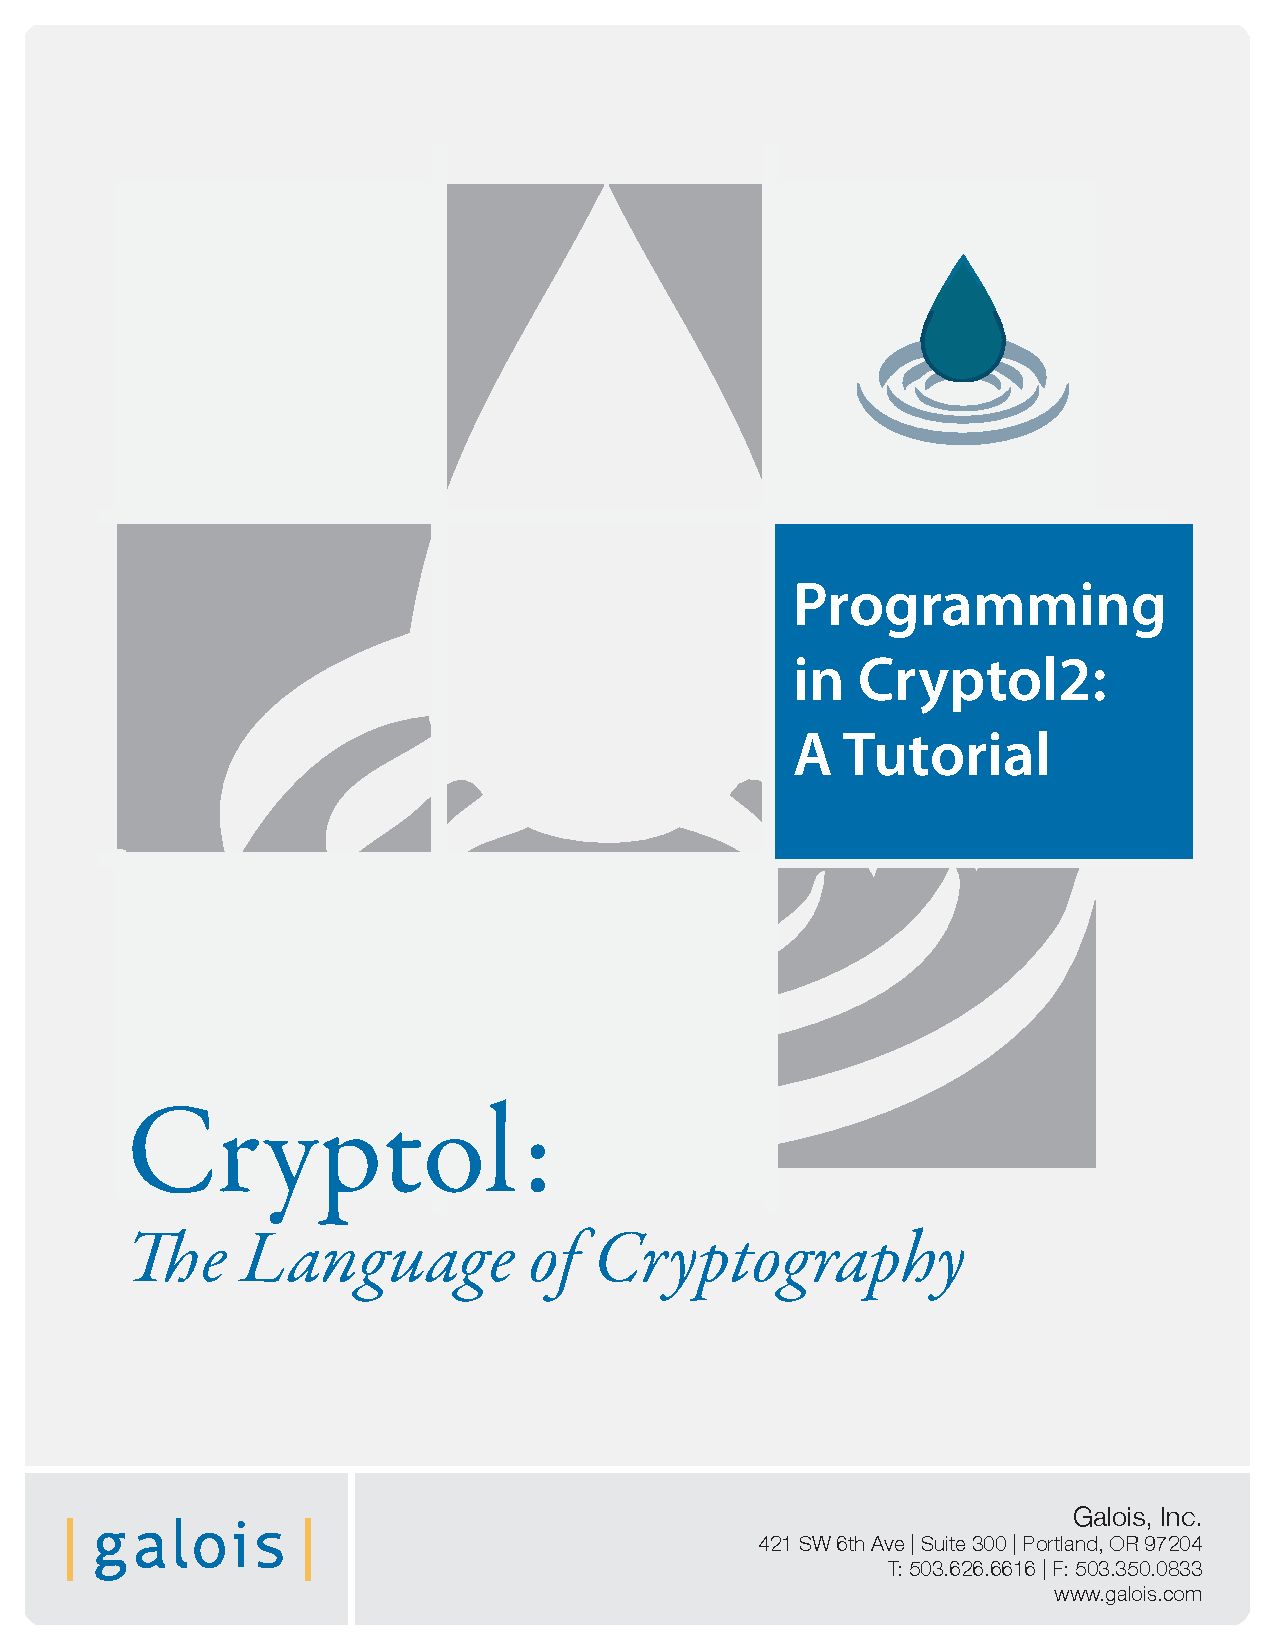
\includepdf[pages={1},scale=1.0]{cover/ProgrammingCryptolCover.pdf}

%\advance\voffset by -26pt
%\setlength{\hoffset}{-26pt}

% for bound-books
% \setlength{\oddsidemargin}{36pt}
% \setlength{\evensidemargin}{-36pt}

% \maketitle
%%
\index{inference|see{type, inference}}
\index{signature|see{type, signature}}
\index{polymorphism|see{type, polymorphism}}
\index{monomorphism|see{type, monomorphism}}
\index{overloading|see{type, overloading}}
\index{undecidable|see{type, undecidable}}
\index{predicates|see{type, predicates}}
\index{defaulting|see{type, defaulting}}
\index{fin@\texttt{fin}|see{type, fin}}
\index{ambiguous constraints|see{type, ambiguous}}
\index{wildcard|see{\texttt{\_} (underscore)}}
\index{lambda expression|see{\ensuremath{\lambda}-expression}}
\index{pdiv@\texttt{pdiv}|see{polynomial, division}}
\index{pmod@\texttt{pmod}|see{polynomial, modulus}}
\index{pmult@\texttt{pmult}|see{polynomial, multiplication}}
\index{000GF28@GF($2^8$)|see{galois field}}

\setlength{\headsep}{24pt}
% \layout

\input{title/Title.tex}
\newpage

\input{preface/Notice.tex}
\newpage

%%%%%% TOC
\tableofcontents

% \includepdf[pages={1}]{cover/Blank.pdf}
\vfill
\eject

\listoftodos
\newpage

%%%%%% Preface
\input{preface/Preface.tex}

\setcounter{page}{1}
\pagenumbering{arabic}

\input{main/todo.tex}

%%%%%% Installation and Tool Use
\input{installation/Install.tex}
\commentout{
\begin{code}
include "../installation/Install.tex";
\end{code}
}

%%%%%% Crash Course
\commentout{
\begin{code}
  module CrashCourse where
\end{code}
}

%#####################################################################
\chapter{A Crash Course in Cryptol}
\label{cha:crash-course-cryptol}

Before we can delve into cryptography, we have to get familiar with
Cryptol.  This chapter provides an introduction to Cryptol, just to
get you started. The exposition is not meant to be comprehensive, but
rather as an overview to give you a feel of the most important tools
available.  If a particular topic appears hard to approach, feel free
to skim it over for future reference.  

A full language reference is beyond the scope of this document at this
time.
% The language features not covered in this document at this time
% include:
% \begin{itemize}
% \item feature one
% \item feature two
% \end{itemize}
% \todo[inline]{2.1: Add list here of language features not yet
%   covered.}

The full grammar for Cryptol is included
in~\autoref{cha:cryptol-grammar}.

%=====================================================================
\section{Basic data types}
\label{sec:basic-data-types}

Cryptol provides four basic data types: bits, sequences, tuples, and
records.  Words (i.e., numbers) are a special case of sequences.  Note
that, aside from bits, all other Cryptol types can be nested as deep
as you like. That is, we can have records of sequences containing
tuples that comprise of other records, etc., giving us a rich
type-system for precisely describing the shapes of data our programs
manipulate.

While Cryptol is statically typed, it uses type inference to supply
unspecified types.  That is, the user does {\em not} have to write the
types of all expressions, they will be automatically inferred by the
type-inference engine.  Of course, in certain contexts the user might
choose to supply a type explicitly.  The notation is simple: we simply
put the expression, followed by {\tt :} and the type. For instance:
\begin{Verbatim}
   12 : [8]
\end{Verbatim}
means the value {\tt 12} has type {\tt [8]}, i.e., it is an 8-bit
word. We shall see other examples of this in the following discussion.

%=====================================================================
\section{Bits: Booleans}
\label{sec:bits}
\sectionWithAnswers{Bits: Booleans}{sec:bits}

The type {\tt Bit}\indTheBitType represents a single bit of
information. There are precisely two values of this type: {\tt
  True}\indTrue and {\tt False}\indFalse. Bit values play an important
role in Cryptol, as we shall see in detail shortly. In particular, the
test expression in an {\tt if-then-else} statement must have the type
{\tt Bit}.  The logical operators {\tt \&\&}\indAnd (and), {\tt
  ||}\indOr (or), {\tt \Verb|^|}\indXOr (xor), and {\tt
  \Verb|~|}\indComplement (complement) provide the basic operators
that act on bit values.

\begin{Exercise}\label{ex:dataBit}
  Type in the following expressions at the Cryptol prompt, and observe
  the output:
\begin{Verbatim}
  True
  false
  False : Bit
  if True && False then 3 else 4
  False || True
  (True && False) ^ True
  ~False
  ~(False || True)
\end{Verbatim}
Remember that Cryptol is case sensitive, and hence {\tt false} is
different from {\tt False}.\indCaseSensitive
\end{Exercise}
\begin{Answer}\ansref{ex:dataBit}
Here is the response from Cryptol, in order:
\begin{small}
\begin{Verbatim}
  True
  [error] at <interactive>:1:1--1:8: Variable `false` was not defined.
  False
  0x4
  True
  True
  True
  False
\end{Verbatim}
\end{small}
\end{Answer}

\begin{tip}
  Cryptol provides extensive command line/tab completion; use
  up/down-arrow to see your previous commands, hit tab to complete
  identifier names, etc.
\end{tip}

%=====================================================================
\section{Words: Numbers}
\label{sec:words}
\sectionWithAnswers{Words: Numbers}{sec:words}

A word is simply a numeric value, corresponding to the usual notion of
numbers.\indTheWordType To match our observation of how cryptographers
use numbers, Cryptol only supports non-negative ($\geq 0$) integer
values (i.e., no floating point or negative numbers).\indFloatingPoint
However, numbers can be arbitrarily large: There is no predefined
maximum that we are limited to.\indArbitraryPrecision By default,
Cryptol prints numbers in base 16. You might find it useful to set the
output base to be 10 while working on the following example. To do so,
use the command:\indSettingBase
\begin{Verbatim}
  :set base=10
\end{Verbatim}
The most common values for this setting are 2 (binary), 8 (octal), 10
(decimal), and 16 (hexadecimal).  Conversely, we can \emph{write}
numbers in these bases in Cryptol programs too:
\begin{Verbatim}
  0b11111011110    // binary
  0o3736           // octal
  2014             // decimal
  0x7de            // hexadecimal
\end{Verbatim}

For printing values in arbitrary bases, Cryptol uses the notation {\tt
  0<base>digits}, where base is the base value and the digits are the
numeric value in that particular base.  E.g., the above value is equal
to \texttt{0<7>5605} and \texttt{0<20>50e}.  One cannot input a value
in a non-standard base.\footnote{Cryptol does not support the input of
  numbers in arbitrary bases---the use of non-standard bases (i.e.,
  beyond base 2, 8, 10, and 16) is vanishingly rare and thus not worth
  the trouble in complicating the Cryptol parser.}

\note{Decimal numbers pose a problem in a bit-precise language like
  Cryptol.  Numbers represented in a base that is a power of two
  unambiguausly specify the number of bits required to store each
  digit.  For example {\tt 0b101} takes three bits to store. A
  hexadecimal digit takes 4 bits to store, so {\tt 0xabc} needs 12
  bits.  On the other hand, in decimal, the number of bits is
  ambiguous.  A decimal digit could require anywhere from 1 to 4 bits
  to represent.  When given a choice, Cryptol assumes the
  \emph{smallest} number of bits required to represent a decimal
  number. This is why Cryptol often prints messages like {\tt Assuming
    a = 3}; the value emitted are the number of bits necessary to
  faithfully represent the decimal value on the corresponding line.}

\todo[inline]{2.1: Make decision about
  \href{https://www.galois.com/cryptol/ticket/217}{ticket \#217} for
  the suppression of bitwidth assumption messages.}
%% If you get tired of these messages, you can suppress them with the
%% \texttt{:set reportAssuming=off} command.  Alternatively, you can
%% help Cryptol avoid from having to assume anything by using binary,
%% octal, or hexadecimal constants exclusively.  Many cryptographic
%% algorithms use decimal for their constants, but it is important to
%% keep track of how many bits they need, so the current behavior was
%% deemed a good compromise.

\begin{Exercise}\label{ex:setBase}
  Experiment with different output bases by issuing {\tt :set
    base=10}, and other base values. Also try writing numbers directly
  in different bases at the command line, such as {\tt 0o1237}.  Feel
  free to try other bases.  What is the hexadecimal version of the
  octal number {\tt 0o7756677263570015}?  Observe that {\tt :base=}
  can be set to anything between 2 and 36. Why does Cryptol stop at
  36?
\end{Exercise}
\begin{Answer}\ansref{ex:setBase}
{\tt 0xfeedfacef00d}.
Allowing base 1 would have resulted in unreadable output, and anything
larger than 36 would have required Cryptol to use unicode for digits
(and would have limited utility). As usual {\tt a} is 10, {\tt b} is
11, \ldots z is 36. Remember that upper and lower case letters denote
the same value, so {\tt a} and {\tt A} both represent 10.
\end{Answer}

\note{We will revisit the notion of numbers in
  Section~\ref{sec:words2}, after we learn about sequences.}

%=====================================================================
\section{Tuples: Heterogeneous collections}
\label{sec:tuple}
\sectionWithAnswers{Tuples: Heterogeneous collections}{sec:tuple}

A tuple is a simple collection of arbitrary ordered values of
arbitrary types, written in parentheses.\indTheTupleType A tuple is at
least a pair; it has at least two elements\footnote{Tuples with zero
  and one element are part of the underlying mathematics of Cryptol's
  tuple theory but are not supported in its concrete syntax because
  doing so unnecessarily complicates the parser and program
  comprehension.}, and can be arbitrarily nested with other types.
Elements are comma separated.  

Two tuples are equal in the standard fashion: if they have the same
arity, their types are pairwise comparable
(see~\autoref{sec:type-classes}), and their values are pairwise
identical.  Note that their types need not be pairwise identical; for
example, consider the expression \texttt{('A', 0) == (65, 0)}.  The
type of the LHS is \texttt{{a} (fin a) => ([8], [a])} while the RHS is
\texttt{{a, b} (a >= 7, fin a, fin b) => ([a], [b])}.

\todo[inline]{2.1: Decide upon the status of
  \href{https://www.galois.com/cryptol/ticket/248}{ticket \#248} wrt
  tuple semantics.  Fundamentally, why do we not support zero and one
  element tuples?}

\begin{Exercise}\label{ex:tup:1}
Try out the following tuples:
\begin{Verbatim}
  (1, 2+4)
  (True, False, True ^ False)
  ((1, 2), False, (3-1, (4, True)))
\end{Verbatim}
\end{Exercise}
\begin{Answer}\ansref{ex:tup:1}
Here are Cryptol's responses:
\begin{Verbatim}
  (1, 6)
  (True, False, True)
  ((1, 2), False, (2, (4, True)))
\end{Verbatim}
\end{Answer}

\todo[inline]{Reflect upon these computed expressions.  What is the
  operational semantics of computation of constant-valued arithmetic
  expressions?  There seems to be differing behavior between
  object-level and type-level expressions, but also differing
  semantics at the object level in different contexts.}

\paragraph*{Projecting values from tuples} Use a {\tt .} followed by
$n$ to project the $n+1$-th component of a tuple.  Nested projection is
not supported at this time.

\begin{Exercise}\label{ex:tup:2}
Try out the following examples:
\begin{Verbatim}
  (1, 2+4).0
  (1, 2+4).1
  ((1, 2), False, (3-1, (4, True))).2
\end{Verbatim}
\todo[inline]{Include a more interesting nested example here once
  \href{https://www.galois.com/cryptol/ticket/220}{ticket \#220} is
  fixed. As in, extract the value True, using ".2.2.2".}  Write a
projection to extract the value {\tt False} from the expression:
\begin{Verbatim}
  ((1, 2), (2, (4, True), 6), False)
\end{Verbatim}
\end{Exercise}
\begin{Answer}\ansref{ex:tup:2}
Here are Cryptol's responses:
\begin{Verbatim}
  Cryptol> (1, 2+4).0
  1
  Cryptol> (1, 2+4).1
  6
  Cryptol> ((1, 2), False, (3-1, (4, True))).2
  (2, (4, True))
\end{Verbatim}
The required expression would be:
\begin{Verbatim}
  ((1, 2), (2, (4, True), 6), False).2
\end{Verbatim}
\end{Answer}

\begin{tip}
  While projections can come in handy, we rarely see them used in
  Cryptol programs. As we shall see later, Cryptol's powerful
  pattern-matching mechanism provides a much nicer and usable
  alternative for extracting parts of tuples and other composite data
  values.
\end{tip}

%=====================================================================
\section{Sequences: Homogeneous collections}
\label{sec:sequences}
\sectionWithAnswers{Sequences: Homogeneous collections}{sec:sequences}

While tuples contain heterogeneous data, sequences are used for
homogeneous collections of values, akin to value arrays in more
traditional languages.  A sequence contains elements of any
\emph{single} type, even sequences themselves, arbitrarily nested.  We
simply write a sequence by enclosing it within square brackets with
comma-separated elements.\indTheSequenceType

\begin{Exercise}\label{ex:seq:1}
Try out the following sequences:
\begin{Verbatim}
  [1, 2]
  [[1, 2, 3], [4, 5, 6], [7, 8, 9]]
\end{Verbatim}
Note how the latter example can be used as the representation of a
$3\times3$ matrix.
\end{Exercise}

\begin{tip}
  The most important thing to remember about a sequence is that its
  elements must be of exactly the same type.
\end{tip}

\begin{Exercise}\label{ex:seq:2}
  Type in the following expressions to Cryptol and observe the
  type-errors:
\begin{Verbatim}
  [True, [True]]
  [[1, 2, 3], [4, 5]]
\end{Verbatim}
\end{Exercise}
\begin{Answer}\ansref{ex:seq:2}
In each case we get a type-error:
\begin{Verbatim}
  Cryptol> [1, True]
  [error] at <interactive>:1:1--1:10:
    Type mismatch:
      Expected type: [?a]
      Inferred type: Bit
  Cryptol> [[1, 2, 3], [4, 5]]
  [error] at <interactive>:1:1--1:20:
    Type mismatch:
      Expected type: [3][?a]
      Inferred type: [2][?b]
\end{Verbatim}
In the first case, we are trying to put a bit ({\tt True}) and a
singleton sequence containing a bit ({\tt [True]}) in the same
sequence, which have different types. In the second case, we are
trying to put two sequences of different lengths into a sequence,
which again breaks the homogeneity requirement.
\end{Answer}

%~~~~~~~~~~~~~~~~~~~~~~~~~~~~~~~~~~~~~~~~~~~~~~~~~~~~~~~~~~~~~~~~~~~~~
\subsection{Enumerations}\indEnum
\label{sec:enumerations}

Cryptol enumerations allow us to write sequences more compactly,
instead of listing the elements individually.  An enumeration is a
means of writing a sequence by providing a (possibly infinite) range.
Cryptol enumerations are not equivalent to mainstream programming
languages' notions of enumeration types, other than both kinds of
constructs guarantee that enumeration elements are distinct.

\begin{Exercise}\label{ex:seq:3}
  Explore various ways of constructing enumerations in Cryptol, by
  using the following expressions:
\begin{Verbatim}
  [1 .. 10]       // increment with step 1
  [1, 3 .. 10]    // increment with step 2 (= 3-1)
  [10, 9 .. 1]    // decrement with step 1 (= 10-9)
  [10, 9 .. 20]   // decrement with step 1 (= 10-9)
  [10, 7 .. 1]    // decrement with step 3 (= 10-7)
  [10, 11 .. 1]   // increment with step 1
\end{Verbatim}
\end{Exercise}
\begin{Answer}\ansref{ex:seq:3}
Here are the responses from Cryptol:
\begin{Verbatim}
  [1, 2, 3, 4, 5, 6, 7, 8, 9, 10]
  [1, 3, 5, 7, 9]
  [10, 9, 8, 7, 6, 5, 4, 3, 2, 1]
  []
  [10, 7, 4, 1]
  []
\end{Verbatim}
Note how {\tt [10, 11 .. 1]} and {\tt [10, 9 .. 20]} give us empty
sequences, since the upper bound is smaller than the lower bound in
the former, and larger in the latter.
\end{Answer}

%~~~~~~~~~~~~~~~~~~~~~~~~~~~~~~~~~~~~~~~~~~~~~~~~~~~~~~~~~~~~~~~~~~~~~
\subsection{Comprehensions}\indComp
\label{sec:comprehensions}

A Cryptol comprehension is a way of programmatically computing the
elements of a new sequence, out of the elements of existing
ones.\indComp  The syntax is reminiscent of the set comprehension
notation from ordinary mathematics, generalized to cover parallel
branches (as explained in the exercises below).  Note that Cryptol
comprehensions are not generalized numeric comprehensions (like
summation, product, maximum, or minimum), though such comprehensions
can certainly be defined using Cryptol comprehensions.

\begin{Exercise}\label{ex:seq:4}
  A comprehension with a single arm is called a {\em cartesian
    comprehension}. We can have one or more components in a cartesian
  comprehension.  Experiment with the following
  expressions:\indComp\indCartesian
\begin{Verbatim}
   [ (x, y) | x <- [1 .. 3], y <- [4, 5] ]
   [ x + y  | x <- [1 .. 3], y <- [] ]
   [ (x + y, z)  | x <- [1, 2], y <- [1], z <- [3, 4] ]
\end{Verbatim}
What is the number of elements in the resulting sequence, with respect
to the sizes of components?

\note{Recall that, when you type the expressions above, you will get
  messages from Cryptol such as {\tt Assuming a = 2}.  This is Cryptol
  letting you know it has decided to use 2 bits to represent, for
  example, the value {\tt 3} in {\tt [1 .. 3]}. This information may
  not seem to matter now but it can be very helpful later
  on.}
\end{Exercise}
\begin{Answer}\ansref{ex:seq:4}
Here are the responses from Cryptol:
\begin{Verbatim}
  [(1, 4) (1, 5) (2, 4) (2, 5) (3, 4) (3, 5)]
  []
  [(2, 3) (2, 4) (3, 3) (3, 4)]
\end{Verbatim}
The size of the result will be the sizes of the components
multiplied. For instance, in the first example, the generator {\tt x
  <- [1 .. 3]} assigns 3 values to {\tt x}, and the generator {\tt y
  <- [4, 5]} assigns 2 values to {\tt y}; and hence the result has
$2\times 3 = 6$ elements.
\end{Answer}

\begin{Exercise}\label{ex:seq:5}\indParallel\indComp
  A comprehension with multiple arms is called a {\em parallel
    comprehension}.  We can have any number of parallel arms. The
  contents of each arm will be {\em zipped} to obtain the results.
  Experiment with the following expressions:
\begin{Verbatim}
   [ (x, y) | x <- [1 .. 3] | y <- [4, 5] ]
   [ x + y  | x <- [1 .. 3] | y <- [] ]
   [ (x + y, z)  | x <- [1, 2] | y <- [1] | z <- [3, 4] ]
\end{Verbatim}
What is the number of elements in the resulting sequence, with respect
to the sizes of the parallel branches?
\end{Exercise}
\begin{Answer}\ansref{ex:seq:5}
Here are the responses from Cryptol:
\begin{Verbatim}
  [(1, 4) (2, 5)]
  []
  [(2, 3)]
\end{Verbatim}
In this case, the size of the result will be the minimum of the
component sizes. For the first example, the generator {\tt x <- [1
  .. 3]} assigns 3 values to {\tt x}, and the generator {\tt y <- [4,
  5]} assigns 2 values to {\tt y}; and hence the result has $\min(2,3)
= 2$ elements.
\end{Answer}

\begin{tip}
  One can mix parallel and cartesian comprehensions, where each
  parallel arm can contain multiple cartesian
  generators, or vice-versa.\indComp\indCartesian\indParallel
\end{tip}

\begin{tip}
  While Cryptol comprehensions \emph{look} like standard mathematical
  comprehensions, one must remember that the codomain of Cryptol
  comprehensions is a sequence type of some kind, \emph{not} a set.
\end{tip}

Comprehensions may be nested.\indNestedComp In this pattern, the
element value expression of the outer nesting is a sequence
comprehension (which may refer to values generated by the outer
generator). The pattern looks like this:
\begin{minipage}{\textwidth}  %% trying to avoid splitting this across pages
\begin{Verbatim}
  [  [ <expr with x & y>  //                   \
       | y <- [1 .. 5]    // inner generator    -- outer elements
     ]                                         /
     | x <- [1 .. 5]      // outer generator
  ]
\end{Verbatim}
\end{minipage}

\begin{Exercise}\label{ex:seq:6}
  Use a nested comprehension to write an expression to produce a
  $3\times3$ matrix (as a sequence of sequences), such that the $ij$th
  entry contains the value {\tt (i, j)}.
\end{Exercise}
\begin{Answer}\ansref{ex:seq:6}
  Here is one way of writing such an expression, layed out in multiple
  lines to show the structure:
\begin{Verbatim}
  [ [ (i, j) | j <- [1 .. 3] ]
     | i <- [1 .. 3]
  ]
  produces:
  [[(1, 1), (1, 2), (1, 3)], 
   [(2, 1), (2, 2), (2, 3)],
   [(3, 1), (3, 2), (3, 3)]]
\end{Verbatim}
The outer comprehension is a comprehension (and hence is nested). In
particular the expression is:
\begin{Verbatim}
     [ (i, j) | j <- [1 .. 3] ]
\end{Verbatim}
You can enter the whole expression in Cryptol all in one line, or
recall that you can put {\tt $\backslash$} at line ends to continue to
the next line.\indLineCont If you are writing such an expression in a
program file, then you can lay it out as shown above or however most
makes sense to you.
\end{Answer}

%~~~~~~~~~~~~~~~~~~~~~~~~~~~~~~~~~~~~~~~~~~~~~~~~~~~~~~~~~~~~~~~~~~~~~
\subsection{Appending and indexing}
\label{sec:appending-indexing}

For sequences, the two basic operations are appending\indAppend ({\tt
  \#}) and selecting\indIndex elements out ({\tt @}, {\tt @@}, {\tt
  !}, and {\tt !!}).  Forward selection operator ({\tt @}), starts
counting from the beginning, while the backward selection
operator\indRIndex ({\tt !}) starts from the end.  Indexing always
starts at zero: That is {\tt xs @ 0} is the first element of {\tt xs},
while {\tt xs ! 0} is the last.  The permutation\indIndexs
versions\indRIndexs ({\tt @@} and {\tt !!}, respectively) allow us to
concisely select multiple elements: they allow us to extract elements
in any order (which makes them very useful for permuting sequences).

\todo[inline]{Cite other languages that express permutations like this?}

\begin{Exercise}\label{ex:seq:7}
Try out the following Cryptol expressions:
\begin{Verbatim}
  [] # [1, 2]
  [1, 2] # []
  [1 .. 5] # [3, 6, 8]
  [0 .. 9] @ 0
  [0 .. 9] @ 5
  [0 .. 9] @ 10
  [0 .. 9] @@ [3, 4]
  [0 .. 9] @@ []
  [0 .. 9] @@ [9, 12]
  [0 .. 9] @@ [9, 8 .. 0]
  [0 .. 9] ! 0
  [0 .. 9] ! 3
  [0 .. 9] !! [3, 6]
  [0 .. 9] !! [0 .. 9]
  [0 .. 9] ! 12
\end{Verbatim}
\end{Exercise}
\begin{Answer}\ansref{ex:seq:7}
Here are Cryptol's responses:
\begin{Verbatim}
  Cryptol> :set warnDefaulting=off
  Cryptol> [] # [1, 2]
  [1, 2]
  Cryptol> [1, 2] # []
  [1, 2]
  Cryptol> [1 .. 5] # [3, 6, 8]
  [1, 2, 3, 4, 5, 3, 6, 8]
  Cryptol> [0 .. 9] @ 0
  0
  Cryptol> [0 .. 9] @ 5
  5
  Cryptol> [0 .. 9] @ 10
  invalid sequence index: 10
  Cryptol> [0 .. 9] @@ [3, 4]
  [3, 4]
  Cryptol> [0 .. 9] @@ []
  []
  Cryptol> [0 .. 9] @@ [9, 12]
  invalid sequence index: 12
  Cryptol> [0 .. 9] @@ [9, 8 .. 0]
  [9, 8, 7, 6, 5, 4, 3, 2, 1, 0]
  Cryptol> [0 .. 9] ! 0
  9
  Cryptol> [0 .. 9] ! 3
  6
  Cryptol> [0 .. 9] !! [3, 6]
  [6, 3]
  Cryptol> [0 .. 9] !! [0 .. 9]
  [9, 8, 7, 6, 5, 4, 3, 2, 1, 0]
  Cryptol> [0 .. 9] ! 12
  invalid sequence index: 12
\end{Verbatim}
\end{Answer}

\begin{Exercise}\label{ex:seq:8}
  The permutation operators ({\tt @@} and {\tt !!}) can be defined
  using sequence comprehensions.  Write an expression that selects the
  even indexed elements out of the sequence {\tt [0 .. 10]} first
  using {\tt @@}, and then using a sequence comprehension.
\end{Exercise}
\begin{Answer}\ansref{ex:seq:8}
Using a permutation operator, we can simply write:
\begin{Verbatim}
  [0 .. 10] @@ [0, 2 .. 10]
\end{Verbatim}
Using a comprehension, we can express the same idea using:
\begin{Verbatim}
  [ [0 .. 10] @ i | i <- [0, 2 .. 10] ]
\end{Verbatim}
Strictly speaking, permutation operations are indeed redundant. 
However, they lead to more concise and easier-to-read expressions.
\end{Answer}

%~~~~~~~~~~~~~~~~~~~~~~~~~~~~~~~~~~~~~~~~~~~~~~~~~~~~~~~~~~~~~~~~~~~~~
\subsection{Finite and infinite sequences}\indFiniteSeq\indInfSeq
\label{sec:finite-infin-sequ}

So far we have only seen finite sequences.  An infinite sequence is one
that has an infinite number of elements, corresponding to
streams.\indStream  Cryptol supports infinite sequences, where the
elements are accessed {\em on-demand}.  This implies that Cryptol will
{\em not} go into an infinite loop just because you have created an
infinite sequence: it will lazily construct the sequence and make its
elements available as demanded by the program.

\begin{Exercise}\label{ex:seq:9}
Try the following infinite enumerations:
\begin{Verbatim}
  [1:[32] ... ]
  [1:[32], 3 ...]
  [1:[32] ...] @ 2000
  [1:[32], 3 ...] @@ [300, 500, 700]
  [100, 102 ...]
\end{Verbatim}
\end{Exercise}
\begin{Answer}\ansref{ex:seq:9}
  When you type in an infinite sequence, Cryptol will only print the
  first 5 elements of it and will indicate that it is an infinite value
  by putting $\ldots$ at the end\footnote{You can change this behavior
    by setting the {\tt infLength} variable, like so: {\tt Cryptol>
      :set infLength=10} will show the first 10 elements of infinite
    sequences}. Here are the responses:
\begin{Verbatim}
  [1, 2, 3, 4, 5, ...]
  [1, 3, 5, 7, 9, ...]
  2001
  [601, 1001, 1401]
  [100, 102, 104, 106, 108, ...]
\end{Verbatim}
\end{Answer}
\note{Note that we are explicitly telling Cryptol to use 32-bit words
  as the elements. The reason for doing so will become clear when we
  study arithmetic shortly.}
\begin{Exercise}\label{ex:seq:10}
  What happens if you use the reverse index operator ({\tt !}) on an
  infinite sequence? Why?
\end{Exercise}
\begin{Answer}\ansref{ex:seq:10}
Here is a simple test case:
\begin{Verbatim}
  Cryptol> ([1 ... ]:[inf][32])!3

[error] at <interactive>:1:1--1:21:
  Unsolved constraint:
    fin inf
      arising from
      use of expression (!)
      at <interactive>:1:19--1:20
\end{Verbatim}
The error message is telling us that we {\em cannot} apply the reverse
index operator ({\tt !}) on an infinite sequence (\texttt{inf}).  This
is a natural consequence of the fact that one can never reach the end
of an infinite sequence to count backwards.  It is important to
emphasize that this is a {\em type-error}, i.e., the user gets this
message at compile time; instead of Cryptol going into an infinite
loop to reach the end of an infinite sequence.
\end{Answer}

%~~~~~~~~~~~~~~~~~~~~~~~~~~~~~~~~~~~~~~~~~~~~~~~~~~~~~~~~~~~~~~~~~~~~~
\subsection{Manipulating sequences} 
\label{sec:manip-sequ}

Sequences are at the heart of Cryptol, and there are a number of
built-in functions for manipulating them in various ways.  It is
worthwhile to try the following exercises to gain basic familiarity
with the basic operations.

\begin{Exercise}\label{ex:seq:11}
Try the following expressions:\indTake\indDrop\indSplitBy\indGroup\indJoin\indTranspose
\begin{Verbatim}
  take`{3} [1 .. 12]
  drop`{3} [1 .. 12]
  split`{3} [1 .. 12]
  groupBy`{3} [1 .. 12]
  join [[1 .. 4], [5 .. 8], [9 .. 12]]
  join [[1, 2, 3], [4, 5, 6], [7, 8, 9], [10, 11, 12]]
  transpose [[1, 2, 3, 4], [5, 6, 7, 8]]
  transpose [[1, 2, 3], [4, 5, 6], [7, 8, 9]]
\end{Verbatim}
And for fun, think about what these should produce:
\begin{Verbatim}
  join [1,1]
  transpose [1,2]
\end{Verbatim}
\end{Exercise}
\begin{Answer}\ansref{ex:seq:11}
Here are Cryptol's responses:
\begin{Verbatim}
  Cryptol> take`{3} [1 .. 12]
  [1, 2, 3]
  Cryptol> drop`{3} [1 .. 12]
  [4, 5, 6, 7, 8, 9, 10, 11, 12]
  Cryptol> split`{3}[1 .. 12]
  [[1, 2, 3, 4], [5, 6, 7, 8], [9, 10, 11, 12]]
  Cryptol> groupBy`{3} [1 .. 12]
  [[1, 2, 3], [4, 5, 6], [7, 8, 9], [10, 11, 12]]
  Cryptol> join [[1 .. 4], [5 .. 8], [9 .. 12]]
  [1, 2, 3, 4, 5, 6, 7, 8, 9, 10, 11, 12]
  Cryptol> join [[1, 2, 3], [4, 5, 6], [7, 8, 9], [10, 11, 12]]
  [1, 2, 3, 4, 5, 6, 7, 8, 9, 10, 11, 12]
  Cryptol> transpose [[1, 2, 3, 4], [5, 6, 7, 8]]
  [[1, 5], [2, 6], [3, 7], [4, 8]]
  Cryptol> transpose [[1, 2, 3], [4, 5, 6], [7, 8, 9]]
  [[1, 4, 7], [2, 5, 8], [3, 6, 9]]
\end{Verbatim}
\todo[inline]{Add discussion about join[1,1] and transpose [1,2].}
\todo[inline]{Why is isn't join in the prelude?!}
\end{Answer}

\begin{Exercise}\label{ex:seq:12}
  Based on your intuitions from the previous exercise, derive laws
  between the following pairs of functions: {\tt take} and {\tt drop};
  {\tt join} and {\tt split}; {\tt join} and {\tt groupBy}; {\tt
    split} and {\tt groupBy} and {\tt transpose} and itself.  For
  instance, {\tt take} and {\tt drop} satisfy the following
  equality:\indTake\indDrop\indJoin\indSplitBy\indGroup\indTranspose
\begin{Verbatim}
   (take`{n} xs) # (drop`{n} xs) == xs
\end{Verbatim}
whenever {\tt n} is between {\tt 0} and the length of the sequence
{\tt xs}. Note that there might be multiple laws these functions
satisfy.
\end{Exercise}
\begin{Answer}\ansref{ex:seq:12}
  The following equalities are the simplest
  candidates:\indJoin\indSplitBy\indGroup\indTranspose
\begin{Verbatim}
  join (split`{parts=n} xs) == xs
  join (groupBy`{each=n} xs) == xs
  split`{parts=n} xs == groupBy`{each=m} xs
  transpose (transpose xs) == xs
\end{Verbatim}
In the first two equalities {\tt n} must be a divisor of the length of
the sequence {\tt xs}.  In the third equation, {\tt n} $\times$ {\tt m}
must equal the length of the sequence {\tt xs}.
\todo[inline]{These are theorems that should be part of the prelude!}
\end{Answer}

\begin{Exercise}\label{ex:seq:13}
What is the relationship between the append operator {\tt \#} and {\tt
  join}?\indAppend\indJoin
\end{Exercise}
\begin{Answer}\ansref{ex:seq:13}
Append ({\tt \#})\indAppend\indJoin joins two sequences of arbitrary
length, while {\tt join} appends a sequence of equal length
sequences. In particular, the equality:
\begin{Verbatim}
   join [xs0, xs1, xs2, .. xsN] = xs0 # xs1 # xs2 ... # xsN
\end{Verbatim}
holds for all equal length sequences {\tt xs0}, {\tt xs1}, $\ldots$,
{\tt xsN}.
\end{Answer}

\paragraph*{Type-directed splits} We have studied the functions {\tt
  groupBy}\indGroup and {\tt splitBy}\indSplit above.  Cryptol also
provides a function {\tt split}\indSplit that can split a sequence
into any number of equal-length segments.  A common way to use {\tt
  split} is to be explicit about the type of its result, instead of
passing arguments as we did above with {\tt splitBy} and {\tt
  groupBy}.
\begin{Verbatim}
  Cryptol> split [1..12] : [1][12][8]
  [[1, 2, 3, 4, 5, 6, 7, 8, 9, 10, 11, 12]]
  Cryptol> split [1..12] : [2][6][8]
  [[1, 2, 3, 4, 5, 6], [7, 8, 9, 10, 11, 12]]
  Cryptol> split [1..12] : [3][4][8]
  [[1, 2, 3, 4], [5, 6, 7, 8], [9, 10, 11, 12]]
\end{Verbatim}
Here is what happens if we do {\em not} give an explicit signature on
the result:\indSignature
\begin{Verbatim}
  Cryptol> split [1..12]
  <polymorphic value>
  Cryptol> :t split [1..12]
  split [1 .. 12] : {a, b, c} (a >= 4, fin a, fin c,
                              12 == b * c) => [b][c][a]
\end{Verbatim}
%% cryptol 1 said: : {a b c} (fin c,c >= 4,a*b == 12) => [a][b][c]

A complex type signature like this one first defines a set of type
variables {\tt \Verb|{a, b, c}|}, a set of constraints on those
variables {\tt \Verb|(a >= 4, fin a, fin c, 12 == b * c)|}, a {\tt =>}
and finally the shape description.  In this case, Cryptol's {\tt
  [b][c][a]} is telling us that the result will be a sequence of {\tt
  b} things, each of which is a sequence of {\tt c} things, each of
which is a word of size {\tt a}. The type constraints tell us that
{\tt a} is at least 4, because the maximum element of the sequence is 12,
and it takes at least 4 bits to represent the value 12.  The
constraints are that {\tt b * c == 12}, which means we should
completely cover the entire input, and that the lengths {\tt a} and
{\tt c} need to be finite.  As you can see, {\tt split} is a very
powerful function. The flexibility afforded by {\tt split} comes in
very handy in Cryptol.  We shall see one example of its usage later in
Section~\ref{sec:scytale}.

\begin{Exercise}\label{ex:split:0}
  With a sequence of length 12, as in the above example, there are
  precisely 6 ways of splitting it: 1--12, 2--6, 3--4, 4--3, 6--2, and
  12--1. We have seen the first three splits above. Write the
  expressions corresponding to the latter 3.\indSplit
\end{Exercise}
\begin{Answer}\ansref{ex:split:0}
Here they are:\indSplit
\begin{Verbatim}
  Cryptol> split [1..12] : [4][3][8]
  [[1, 2, 3], [4, 5, 6], [7, 8, 9], [10, 11, 12]]
  Cryptol> split [1..12] : [6][2][8]
  [[1, 2], [3, 4], [5, 6], [7, 8], [9, 10], [11, 12]]
  Cryptol> split [1..12] : [12][1][8]
  [[1], [2], [3], [4], [5], [6], [7], [8], [9], [10], [11], [12]]
\end{Verbatim}
\end{Answer}

\begin{Exercise}\label{ex:split:1}
  What happens when you type {\tt split [1 .. 12] :
    [5][2][8]}?\indSplit
\end{Exercise}
\begin{Answer}\ansref{ex:split:1}
Cryptol will issue a type error:\indSplit
\begin{Verbatim}
  Cryptol> split [1..12] : [5][2][8]
  Unsolved constraint:
    1 + (12 - 1) == 5 * 2
      arising from
      matching types
      at <interactive>:1:1--1:16
\end{Verbatim}
Cryptol is telling us that we have requested 10 elements in the final
result (5*2), but the input has 12.
\end{Answer}

\begin{Exercise}\label{ex:split:2}
  Write a {\tt split} expression to turn the sequence {\tt [1 .. 120]
    : [120][8]} into a nested sequence with type {\tt [3][4][10][8]},
  keeping the elements in the same order.\indSplit \lhint{Use nested
    comprehensions.}  \indComp
\end{Exercise}
\begin{Answer}\ansref{ex:split:2}
  We can split\indSplit 120 elements first into 3--40, splitting each
  of the the elements ({\tt level1} below) into 4--10. A nested
  comprehension fits the bill:\indComp
\begin{Verbatim}
  [ split level1 : [4][10][8]
  | level1 <- split ([1 .. 120] : [120][8]) : [3][40][8]
  ]
\end{Verbatim}
(Note again that you can enter the above in the command line all in
one line, or by putting the line continuation character {\tt
  $\backslash$} at the end of the first two lines.)\indLineCont
\end{Answer}

%~~~~~~~~~~~~~~~~~~~~~~~~~~~~~~~~~~~~~~~~~~~~~~~~~~~~~~~~~~~~~~~~~~~~~
\subsection{Shifts and rotates} 
\label{sec:shifts-rotates}

Common operations on sequences include shifting and rotating them.
Cryptol supports both versions with left/right
variants.\indShiftLeft\indShiftRight\indRotLeft\indRotRight
\begin{Exercise}\label{ex:seq:14}
Experiment with the following expressions:
\begin{Verbatim}
   [1, 2, 3, 4, 5] >> 2
   [1, 2, 3, 4, 5] >> 10
   [1, 2, 3, 4, 5] << 2
   [1, 2, 3, 4, 5] << 10
   [1, 2, 3, 4, 5] >>> 2
   [1, 2, 3, 4, 5] >>> 10
   [1, 2, 3, 4, 5] <<< 2
   [1, 2, 3, 4, 5] <<< 10
\end{Verbatim}
\noindent Notice that shifting/rotating always returns a sequence
precisely the same size as the original.
\end{Exercise}
\begin{Answer}\ansref{ex:seq:14}
Here are Cryptol's responses:
\begin{Verbatim}
  [0, 0, 1, 2, 3]
  [0, 0, 0, 0, 0]
  [3, 4, 5, 0, 0]
  [0, 0, 0, 0, 0]
  [4, 5, 1, 2, 3]
  [1, 2, 3, 4, 5]
  [3, 4, 5, 1, 2]
  [1, 2, 3, 4, 5]
\end{Verbatim}
\todo[inline]{Reflections on this exercise?}
\end{Answer}
\begin{Exercise}\label{ex:seq:15}
  Let {\tt xs} be a sequence of length $n$. What is the result of
  rotating {\tt xs} left or right by a multiple of $n$?
\end{Exercise}
\begin{Answer}\ansref{ex:seq:15}
  Rotating (left or right) by a multiple of the size of a sequence
  will leave it unchanged.
\end{Answer}

%=====================================================================
\section{Words revisited}
\label{sec:words2}
\sectionWithAnswers{Words revisited}{sec:words2}

In Section~\ref{sec:words} we have introduced numbers as a distinct
value type in Cryptol. In fact, a number in Cryptol is nothing but a
finite sequence of bits, so words are not a separate type. For
instance, the literal expression {\tt 42} is precisely the same as the
bit-sequence corresponding to {\tt [True, False, True, False, True,
  False]}.\indTheWordType

\begin{Exercise}\label{ex:words:0}
  Explain why {\tt 42} is the same as {\tt [True, False, True, False,
    True, False]}.  Is Cryptol little-endian, or
  big-endian?\indEndianness
\end{Exercise}
\begin{Answer}\ansref{ex:words:0}
  Cryptol is big-endian,\indEndianness meaning that the
  most-significant-bit comes first. In the sequence {\tt [True, False,
    True, False, True, False]}, the first element corresponds to the
  most-significant-digit, i.e., $2^5$, the next element corresponds to
  the coefficient of $2^4$, etc.  A {\tt False} bit yields a
  coefficient of $0$ and a {\tt True} bit gives $1$. Hence, we have:
$$1\times2^5 + 0\times2^4 + 1\times2^3 + 0\times2^2 + 1\times2^1 + 0\times2^0 = 32 + 0 + 8 + 0 + 2 + 0 = 42$$
\end{Answer}

\begin{Exercise}\label{ex:words:1}
  Try out the following words: \lhint{It might help to use {\tt :set
      base=2} to see the bit patterns.}\indSettingBase
\begin{Verbatim}
  12
  12 # [False]
  [False, False] # 12
  [True, False] # 12
  12 # [False, True]
  32
  12 # 32
  [True, False, True, False, True, False] == 42
\end{Verbatim}
\end{Exercise}
\begin{Answer}\ansref{ex:words:1}
  After issuing {\tt :set base=2}, here are Cryptol's
  responses:\indSettingBase
\begin{Verbatim}
  0b1100
  0b11000
  0b1100
  0b101100
  0b110001
  0b100000
  0b1100100000
  True
\end{Verbatim}
\end{Answer}

\begin{Exercise}\label{ex:words:2}
  What is the type of {\tt 0}?  Use the {\tt :t} command to find this
  out.  (Type {\tt :t 0} at the prompt.\indSettingType) Are there any
  other elements of this type? What are the elements of the type {\tt
    [2]}?
\end{Exercise}
\begin{Answer}\ansref{ex:words:2}
{\tt 0} has the type {\tt \Verb+{a} [a]+}.
Incidentally, {\tt 0} is the only value that inhabits this type. The
type {\tt [2]} is precisely inhabited by the elements {\tt 0, 1, 2,}
and {\tt 3}.
\todo[inline]{Reflect upon the fact that zero has no length component.}
\end{Answer}

\paragraph*{Defaulting and explicit types}\indDefaulting Top level
polymorphic constants in a Cryptol program are subject to
{\em defaulting}, meaning that Cryptol will use the fewest number of
bits necessary to represent them. Users can override this by giving an
explicit type signature.\indSignature

\begin{Exercise}\label{ex:words:3}
  \todo[inline]{\href{https://www.galois.com/cryptol/ticket/83}{Ticket \#83}
    must be addressed before we can include the text: ``For this
    exercise, first issue {\tt :set +t} command...''.}  Try the
  following expressions:
\begin{Verbatim}
  :t 42
  :t 42 : [9]
  :t 42 : [3]
\end{Verbatim}
Can you jam more bits in a word than is potentially possible in
Cryptol?  Compare this behavior to a typical C expression: {\tt (char)
  9999}.
\end{Exercise}
\begin{Answer}\ansref{ex:words:3}
  The number 42 needs at least 6 bits to represent; hence the last
  expression fails. Note how type-inference helps, as users can give
  type annotations only when they need to be more specific.  Unlike
  the C example, Cryptol will statically make sure that there will not
  be any overflow.
\end{Answer}

\begin{Exercise}\label{ex:words:4}
Since words are sequences, the sequence functions from
Exercise~\ref{sec:sequences}--\ref{ex:seq:11} apply to words as well. Try out
the following examples and explain the outputs you
observe:\indTake\indDrop\indSplit\indGroup
\begin{Verbatim}
  take`{3} 0xFF
  take`{3} (12:[6])
  drop`{3} (12:[6])
  split`{3} (12:[6])
  groupBy`{3} (12:[6])
\end{Verbatim}
\end{Exercise}
\noindent Recall that the notation {\tt 12:[6]} means the constant 12
with the type precisely 6-bits wide.
\begin{Answer}\ansref{ex:words:4}
  Remember that Cryptol is big-endian\indEndianness and hence {\tt
    12:[6]} is precisely {\tt [False, False, True, True, False,
    False]}.  Here are Cryptol's responses:\indTake
\begin{Verbatim}
  Cryptol> take`{3} 0xFF
  7
  Cryptol> take`{3} (12:[6])
  1
  Cryptol> drop`{3} (12:[6])
  4
  Cryptol> split`{3} (12:[6])
  [0, 3, 0]
  Cryptol> groupBy`{3} (12:[6])
  [1, 4]
\end{Verbatim}
For instance, the expression {\tt take`\{3\} (12:[6])} evaluates as follows:
\begin{Verbatim}
  take`{3} (12:[6])
    = take (3, [False, False, True, True, False, False])
    = [False, False, True]
    = 1
\end{Verbatim}
Follow similar lines of reasoning to justify the results for the
remaining expressions.
\end{Answer}
\begin{Exercise}\label{ex:words:5}
  Try Exercise~\ref{ex:words:4}, this time with the constant {\tt
    12:[12]}. Do any of the results change? Why?
\end{Exercise}
\begin{Answer}\ansref{ex:words:5}
  Because of the leading zeros in {\tt 12:[12]}, they all produce
  different results:\indTake\indDrop\indSplit\indGroup
\begin{Verbatim}
  Cryptol> take`{3} (12:[12])
  0
  Cryptol> drop`{3} (12:[12])
  12
  Cryptol> split`{3} (12:[12])
  [0, 0, 12]
  Cryptol> groupBy`{3} (12:[12])
  [0, 0, 1, 4]
\end{Verbatim}
We will show the evaluation steps for {\tt groupBy} here, and urge the
reader to do the same for {\tt splitBy}:
\begin{Verbatim}
  groupBy`{3} (12:[12])
    = groupBy`{3} [False, False, False, False, False, False, 
                   False, False, True, True, False, False]
    = [[False, False, False], [False, False, False] 
       [False, False, True], [True, False, False]]
    = [0, 0, 1, 4]
\end{Verbatim}
\end{Answer}

\paragraph*{Shifts and rotates on words} Consider what happens if we
shift a word, say {\tt 12:[6]} by one to the right:
\indShiftLeft\indShiftRight\indRotLeft\indRotRight
\begin{Verbatim}
  (12:[6]) >> 1
    = [False, False, True, True, False, False] >> 1
    = [False, False, False, True, True, False]
    = 6 
\end{Verbatim}
That is shifting-right by one effectively divides the word by 2. This
is due to Cryptol's ``big-endian'' representation of
numbers\footnote{This is a significant change from Cryptol version 1,
  which interpreted the leftmost element of a sequence as the
  lowest-ordered bit (and thus shifting right was multiplying by 2,
  and shifting left was dividing by 2). The way it is handled now
  matches the traditional
  interpretation.}.\indRotLeft\indRotRight\indShiftLeft\indShiftRight

\begin{Exercise}\label{ex:words:6}
Try the following examples of shifting/rotating words:
\begin{Verbatim}
  (12:[8]) >> 2
  (12:[8]) << 2
\end{Verbatim}
\end{Exercise}
\begin{Answer}\ansref{ex:words:6}
Here are Cryptol's responses:
\begin{Verbatim}
  3
  48
\end{Verbatim}
\todo[inline]{Reflect upon these responses.}
\end{Answer}

\todo[inline]{2.0: This is \textbf{NOT} architecture endianness; we
  need a better discussion here.  Dylan will do some code-diving on
  Cryptol version 1.}

\paragraph*{Little-endian vs Big-endian} The discussion of endianness
comes up often in computer science, with no clear
winner.\indEndianness Since Cryptol allows indexing from the beginning
or the end of a (finite) sequence, you can access the 0th
(least-significant) bit of a sequence $k$ with $k$!0, the 1st bit with
$k$!1, and so on.\indIndex

%=====================================================================
\section{Characters and strings}
\label{sec:charstring}

Strictly speaking Cryptol does {\em not} have characters and strings
as a separate type. However, Cryptol does allow characters in
programs, which simply correspond to their ASCII
equivalents. Similarly, strings are merely sequences of characters,
i.e., sequences of words.\indTheStringType\indTheCharType The
following examples illustrate:
\begin{Verbatim}
  Cryptol> :set base=10
  Cryptol> :set ascii=off
  Cryptol> 'A'
  65
  Cryptol> "ABC"
  [65, 66, 67]
  Cryptol> :set ascii=on
  Cryptol> "ABC"
  "ABC"
  Cryptol> :set ascii=off
  Cryptol> ['A' .. 'Z']
  [65, 66, 67, 68, 69, 70, 71, 72, 73, 74, 75, 76, 77, 78, 79, 
       80, 81, 82, 83, 84, 85, 86, 87, 88, 89, 90]
  Cryptol> :set ascii=on
  Cryptol> ['A' .. 'Z']
  "ABCDEFGHIJKLMNOPQRSTUVWXYZ"
\end{Verbatim}
\note{This is the reason why we have to use the {\tt :set ascii=on}
  command to print ASCII strings.  Otherwise, Cryptol will not have
  enough information to tell numbers from
  characters.\indSettingASCII\indCmdPrint}

\noindent Since characters are simply 8-bit words, you can do word
operations on them; including arithmetic:
\begin{Verbatim}
  Cryptol> 'C' - 'A'
  2
\end{Verbatim}

%=====================================================================
\section{Records: Named collections}
\label{sec:records}
\sectionWithAnswers{Records: Named collections}{sec:records}

In Cryptol, records are simply collections of named fields. In this
sense, they are very similar to tuples (Section~\ref{sec:tuple}),
which can be thought of records without field names\footnote{In fact,
  the fields of a tuple {\it can} be accessed via the dot-notation,
  with their names being their 0-indexed position in the tuple. So
  {\tt (1,2).1 == 2}.}. Like a tuple, the fields of a record can be of
any type.  We construct records by listing the fields inside
curly-braces, separated by commas.  We project fields out of a record
with the usual dot-notation.  Note that the order of fields in a
record is immaterial.\indTheRecordType\indTheTupleType

Record equality is defined in the standard fashion.  Two records are
equal if they have the same number of fields, if their field names are
identical, if identically named fields are of comparable types and
have equal values.

\begin{Exercise}\label{ex:record:1}
Type in the following expressions and observe the output:
\begin{Verbatim}
  {xCoord = 12:[32], yCoord = 21:[32]}
  {xCoord = 12:[32], yCoord = 21:[32]}.yCoord
  {name = "Cryptol", address = "Galois"}
  {name = "Cryptol", address = "Galois"}.address
  {name = "test", coords = {xCoord = 3:[32], yCoord = 5:[32]}}
  {name = "test", coords = {xCoord = 3:[32], \
                            yCoord = 5:[32]}}.coords.yCoord
  {x=True, y=False} == {y=False, x=True}
\end{Verbatim}
\noindent You might find the command {\tt :set
  ascii=on}\indSettingASCII useful in viewing the output.
\end{Exercise}
\begin{Answer}\ansref{ex:record:1}
Here are Cryptol's responses:
\begin{small}
\begin{Verbatim}
  Cryptol> {xCoord = 12:[32], yCoord = 21:[32]}
  {xCoord = 12, yCoord = 21}
  Cryptol> {xCoord = 12:[32], yCoord = 21:[32]}.yCoord
  21
  Cryptol> {name = "Cryptol", address = "Galois"}
  {name = "Cryptol", address = "Galois"}
  Cryptol> {name = "Cryptol", address = "Galois"}.address
  "Galois"
  Cryptol> {name = "test", coords = {xCoord = 3:[32], yCoord = 5:[32]}}
  {name = "test", coords = {xCoord = 3, yCoord = 5}}
  Cryptol> {name = "test", coords = {xCoord = 3:[32], \
                                   yCoord = 5:[32]}}.coords.yCoord
  5
  Cryptol> {x=True, y=False} == {y=False, x=True}
  True
\end{Verbatim}
\end{small}
\end{Answer}

\note{In larger Cryptol programs, records provide quite powerful
  abstraction mechanisms.  In particular, record fields can contain
  polymorphic fields themselves, extracted and used at different types
  in the same expression. However, we will not need that level of
  functionality in our current study.}

%=====================================================================
\section{\texorpdfstring{The {\tt zero}}{The zero}}
\label{sec:zero}
\sectionWithAnswers{\texorpdfstring{The {\tt zero}}{The zero}}{sec:zero}

Before proceeding further, we have to take a detour and talk briefly
about one of the most useful values in Cryptol: {\tt zero}.\indZero
The value {\tt zero} inhabits every type in Cryptol, and stands for
the value that consists of all {\tt False}\indFalse bits. The
following examples should illustrate the idea:
\begin{Verbatim}
  Cryptol> zero : Bit
  False
  Cryptol> zero : [8]
  0
  Cryptol> zero : ([8], Bit)
  (0, False)
  Cryptol> zero : [8][3]
  [0, 0, 0, 0, 0, 0, 0, 0]
  Cryptol> zero : [3](Bit, [4])
  [(False, 0), (False, 0), (False, 0)]
  Cryptol> zero : {xCoord : [12], yCoord : [5]}
  {xCoord=0, yCoord=0}
\end{Verbatim}

\noindent On the other extreme, the value {\tt zero} combined with the
complement operator {\tt \Verb|~|}\indComplement gives us values that
consist of all all {\tt True}\indTrue bits:
\begin{Verbatim}
  Cryptol> ~zero : Bit
  True
  Cryptol> ~zero : [8]
  255
  Cryptol> ~zero : ([8], Bit)
  (255, True)
  Cryptol> ~zero : [8][3]
  [7, 7, 7, 7, 7, 7, 7, 7]
  Cryptol> ~zero : [3](Bit, [4])
  [(True, 15), (True, 15), (True, 15)]
  Cryptol> ~zero : {xCoord : [12], yCoord : [5]}
  {xCoord=4095, yCoord=31}
\end{Verbatim}

\begin{Exercise}\label{ex:zero:0}
  We said that {\tt zero} inhabits all types in Cryptol. This also
  includes functions. What do you think the appropriate {\tt zero}
  value for a function would be?  Try out the following examples:
\begin{Verbatim}
   (zero : ([8] -> [3])) 5
   (zero : Bit -> {xCoord : [12], yCoord : [5]}) True
\end{Verbatim}
\end{Exercise}
\begin{Answer}\ansref{ex:zero:0}
Here are Cryptol's responses:\indZero
\begin{Verbatim}
  Cryptol> (zero : ([8] -> [3])) 5
  0
  Cryptol> (zero : Bit -> {xCoord : [12], yCoord : [5]}) True
  {xCoord=0, yCoord=0}
\end{Verbatim}
The {\tt zero} function returns {\tt 0}, ignoring its argument.
\end{Answer}

%=====================================================================
\section{Arithmetic}
\label{sec:arithmetic}
\sectionWithAnswers{Arithmetic}{sec:arithmetic}

Cryptol supports the usual binary arithmetic operators {\tt +}, {\tt
  -}, {\tt *}, {\tt \Verb|^^|} (exponentiate), {\tt /} (integer
division), {\tt \%} (integer modulus), along with \emph{ceiling}
logarithm base 2 {\tt lg2} and binary {\tt min} and {\tt max}.

The important thing to remember is that all arithmetic in Cryptol is
modular,\indModular with respect to the underlying word size.  As a
consequence, there is no such thing as an overflow/underflow in
Cryptol, as the result will be always guaranteed to fit in the
resulting word size.  While this is very handy for most applications of
Cryptol, it requires some care if overflow has to be treated
explicitly.\indOverflow\indUnderflow\indPlus\indMinus\indTimes\indDiv\indMod\indLg\indMin\indMax\indExponentiate

\begin{Exercise}\label{ex:arith:1}
What is the value of {\tt 1+1}? Surprised?
\end{Exercise}
\begin{Answer}\ansref{ex:arith:1}
  Since {\tt 1} requires only 1-bit to represent, the result also has
  1-bits. In other words, the arithmetic is done modulo $2^1 =
  2$. Therefore, {\tt 1+1 = 0}.
\end{Answer}

\begin{Exercise}\label{ex:arith:2}
What is the value of {\tt 1+(1:[8])}? Why?
\end{Exercise}
\begin{Answer}\ansref{ex:arith:2}
  Now we have 8-bits to work with, so the result is {\tt 2}. Since we
  have 8-bits to work with, overflow will not happen until we get a
  sum that is at least 256.
\end{Answer}

\begin{Exercise}\label{ex:arith:3}
What is the value of {\tt 3 - 5}? How about {\tt (3 - 5) : [8]}?
\end{Exercise}
\begin{Answer}\ansref{ex:arith:3}
  Recall from Section~\ref{sec:words} that there are no negative
  numbers in Cryptol. The values {\tt 3} and {\tt 5} can be
  represented in 3 bits, so Cryptol uses 3-bits to represent the
  result, so the arithmetic is done modulo $2^3=8$. Hence, the result
  is {\tt 6}.  In the second expression, we have 8-bits to work with,
  so the modulus is $2^8 = 256$; so the subtraction results in {\tt
    254} (or {\tt 0xfe}).
\end{Answer}

\note{Cryptol supports subtraction both as a binary operator, and as a
  unary operator. When used in a unary fashion (a.k.a., unary
  minus),\indUnaryMinus it simply means subtraction from {\tt 0}. For
  instance, {\tt -5} precisely means {\tt 0-5}, and is subject to the
  usual modular arithmetic rules.}\indModular\indMinus

\begin{Exercise}\label{ex:arith:4}
Try out the following expressions:\indEq\indNeq
\begin{Verbatim}
  2 / 0
  2 % 0
  3 + (if 3 == 2+1 then 12 else 2/0)
  3 + (if 3 != 2+1 then 12 else 2/0)
  lg2 (-25)
\end{Verbatim}
In the last expression, remember that unary minus will\indUnaryMinus
be done in a modular fashion. What is the modulus used for this
operation?
\todo[inline]{Rethink the semantics of type derivation/checking of conditional
  expressions, per \href{https://www.galois.com/cryptol/ticket/274}{ticket \#274}.}
\end{Exercise}
\begin{Answer}\ansref{ex:arith:4}
  The division/modulus by zero will give the expected error
  messages. In the last expression, the number $25$ fits in $5$ bits,
  so the modulus is $2^5 = 32$. The unary-minus yields {\tt 7}, hence
  the result is {\tt 3}. Note that {\tt lg2} is the \emph{floor log
    base 2} function. The {\tt width} function is the \emph{ceiling
    log base 2} function.\indLg\indEq\indNeq
\end{Answer}

\begin{Exercise}\label{ex:arith:5:1}
Division truncates down. Try out the following expressions:\indDiv\indMod
\begin{Verbatim}
  (6 / 3, 6 % 3)
  (7 / 3, 7 % 3)
  (8 / 3, 8 % 3)
  (9 / 3, 9 % 3)
\end{Verbatim}
What is the relationship between {\tt /} and {\tt \%}?
\end{Exercise}
\begin{Answer}\ansref{ex:arith:5:1}
Here are Cryptol's answers:\indDiv\indMod
\begin{Verbatim}
  (2, 0)
  (2, 1)
  (2, 2)
  (3, 0)
\end{Verbatim}
The following equation holds regarding {\tt /} and {\tt \%}:
$$
  x = (x / y) * y + (x \% y)
$$
whenever $y \neq 0$.
\end{Answer}

\begin{Exercise}\label{ex:arith:5}
  What is the value of {\tt min 5 (-2)}?  Why?  Why are the
  parentheses necessary?\indMin\indModular\indUnaryMinus
\end{Exercise}
\begin{Answer}\ansref{ex:arith:5}
  The bit-width in this case is 3 (to accommodate for the number 5),
  and hence arithmetic is done modulo $2^3 = 8$. Thus, {\tt -2}
  evaluates to {\tt 6}, leading to the result {\tt min 5, (-2) == 5}.
  The parentheses are necessary because unary negation is handled in
  Cryptol's parser, not in its lexer, because whitespace is ignored.
  If this were not the case, reflect upon how you would differentiate
  the expressions \texttt{min 5 - 2} and \texttt{min 5 -2}.
\end{Answer}

\begin{Exercise}\label{ex:arith:6}
How about {\tt max 5 (-2:[8])}? Why?\indMin\indModular\indUnaryMinus
\end{Exercise}
\begin{Answer}\ansref{ex:arith:6}
  This time we are telling Cryptol to use precisely 8 bits, so {\tt
    -2} is equivalent to {\tt 254}. Therefore the result is {\tt 254}.
\end{Answer}

\begin{Exercise}\label{ex:arith:7}
  Write an expression that computes the sum of two sequences {\tt [1
    .. 10]} and {\tt [10, 9 .. 1]}.\indPlus
\end{Exercise}
\begin{Answer}\ansref{ex:arith:7}
  The idiomatic Cryptol way of summing two sequences is to use a
  comprehension:\indComp
\begin{Verbatim}
     [ i+j | i <- [1 .. 10]
           | j <- [10 .. 1]
     ]
\end{Verbatim}
However, you will notice that the following will work as well:
\begin{Verbatim}
     [1 .. 10] + [10 .. 1]
\end{Verbatim}
That is, Cryptol automatically lifts arithmetic operators to
sequences, element-wise. However, it is often best to keep the
explicit style of writing the comprehension, even though it is a bit
longer, since that makes it absolutely clear what the intention is and
how the new sequence is constructed, without depending implicitely
upon Cryptol's automatic lifting.\indArithLift
\end{Answer}

\paragraph*{Comparison operators} Cryptol supports the comparison
operators {\tt ==}, {\tt !=}, {\tt >}, {\tt >=}, {\tt <}, {\tt <=},
with their usual meanings.\indEq\indNeq\indGt\indGte\indLt\indLte

\begin{Exercise}\label{ex:arith:8}
Try out the following expressions:
\begin{Verbatim}
  ((2 >= 3) || (3 < 6)) && (4 == 5)
  if 3 >= 2 then True else 1 < 12
\end{Verbatim}
\end{Exercise}

\paragraph*{Enumerations, revisited} In
Exercise~\ref{sec:sequences}--\ref{ex:seq:9}, we wrote the infinite
enumeration\indEnum\indInfSeq starting at {\tt 1} using an explicit
type as follows:
\begin{Verbatim}
  [(1:[32]) ... ]
\end{Verbatim}
As expected, Cryptol evaluates this expression to:
\begin{Verbatim}
  [1, 2, 3, 4, 5, ...]
\end{Verbatim}
However, while the output suggests that the numbers are increasing all
the time, that is just an illusion! Since the elements of this
sequence are 32-bit words, eventually they will wrap over, and go back
to 0. (In fact, this will happen precisely at the element $2^{32}-1$,
starting the count at $0$ as usual.) We can observe this much more
simply, by using a smaller bit size for the constant {\tt 1}:
\begin{Verbatim}
  Cryptol> [(1:[2])...]
  [1, 2, 3, 0, 1 ...
  Cryptol> take`{20} [(1:[2])... ]
  [1, 2, 3, 0, 1, 2, 3, 0, 1, 2, 3, 0, 1, 2, 3, 0, 1, 2, 3, 0]
\end{Verbatim}
We still get an infinite sequence, but the numbers will repeat
themselves eventually. Note that this is a direct consequence of
Cryptol's modular arithmetic.\indModular

There is one more case to look at. What happens if we completely leave
out the signature?
\begin{Verbatim}
  Cryptol> [1 ... ]
  [1, 0, 1, 0, 1, ...]
\end{Verbatim}
In this case, Cryptol figured out that the number {\tt 1} requires
precisely 1-bits, and hence the arithmetic is done modulo $2^1 = 2$,
giving us the sequence $1$-$0$-$1$-$0$ \ldots. In particular, an
enumeration of the form:
\begin{Verbatim}
  [k ..]
\end{Verbatim}
will be treated as if the user has written:
\begin{Verbatim}
  [k, (k+1) ..]
\end{Verbatim}
and type inference will assign the smallest bit-size possible to
represent {\tt k}.  \note{if the user evaluates the value of {\tt
    k+1}, then the result may be different. For example, {\tt [1, 1+1
    ...]} results in the {\tt [ 1, 0, 1 ...]} behavior, but {\tt [1, 2
    ...]} adds another bit, resulting in {\tt [1, 2, 3, 0, 1, 2, 3
    ...]}. If Cryptol evaluates the value of {\tt k+1}, the answer is
  modulo {\tt k}, so another bit is not added. For the curious, this
  subtle behavior was introduced to allow the sequence of all zeros to
  be written {\tt [0 ... ]}.}

\begin{Exercise}\label{ex:arith:9}
  Remember from Exercise~\ref{sec:words2}--\ref{ex:words:2} that the
  constant {\tt 0} requires 0-bits to represent. Based on this, what
  is the value of the enumeration {\tt [0..]}? What about {\tt
    [0...]}? Surprised?
\end{Exercise}
\begin{Answer}\ansref{ex:arith:9}
Here are Cryptol's responses:\indModular\indEnum\indInfSeq
\begin{Verbatim}
  [0]
  [0, 0, 0, 0, 0, ...]
\end{Verbatim}
as opposed to {\tt [0, 1, 0, 1, 0 ..]}, as one might
expect\footnote{This is one of the subtle changes from Cryptol 1. The
  previous behavior can be achieved by dropping the first element from
  {\tt [1 ... ]}.}.  This behavior follows from the specification that
the width of the elements of the sequence are derived from the width of
the elements in the seed, which in this case is 0.
\end{Answer}

\begin{Exercise}\label{ex:arith:10}
  What is the value of {\tt [1 .. 10]}? Explain in terms of the above
  discussion on modular arithmetic.\indModular
\end{Exercise}
\begin{Answer}\ansref{ex:arith:10}
  The expression {\tt [1 .. 10]} is equivalent to {\tt [1, (1+1)
    .. 10]}, and Cryptol knows that {\tt 10} requires at least 4-bits
  to represent and uses the minimum implied by all the available
  information. Hence we get: {\tt [1, 2, 3, 4, 5, 6, 7, 8, 9, 10]}.
  You can use the {\tt :t} command to see the type Cryptol infers for
  this expression explicitly:
\begin{Verbatim}
    Cryptol> :t [1 .. 10]
    {a} (a >= 4, fin a) => [10][a]
\end{Verbatim}
Cryptol tells us that the sequence has precisely $10$ elements, and each
element is at least $4$-bits wide.
\todo[inline]{Reflect upon this ``at least'' a bit more.}
\end{Answer}

%=====================================================================
\section{Types}
\label{sec:types}
\sectionWithAnswers{Types}{sec:types}

Cryptol's type system is one of its key features\footnote{The Cryptol
  type system is based on the traditional Hindley-Milner style,
  extended with size types and arithmetic
  predicates~\cite{erkok-carlsson-wick-cryptolCoverification-09,
    erkok-matthews-cryptolEqChecking-09, Hin97}}.  You have seen that
types can be used to specify the exact width of values, or shapes of
sequences using a rich yet concise notation.  In some cases, it may
make sense to omit a type signature and let Cryptol {\em infer} the
type for you. At the interpreter, you can check what type Cryptol
inferred with the {\tt :t} command.

\todo[inline]{More structured discussion of top and bottom types, \texttt{inf}
  and \texttt{fin}, and the precise kinds of type constraints that are
  possible.  Go over index as well wrt type-related terms.}

%~~~~~~~~~~~~~~~~~~~~~~~~~~~~~~~~~~~~~~~~~~~~~~~~~~~~~~~~~~~~~~~~~~~~~
\subsection{Monomorphic types}\indMonomorphism
\label{sec:monomorphic-types}

A monomorphic type is one that represents a concrete value. Most of
the examples we have seen so far falls into this category. Below, we
review the basic Cryptol types that make up all the monomorphic values
in Cryptol.

\paragraph*{Bits}\indTheBitType\indTrue\indFalse There are precisely
two bit values in Cryptol: {\tt True} and {\tt
  False}. The type itself is written {\tt Bit}. When we want to be
explicit, we can write it as follows: {\tt (2 >= 3) : Bit}. However,
with type inference\indTypeInference writing the {\tt Bit} type
explicitly is almost never needed.

\paragraph*{Words}\indTheWordType\indTheBitType A word type is written
{\tt [}$n${\tt ]}, where $n$ is a fixed
non-negative constant. The constant can be as large (or small) as you
like.  So, you can talk about 2-bit quantities {\tt [2]}, as well as
384-bit ones {\tt [384]}, or even odd sizes like 17 {\tt [17]},
depending on the needs of your application. When we want to be
explicit about the type of a value, we say {\tt 5:[8]}. If we do not
specify a size, Cryptol's type inference engine will pick the
appropriate value depending on the context.\indTypeInference
Recall from Section~\ref{sec:words2} that a word is, in fact, a
sequence of bits.  Hence, an equivalent (but verbose) way to write the
type {\tt [17]} is {\tt [17]Bit}, which we would say in English as
``a sequence of length 17, whose elements are Bits.''

\paragraph*{Tuples}\indTheTupleType A tuple is a heterogeneous
collection of arbitrary number of
elements. Just like we write a tuple value by enclosing it in
parentheses, we write the tuple type by enclosing the component types
in parentheses, separated by commas: {\tt (3, 5, True) : ([8], [32],
  Bit)}. Tuples' types follow the same structure: {\tt (2, (False, 3),
  5) : ([8], (Bit, [32]), [32])}.  A tuple component can be any type:
a word, another tuple, sequence, record, etc. Again, type inference
makes writing tuple types hardly ever necessary.\indTypeInference

\paragraph*{Sequences}\indTheSequenceType A sequence is simply a 
collection of homogeneous elements. If the element type is {\tt t},
then we write the type of a sequence of {\tt n} elements as: {\tt
  [n]t}.  Note that {\tt t} itself can be a sequence itself. For
instance, the type: {\tt [12][3][6]} reads as follows: A sequence of
12 elements, each of which is a sequence of 3 elements, each of which
is a 6-bit wide word.

The type of an infinite sequence is written {\tt [inf]t}, where {\tt
  t} is the type of the elements.\indInfSeq \indInf

\begin{Exercise}\label{ex:types:1}
What is the total number of bits in the type {\tt [12][3][6]}?
\end{Exercise}
\begin{Answer}\ansref{ex:types:1}
  We have $12$ elements, each of which is a sequence of $3$ elements;
  so we have $12*3=36$ elements total. Each element is a 6-bit word;
  so the total number of bits is $36*6 = 216$.
\end{Answer}

\begin{Exercise}\label{ex:types:2}
  How would you write the type of an infinite sequence where each
  element itself is an infinite sequence of 32 bit words? What is the
  total bit size of this type?
\end{Exercise}
\begin{Answer}\ansref{ex:types:2} {\tt [inf][inf][32]}. The size of
  such a value would be infinite!
\end{Answer}

\paragraph{Records}\indTheRecordType
A record is a heterogeneous collection of arbitrary number of labeled
elements.  In a sense, they generalize tuples by allowing the
programmer to give explicit names to fields. The type of a record is
written by enclosing it in braces, separated by commas: {\tt \{x :
  [32], y : [32]\}}. Records can be nested and can contain arbitrary
types of elements (records, sequences, functions, etc.).

%~~~~~~~~~~~~~~~~~~~~~~~~~~~~~~~~~~~~~~~~~~~~~~~~~~~~~~~~~~~~~~~~~~~~~
\subsection{Polymorphic types}\indPolymorphism
\label{sec:polymorphic-types}

Our focus so far has been on monomorphic types---the types that
concrete Cryptol values (such as {\tt True}, {\tt 3}, or {\tt [1, 2]})
can have.  If all we had were monomorphic types, however, Cryptol
would be a very verbose and boring language.  Instead, we would like
to be able to talk about collections of values, values whose types are
instances of a given polymorphic type. This facility is especially
important when we define functions, a topic we will get to shortly. In
the mean time, we will look at some of the polymorphic primitive
functions Cryptol provides to get a feeling for Cryptol's polymorphic
type system.

\paragraph{The tale of {\ttfamily{\textbf tail}}}\indTail
Cryptol's built in function {\tt tail} allows us to drop the first
element from a sequence, returning the remainder:
\begin{Verbatim}
  Cryptol> tail [1 .. 5]
  [2, 3, 4, 5]
  Cryptol> tail [(False, (1:[8])), (True, 12), (False, 3)]
  [(True, 12), (False, 3)]
  Cryptol> tail [ (1:[16])... ]
  [2, 3, 4, 5, 6, ...
\end{Verbatim}
What exactly is the type of {\tt tail}? If we look at the first
example, one can deduce that {\tt tail} must have the type:
\begin{Verbatim}
  tail : [5][8] -> [4][8]
\end{Verbatim}
That is, it takes a sequence of length 5, containing 8-bit values, and
returns a sequence that has length 4, containing 8-bit values. (The
type {\tt a -> b} denotes a function that takes a value of type {\tt
  a} and delivers a value of type {\tt b}.)

However, the other example uses of {\tt tail} above suggest that it
must have the following types, respectively:
\begin{Verbatim}
  tail : [10][32] -> [9][32]
  tail : [3](Bit, [8]) -> [2](Bit, [8])
  tail : [inf][16] -> [inf][16]
\end{Verbatim}

As we have emphasized before, Cryptol is strongly-typed, meaning that
every entity (whether a Cryptol primitive or a user-defined function)
must have a well-defined type. Clearly, the types we provided for {\tt
  tail} above are quite different from each other. In particular, the
first example uses numbers as the element type, while the second has
tuples. So, how can {\tt tail} be assigned a type that will make it
work on all these inputs?

If you are familiar C++ templates or Java generics, you might think
that Cryptol has some sort of an overloading mechanism that allows one
to define functions that can work on multiple types. While templates
and generics do provide a mental model, the correspondence is not very
strong. In particular, we never write multiple definitions for the
same function in Cryptol, i.e., there is no ad-hoc
overloading. However, what Cryptol has is a much stronger notion:
polymorphism, as would be advocated by languages such as Haskell or
ML~\cite{ML,Has98}.\indPolymorphism\indOverloading

Here is the type of {\tt tail} in Cryptol:
\begin{Verbatim}
  Cryptol> :t tail
  tail : {a, b} [a+1]b -> [a]b
\end{Verbatim}
This is quite a different type from what we have seen so far. In
particular, it is a polymorphic type, one that can work over multiple
concrete instantiations of it. Here's how we read this type in
Cryptol:
\begin{quote} {\em tail} is a polymorphic function, parameterized over
  {\tt a} and {\tt b}. The input is a sequence that contains {\tt a+1}
  elements.  The elements can be of an arbitrary type {\tt b}, there
  is no restriction on their structure. The result is a sequence that
  contains {\tt a} elements, where the elements themselves has the
  same type as those of the input.  \end{quote} In the case for {\tt
  tail}, the parameter {\tt a} is a size-parameter (since it describes
the size of a sequence), while {\tt b} is a shape-parameter, since it
describes the shape of elements.  The important thing to remember is
that each use of {\tt tail} must instantiate the parameters {\tt a}
and {\tt b} appropriately. Let's see how the instantiations work for
our running examples:

\todo[inline]{Talk about the scope of the type system's expressiveness and its
  limitations. Perhaps call it a ``size-polymorphic type system'' here
  more explicitly so that readers who are into dependent types are not
  offended or disappointed.}

\begin{center}
\begin{adjustbox}{width={\textwidth},keepaspectratio}
\begin{tabular}[h]{c||c|c|l}
{\tt [a+1]b -> [a][b]}               & {\tt a}   & {\tt b}          & Notes \\ \hline\hline
{\tt [5][8] -> [4][8]}               &    4      & {\tt [8]}        & {\tt a+1 = 5} $\Rightarrow$ {\tt a = 4}  \\\hline
{\tt [10][32] -> [9][32]}            &    9      & {\tt [32]}       & {\tt a+1 = 10} $ \Rightarrow$ {\tt a = 9} \\\hline
{\tt [3](Bit, [8]) -> [2](Bit, [8])} &    2      & {\tt (Bit, [8])} & The type {\tt b} is now a tuple	           \\\hline
{\tt [inf][16] -> [inf][16]}         & {\tt inf} & {\tt [16]}       & {\tt a+1 = inf} $\Rightarrow$ {\tt a = inf}
\end{tabular}
\end{adjustbox}
\end{center}

In the last instantiation, Cryptol knows that $\infty - 1 = \infty$,
allowing us to apply {\tt tail} on both finite and infinite
sequences. The crucial point is that an instantiation must be found
that satisfies the required match.  It is informative to see what
happens if we apply {\tt tail} to an argument where an appropriate
instantiation can not be found:
\begin{Verbatim}
  Cryptol> tail True
    [error] at <interactive>:1:1--1:10:
      Type mismatch:
        Expected type: Bit
        Inferred type: [1 + ?a]?b
\end{Verbatim}
Cryptol is telling us that it cannot match the types {\tt Bit} and the
sequence {\tt [a+1]b}, causing a type error statically at compile
time. (The funny notation of {\tt ?a} and {\tt ?b} are due to how type
instantiations proceed under-the-hood. While they look funny at first,
you soon get used to the notation.)

We should emphasize that Cryptol polymorphism\indPolymorphism
uniformly applies to user-defined functions as well, as we shall see
in Section~\ref{sec:funcs}.

\begin{Exercise}\label{ex:poly:groupBy}\indGroup
  Use the {\tt :t} command to find the type of {\tt groupBy}. For each
  use case below, find out what the instantiations of its type
  variables are, and justify why the instantiation works. Can you find
  an instantiation in all these cases?
\begin{Verbatim}
  groupBy`{3} [1..9]
  groupBy`{3} [1..12]
  groupBy`{3} [1..10] : [3][2][8]
  groupBy`{3} [1..10]
\end{Verbatim}
Is there any way to make the last example work by giving a type signature?
\end{Exercise}
\begin{Answer}\ansref{ex:poly:groupBy}\indGroup
Here is the type of {\tt groupBy}:
\begin{Verbatim}
  Cryptol> :t groupBy
  groupBy : {each, parts, elem} 
            (fin each) => [parts * each]elem 
                       -> [parts][each]elem
\end{Verbatim}
At every use case of {\tt groupBy} we must instantiate the parameters
{\tt each}, {\tt parts}, and {\tt elem}; so that the resulting
instantiation will match the use case.  In the first example, we can
simply take: {\tt each = 3}, {\tt parts = 3}, and {\tt elem = [4]}. In
the second, we can take {\tt each=3}, {\tt parts=4}, and {\tt
  elem=[4]}. The third expression does not type check. Cryptol tells
us:
\begin{Verbatim}
  Cryptol> groupBy`{3} [1..10] : [3][2][8]
  Type mismatch:
    Expected type: 2
    Inferred type: 3
\end{Verbatim}
In this case, we are telling Cryptol that {\tt each = 3}, {\tt parts =
  2}, and {\tt elem = [8]} by providing the explicit type
signature.\indSignature Using this information, Cryptol must ensure
that the instantiation will match the polymorphic type. To do so,
Cryptol divides {\tt 10} (the size of the second argument) by {\tt 3}
(the value of {\tt each}) to obtain {\tt 3}, and finds out that it
does not match what we told it to use for {\tt parts}, i.e., {\tt
  2}. It is not hard to see that there is no instantiation to make this
work, since {\tt 10} is not divisible by {\tt 3}.

The message we get for the last equation is truly interesting:\indFin
\begin{Verbatim}
  Cryptol> groupBy`{3} [1..10]
  <polymorphic value>
  Cryptol> :t groupBy`{3} [1..10]
  {a, b} (a >= 4, fin a, 10 == 3 * b) => [b][3][a]
\end{Verbatim}
Cryptol is telling us that the result is a polymorphic value, for all
values of {\tt a} such that {\tt 3*a} is {\tt 10}.  Type inference in
the presence of arbitrary expressions is undecidable,\indUndecidable
and hence Cryptol tells us that this value will be instantiated to a
concrete type as soon as we tell it what that {\tt a} must be. Since
there is no such {\tt a}, we will never be able to use this value in a
monomorphic context.
\end{Answer}

%~~~~~~~~~~~~~~~~~~~~~~~~~~~~~~~~~~~~~~~~~~~~~~~~~~~~~~~~~~~~~~~~~~~~~
\subsection{Predicates}
\label{sec:predicates}

\todo[inline]{Should we introduce a better predicates example?}

In the previous section we have seen how polymorphism is a powerful
tool in structuring programs. Cryptol takes the idea of polymorphism
on sizes one step further by allowing predicates on
sizes.\indPredicates To illustrate the notion, consider the type of
the Cryptol primitive {\tt take}\indTake:
\begin{Verbatim}
  Cryptol> :t take
  take : {front, back, elem} (fin front) => [front + back]elem 
                                            -> [front]elem
\end{Verbatim}

The type of {\tt take} says that it is parameterized over {\tt front}
and {\tt back}, {\tt front} must be a finite value,\indFin it takes a
sequence {\tt front + back} long, and returns a sequence {\tt front} long.

The impact of this predicate shows up when we try to take more than
what is available:
\begin{Verbatim}
  Cryptol> take`{10} [1..5]
  [error] at <interactive>:1:1--1:17:
    Unsolved constraint:
      0 == 5 + ?a
        arising from matching types at <interactive>:1:1--1:17
\end{Verbatim}
Cryptol is telling us that it is unable to satisfy this instantiation
(since {\tt front} is 10 and the sequence has 5
elements).\indTake\indPredicates

In general, type predicates exclusively describe \texttt{arithmetic
  constraints on type variables}.  Cryptol does not have a
general-purpose dependent type system, but a \emph{size-polymorphic
  type system}.  Often type variables' values are of finite size,
indicated with the constraint {\tt fin a}\indFin, otherwise no
constraint is mentioned or an explicit \texttt{inf a} is
denoted\indInf, and the variables' values are unbounded.  Arithmetic
relations are arbitrary relations over all type variables, such as
{\tt 2*a+b >= c}.  We shall see more examples as we work through
programs later on.

\begin{Exercise}\label{ex:preds:1}
  Write a predicate that allows a word of size {\tt 128}, {\tt 192},
  or {\tt 256}, but nothing else.
\end{Exercise}
\begin{Answer}\ansref{ex:preds:1}\indPredicates
  Here is one way of writing this predicate, following the fact that
  $128 = 2 * 64$, $192 = 3 * 64$, and $256 = 4 * 64$:
\begin{verbatim}
  {k} (2 <= k, k <= 4) => [k*64]
\end{verbatim}
Here is another way, more direct but somewhat less satisfying:
\begin{verbatim}
  {k} ((k - 128) * (k - 192) * (k - 256) == 0) => [k]
\end{verbatim}
Note that Cryptol's type constraints do not include {\em or} predicates, 
hence we cannot just list the possibilities in a list.
\end{Answer}

\note{Type inference in the presence of arithmetic predicates is an
  undecidable problem~\cite{erkok-matthews-cryptolEqChecking-09}. This
  implies that there is no algorithm to decide whether a given type is
  inhabited, amongst other things.  In practical terms, we might end
  up writing programs with arbitrarily complicated predicates (e.g.,
  this ``type contains all solutions to Fermat's last equation'' or
  ``this type contains all primes between two large numbers'') without
  Cryptol being able to simplify them, or notice that there is no
  instantiation that will ever work.\indUndecidable Here is a simple
  example of such a type:}
\begin{Verbatim}
  {k} (2 >= k, k >= 5) => [k]
\end{Verbatim}
While a moment of pondering suffices to conclude that there is no such
value in this particular case, there is no algorithm to decide this
problem in general.

That being said, Cryptol's type inference and type checking algorithms
are well-tuned to the use cases witnessed in the types necessary for
cryptographic algorithms.  Moreover, Cryptol uses a powerful SMT
solver capable of reasoning about complex arithmetic theories within
these algorithms.

\todo[inline]{Precisely write up type system and type inference algorithm in
  the Cryptol language guide or appendix.  Reference which decision
  procedures are actually used during type checking/inference.}

%%\subsection{Defaulting: A note on constants}
%% What is the type of {\tt 42}? We can ask Cryptol to find out:
%%\begin{Verbatim}
%%  Cryptol> :t 42
%%  42 : [6]
%%\end{Verbatim}
%% However, {\tt 42} can in fact be of any size that is at least 6-bits
%% wide. So, why does Cryptol think it is just 6 bits? The reason is
%% because of defaulting.\indDefaulting The defaulting rule says that
%% Cryptol will pick the minimum size that will satisfy the
%% constraints, in the following two scenarios:
%%\begin{itemize}
%%\item At the top-level, i.e., when you type a number at the command
%%  line,
%%\item In a nested expression, where the type variable does not
%%  contribute to the overall type of the definition.
%%\end{itemize}
%% For the time being, let us simply focus on the first case: When we
%% type a number in the command line. Cryptol does this so that simple
%% arithmetic expressions at the top-level can produce the {\em
%% expected} values, instead of being overly polymorphic.  You can
%% turn off this behavior by issuing the command {\tt :set
%% -d}:\indSettingDefaulting
%%\begin{Verbatim}
%%  Cryptol> :set -d
%%  Cryptol> :t 42
%%  42 : {a} (a >= 6) => [a]
%%\end{Verbatim}
%% Now, Cryptol is telling us {\tt 42} actually is a word that is at
%% least {\tt 6} bits wide. As a consequence, we now have more
%% polymorphic results:
%%\begin{Verbatim}
%%  Cryptol> 4+1
%%  <polymorphic value> : {a} (a >= 3) => [a]
%%\end{Verbatim}
%% When defaulting is off, even simple expressions like the one above
%% will produce polymorphic results, which would require the user to
%% be explicit about the types:
%%\begin{Verbatim}
%%  Cryptol> 4+1 : [8]
%%  5
%%\end{Verbatim}
%% Some consider this style to be superior to the implicit defaulting,
%% as it forces the user to be explicit.  However, the defaulting
%% behavior is enabled by default, since otherwise interactions with
%% the interpreter would be very painful. This is true especially in
%% the case of nested expressions in Cryptol programs, as we shall see
%% in Section~\ref{sec:pitfall:defaulting}.

%~~~~~~~~~~~~~~~~~~~~~~~~~~~~~~~~~~~~~~~~~~~~~~~~~~~~~~~~~~~~~~~~~~~~~
\subsection{Why typed?}
\label{sec:why-typed}

There is a spectrum of type systems employed by programming languages,
all the way from completely untyped to fancier dependently typed
languages.  There is no simple answer to the question what type system
is the best? It depends on the application domain. We have found that
Cryptol's size-polymorphic type system is a good fit for programming
problems that arise in the domain of cryptography. The bit-precise
type system makes sure that we never pass an argument that is 32-bits
wide in a buffer that can only fit 16. The motto is: {\em Well typed
  programs do not go wrong}. 

In practical terms, this means that the type system catches most of
the common mistakes that programmers tend to make. Size-polymorphism
is a good fit for Cryptol, as it keeps track of the most important
invariant in our application domain: making sure the sizes of data can
be very precisely specified and the programs can be statically
guaranteed to respect these sizes.

Opponents of type systems typically argue that the type system gets in
the way\footnote{Another complaint is that ``strong types are for
  weak minds.'' We do not disagree here: Cryptol programmers want to
  use the type system so we do not have to think as hard about writing
  correct code as we would without strong types.}.  It is true that
the type system will reject some programs that makes perfect
sense. But what is more important is that the type system will reject
programs that will indeed go wrong at run-time. And the price you pay
to make sure your program type-checks is negligible, and the savings
due to type-checking can be enormous.  

The crucial question is not whether we want type systems, but rather
what type system is the best for a given particular application
domain. We have found that the size-polymorphic type system of Cryptol
provides the right balance for the domain of cryptography and
bit-precise programming problems it has been designed
for~\cite{lewis2003}.

%=====================================================================
\section{Defining functions}
\label{sec:funcs}
\sectionWithAnswers{Defining functions}{sec:funcs}

So far, we used Cryptol as a calculator: we typed in expressions and
it gave us answers. This is great for experimenting, and exploring
Cryptol itself.  The next fundamental Cryptol idiom is the notion of a
function. You have already used built-in functions {\tt +}, {\tt
  take}, etc.\indPlus\indLg Of course, users can define their own
functions as well.  Currently the Cryptol interpeter does not support
defining functions, so you must define them in a file and load it, as
in the next exercises.

\todo[inline]{Is the inability to define top-level symbols at the REPL a
  feature forever, will we allow this, or should we document it
  above?}

\note{Reviewing the contents of Section~\ref{sec:technicalities} might
  help at this point. Especially the commands that will let you load
  files ({\tt :l} and {\tt :r}) in Cryptol.\indCmdLoad\indCmdReload}

\begin{Exercise}\label{ex:fn:0}
  Type the following definition into a file and save it. Then load it
  in Cryptol and experiment.
\begin{code}
  increment : [8] -> [8]
  increment x = x+1
\end{code}
In particular, try the following invocations:
\begin{Verbatim}
  increment 3
  increment 255
  increment 912
\end{Verbatim}
Do you expect the last call to type check?
\end{Exercise}
\begin{Answer}\ansref{ex:fn:0}
Here are some example uses of {\tt increment}:
\begin{Verbatim}
  Cryptol> increment 3
  4
  Cryptol> increment 255
  0
  Cryptol> increment 912
    [error] at <interactive>:1:1--1:14:
      Unsolved constraint:
        8 >= 10
          arising from use of expression demote at <interactive>:1:11--1:14
\end{Verbatim}
Note how type inference rejects application when applied to an
argument of the wrong size: 912 is too big to fit into 8 bits.
\end{Answer}

\note{Note that we do not have to parenthesize the argument to {\tt
    increment}, as in {\tt increment(3)}. Function application is
  simply juxtaposition in Cryptol. However, you can put the
  parentheses if you want to, and you must use parentheses if you want
  to pass a negative argument (e.g., {\tt increment(-2)} (recall
  \autoref{ex:arith:5})}\indFunApp

%~~~~~~~~~~~~~~~~~~~~~~~~~~~~~~~~~~~~~~~~~~~~~~~~~~~~~~~~~~~~~~~~~~~~~
\subsection{Local names: {\ttfamily{\textbf where}}-clauses}
\label{sec:local-names:-ttfam}

You can create local bindings in a {\tt where} clause\indWhere, to
increase readability and give names to common subexpressions.

\begin{Exercise}\label{ex:fn:1}
Define and experiment with the following function:
\begin{code}
  twoPlusXY : ([8], [8]) -> [8]
  twoPlusXY (x, y) = 2 + xy
     where xy = x * y
\end{code}
What is the signature of the function telling us?
\end{Exercise}
\begin{Answer}\ansref{ex:fn:1}
  The signature indicates that {\tt twoPlusXY} is a function that
  takes two 8-bit words as a tuple, and returns an 8-bit word.
\end{Answer}
\note{When calling {\tt twoPlusXY}, you do need to parenthesize the
  arguments.  But this is because you are passing it a
  tuple!\indFunApp The parentheses there are not for the application
  but rather in construction of the argument tuple.  Cryptol does not
  automatically convert between tuples and curried application like in
  some other programming languages (e.g., one cannot pass a pair of
  type \texttt{(a, b)} to a function with type \texttt{a -> b -> c}).}

\begin{Exercise}\label{ex:fn:1.1}
  Comment out the type signature of {\tt twoPlusXY} defined above, and
  let Cryptol infer its type. What is the inferred type? Why?
\end{Exercise}
\begin{Answer}\ansref{ex:fn:1.1}
Here is the type Cryptol infers:
\begin{verbatim}
   Cryptol> :t twoPlusXY    
   twoPlusXY : {a} (a >= 2, fin a) => ([a],[a]) -> [a]
\end{verbatim}
That is, our function will actually work over arbitrary (finite) sized
words, as long as they are at least 2-bits wide. The 2-bit requirement
comes from the constant 2, which requires at least 2 bits to
represent.
\end{Answer}

\begin{Exercise}\label{ex:fn:2}
Define a function with the following signature:
\begin{Verbatim}
   minMax4 : {a} (Cmp a) => [4]a -> (a, a)
\end{Verbatim}
such that the first element of the result is the minimum and the
second element is the maximum of the given four elements. What happens
when you try:
\begin{Verbatim}
   minMax4 [1 .. 4]
   minMax4 [1 .. 5]
\end{Verbatim}
\end{Exercise}
\noindent Why do we need the {\tt \Verb+(Cmp a)+} constraint?\indFin
\begin{Answer}\ansref{ex:fn:2}
Here is one way of defining this function:\indMin\indMax
\begin{code}
  minMax4 : {a} (Cmp a) => [4]a -> (a, a)
  minMax4 [a, b, c, d] = (e, f)
      where   e = min a (min b (min c d))
              f = max a (max b (max c d))
\end{code}
Note that ill-typed arguments will be caught at compile time! So, the
second invocation with the 5 element sequence will fail to type-check.
The {\tt Cmp a} constraint arises from the types of {\tt min} and {\tt
  max} primitives:\indMin\indMax
\begin{Verbatim}
  min, max : {a} (Cmp a) => a -> a -> a
\end{Verbatim}
\end{Answer}

\begin{Exercise}\label{ex:fn:3}
  Define a function {\tt butLast} that returns all the elements of a
  given non-empty sequence, except for the last.  How can you make
  sure that {\tt butLast} can never be called with an empty sequence?
  \lhint{You might find the Cryptol primitive functions {\tt reverse}
    and {\tt width} useful.}\indReverse\indTail\indWidth
\end{Exercise}
\begin{Answer}\ansref{ex:fn:3}
  Using {\tt reverse} and {\tt tail}, {\tt butLast} is easy to
  define:\indReverse\indTail\indWidth
\begin{code}
  butLast : {n, t} (fin n) => [n+1]t -> [n]t
  butLast xs = reverse (tail (reverse xs))
\end{code}
Here is another way to define {\tt butLast}:
\begin{code}
  butLast' : {count, x} (fin count) => [count+1]x -> [count]x
  butLast' xs = take`{count} xs
\end{code}
The type signature sets {\tt count} to the desired width of the
output, which is one shorter than the width of the input:\indSignature
\begin{Verbatim}
  Cryptol> butLast []

  [error] at <interactive>:1:1--1:11:
    Unsolved constraint:
      0 >= 1
        arising from
        matching types
        at <interactive>:1:1--1:11
\end{Verbatim}
At first the error message might be confusing. What Cryptol is telling
us that it deduced {\tt count+1} must be {\tt 1}, which makes {\tt
  count} have value {\tt 0}.  But the {\tt count+1} we gave it was 0,
which is not greater than or equal to 1.

Finally, note that {\tt butLast} requires a finite sequence as input,
for obvious reasons, and hence the {\tt fin n} constraint.
\end{Answer}

%~~~~~~~~~~~~~~~~~~~~~~~~~~~~~~~~~~~~~~~~~~~~~~~~~~~~~~~~~~~~~~~~~~~~~
\subsection{\texorpdfstring{\lamexs}{Lambda-expressions}}\label{sec:lamex}

One particular use case of a {\tt where}-clause\indWhere is to
introduce a helper function. If the function is simple enough, though,
it may not be worth giving it a name. A \lamex fits the bill in these
cases, where you can introduce an unnamed function as an
expression. The syntax differs from ordinary definitions in two minor
details: instead of the name we use the backslash or ``wack''
character, `{\tt \Verb|\|}', and the equals sign is replaced by an
arrow `{\tt ->}'.  (Since these functions do not have explicit names,
they are sometimes referred to as ``anonymous functions'' as well. We
prefer the term \lamex, following the usual functional programming
terminology~\cite{Has98}.)

\todo[inline]{See
  \href{https://www.galois.com/cryptol/ticket/89}{ticket \#89}.  This
  is also about our currently-weak REPL.}

Below is an example of a \lamex, allowing us to write functions inline:
\begin{Verbatim}
  Cryptol> f 8 where f x = x+1
  9
  Cryptol> (\x -> x+1) 8
  9
\end{Verbatim}
\lamexs are especially handy when you need to write small functions at
the command line while interacting with the interpreter.

\todo[inline]{Is the following note exclusively from Cryptol v1?  Should there
  by a ticket?  Removing for now.}

% \note{The former example shows that in addition to the
%     indentation-based layout, Cryptol supports the more traditional
%     curly-braces and semicolon-based block structure. At the command
%     line is the primary (only?) place this option should be used.}

%~~~~~~~~~~~~~~~~~~~~~~~~~~~~~~~~~~~~~~~~~~~~~~~~~~~~~~~~~~~~~~~~~~~~~
\subsection{Using {\tt zero} in functions}
\label{sec:using-tt-zero}

The constant {\tt zero}\indZero comes in very handy in Cryptol
whenever we need a polymorphic shape that consists of all {\tt False}
bits. The following two exercises utilize {\tt zero} to define the
functions {\tt all}\indAll and {\tt any}\indAny which, later in this
book, you will find are very helpful functions for producing boolean
values from a sequence.

\begin{Exercise}\label{ex:zero:1}
Write a function {\tt all} with the following signature:\indAll
\begin{code}
  all : {n, a} (fin n) => (a -> Bit) -> [n]a -> Bit
\end{code}
such that {\tt all f xs} returns {\tt True} if all the elements in the
sequence {\tt xs} yield {\tt True} for the function {\tt f}.
\lhint{Use a complemented {\tt zero}.} You should see:
\begin{Verbatim}
  Cryptol> all eqTen [10, 10, 10, 10] where eqTen x = x == 10
  True
  Cryptol> all eqTen [10, 10, 10, 5] where eqTen x = x == 10
  False
\end{Verbatim}
(The {\tt where}-clause introduces a local definition that is in scope
in the current expression. We will see the details in
Section~\ref{sec:funcs}.\indWhere) What is the value of {\tt all f []}
for any {\tt f}? Is this reasonable?
\end{Exercise}
\begin{Answer}\ansref{ex:zero:1}
\begin{code}
  all f xs = [ f x | x <- xs ] == ~zero
\end{code}
Note how we apply {\tt f} to each element in the sequence and check
that the result consists of all {\tt True}s, by using a complemented
{\tt zero}.\indZero\indAll If we pass {\tt any} an empty sequence,
then we will always get {\tt False}:
\begin{Verbatim}
  Cryptol> any eqTen [] where eqTen x = x == 10
  False
\end{Verbatim}
This is intuitively the correct behavior as well. The predicate is
satisfied by {\em none} of the elements in the sequence, but {\tt any}
requires at least one.
\end{Answer}

\begin{Exercise}\label{ex:zero:2}
Write a function {\tt any} with the following signature:\indAny
\begin{code}
  any : {n, a} (fin n) => (a -> Bit) -> [n]a -> Bit
\end{code}
such that {\tt any f xs} returns {\tt True} if any the elements in the
sequence {\tt xs} yield {\tt True} for the function {\tt f}. What is
the value of {\tt any f []}? Is this reasonable?
\end{Exercise}
\begin{Answer}\ansref{ex:zero:2}
\begin{code}
  any f xs = [ f x | x <- xs ] != zero
\end{code}
This time all we need to make sure is that the result is not {\tt
  zero}, i.e., at least one of elements yielded {\tt
  True}.\indZero\indTrue\indAny If we pass {\tt all} an empty
sequence, then we will always get {\tt False}:
\begin{Verbatim}
  Cryptol> any eqTen [] where eqTen x = x == 10
  False
\end{Verbatim}
Again, this is the correct response since there are no elements in an
empty sequence that can satisfy the predicate.
\end{Answer}

%=====================================================================
\section{Recursion and recurrences}
\label{sec:recandrec}
\sectionWithAnswers{Recursion and recurrences}{sec:recandrec}

\todo[inline]{This section represents a big opportunity to emphasize sequence
  comprehensions, motivate comprehensions, and help readers think that
  way.}

\todo[inline]{This section is weak on recurrances.  What is the \emph{real}
  impact of a functional vs. recurrance style to the use of Cryptol?
  Does such a style choice only impact type checking or inference, or
  does it have implications on execution and reasoning (wrt
  performance, overhead, soundness, and completeness)?}

Cryptol allows both recursive function and value definitions. A
recursive function is one that calls itself in its definition. Cryptol
also allows the more general form of mutual recursion, where multiple
functions can call each other in a cyclic
fashion.\indRecurrence\indRecursion

\todo[inline]{Are there any standard limitations witnessed in other systems
  that are inherent in Cryptol as well that should be mentioned?
  E.g., how does the typing infrastructure handle missing fixpoints?
  Chains of type synonyms?  Funny interactions with the module system?
  Remind the reader about forward-referencing types.  }

\begin{Exercise}\label{ex:recfun:1}
  Define two functions {\tt isOdd} and {\tt isEven} that each take
  a finite arbitrary sized word and returns a {\tt Bit}. The functions
  should be mutually recursive. What extra predicates do you have to
  put on the size?\indPredicates
\end{Exercise}
\begin{Answer}\ansref{ex:recfun:1}
\begin{code}
  isOdd, isEven : {n} (fin n, n >= 1) => [n] -> Bit
  isOdd  x = if x == 0 then False else isEven (x - 1)
  isEven x = if x == 0 then True  else isOdd  (x - 1)
\end{code}
The extra predicate we need to add is {\tt n >=
  1}.\indFin\indPredicates\indEq\indMinus This constraint comes from
the subtraction with 1, which requires at least 1 bit to represent.
\end{Answer}

\begin{Exercise}\label{ex:recfun:1:5}
  While defining {\tt isOdd} and {\tt isEven} mutually recursively
  demonstrates the concept of recursion, it is not the best way of
  coding these two functions in Cryptol. Can you implement them using
  a constant time operation? \lhint{What is the least significant bit
    of an even number? How about an odd one?}
\end{Exercise}
\begin{Answer}\ansref{ex:recfun:1:5}
  A number is even if its least least significant bit is {\tt False},
  and odd otherwise. Hence, we can define these functions as:
\begin{code}
  isOdd', isEven' : {n} (fin n, n >= 1) => [n] -> Bit
  isOdd'  x = x ! zero
  isEven' x = ~(x ! zero)
\end{code}
Note the use of {\tt zero} which permits Cryptol to choose the width
of the \texttt{0} constant appropriately.
\end{Answer}

\paragraph*{Recurrences} While Cryptol does support recursion, the
explicit recursive function style is typically discouraged: Arbitrary
recursion is hard to compile down to hardware.\indRecurrence A much
better notion is that of {\em recurrences}. A recurrence is a way of
cyclically defining a value, typically a stream.\indStream It turns
out that most recursive functions can be written in a recurrence style
as well, something that might first come as a surprise. In particular,
most recursive definitions arise from recurrence equations in
cryptographic and data flow style programs, and Cryptol's
comprehensions can succinctly represent these computations.\indComp

\todo[inline]{Justify/explain the following exercise's purpose and location.
  Show the solution using recursion, either before or after, and show
  how to convert from the recursive solution to the recurrance-based
  one.  Show the limitations of the recursive version.}

\begin{Exercise}\label{ex:recfun:2}
  In this exercise, we will define a function to compute the maximum
  element in a given sequence of numbers.  Define the following
  function and load it into Cryptol:\indRIndex\indRecurrence\indMax
\begin{code}
  maxSeq xs = ys ! 0
      where ys = [0] # [ max x y | x <- xs
                                 | y <- ys
                       ]
\end{code}
What is the type of {\tt maxSeq}? Try out the following calls:
\begin{Verbatim}
  maxSeq []
  maxSeq [1 .. 10]
  maxSeq ([10 .. 1] # [1 .. 10])
\end{Verbatim}
\end{Exercise}
\begin{Answer}\ansref{ex:recfun:2}
The type of {\tt maxSeq} is:
\begin{Verbatim}
  maxSeq : {a, b} (fin a, fin b) => [a][b] -> [b]
\end{Verbatim}
It takes a sequence of words and returns a word of the same size.  The
suggested expressions produce {\tt 0}, {\tt 10}, and {\tt 10},
respectively.
\end{Answer}

\paragraph*{Patterns of recurrence} The definition pattern for {\tt ys}
in the definition of {\tt maxSeq} above is very common in Cryptol, and
it is well worth understanding it clearly.\indRecurrence The basic
idea is to create a sequence of running results, for each prefix of
the input.

\begin{Exercise}\label{ex:recfun:3}
  Define a variant of {\tt maxSeq} (let us call it {\tt maxSeq'})
  which returns the sequence {\tt ys}, instead of its last element.
\end{Exercise}
\begin{Answer}\ansref{ex:recfun:3}
  We can simply drop the selection of the last element ({\tt ! 0}),
  and write {\tt maxSeq'} as follows:\indRIndex
\begin{code}
  maxSeq' : {a, b} (fin a,fin b) => [a][b] -> [1 + a][b]
  maxSeq' xs = ys
      where ys = [0] # [ max x  y | x <- xs
                                  | y <- ys
                       ]
\end{code}
\end{Answer}

\paragraph*{Running results} It is very instructive to look at the
results returned by {\tt maxSeq'} that you have just defined in
Exercise~\ref{ex:recfun:3}:
\begin{Verbatim}
  Cryptol> maxSeq' []
  [0]
  Cryptol> maxSeq' [1 .. 10]
  [0, 1, 2, 3, 4, 5, 6, 7, 8, 9, 10]
  Cryptol> maxSeq' [10 .. 1]
  [0, 10, 10, 10, 10, 10, 10, 10, 10, 10, 10]
  Cryptol> maxSeq' [1, 3, 2, 4, 3, 5, 4, 7, 6, 8, 5]
  [0, 1, 3, 3, 4, 4, 5, 5, 7, 7, 8, 8]
\end{Verbatim}
We clearly see the running results as they accumulate in {\tt ys}. For
the empty sequence, it only has {\tt [0]} in it. For the monotonically
increasing sequence {\tt \Verb+[1 .. 10]+}, the maximum value keeps
changing at each point, as each new element of {\tt xs} is larger than
the previous running result. When we try the sequence that always goes
down ({\tt [10, 9 .. 1]}), we find that the running maximum never
changes after the first. The mixed input in the last call clearly
demonstrates how the execution proceeds, the running maximum changing
depending on the next element of {\tt xs} and the running maximum so
far. In the {\tt maxSeq} function of Exercise~\ref{ex:recfun:2}, we
simply project out the last element of this sequence, obtaining the
maximum of all elements in the given sequence.

\paragraph*{Folds}\label{par:fold}\indFold The pattern of recurrence
employed in {\tt maxSeq} is an instance of what is known as a {\em
  fold}~\cite{Bir98}.  Expressed in Cryptol terms, it looks as
follows:
\begin{Verbatim}
  ys = [i] # [ f (x, y) | x <- xs
                        | y <- ys
             ]
\end{Verbatim}
where {\tt xs} is some input sequence, {\tt i} is the result
corresponding to the empty sequence, and {\tt f} is a transformer to
compute the next element, using the previous result and the next
input.  This pattern can be viewed as generating a sequence of running
values, accumulating them in {\tt ys}. To illustrate, if {\tt xs} is a
sequence containing the elements {\tt [$x_1$, $x_2$, $x_3$ .. $x_n$]},
then successive elements of {\tt ys} will be:
\begin{Verbatim}[commandchars=\\\{\}, codes={\catcode`$=3\catcode`^=7\catcode`_=8}]
  $y_0$ = i
  $y_1$ = f($x_1$, i)
  $y_2$ = f($x_2$, $y_1$)
  $y_3$ = f($x_3$, $y_2$)
  ...
  $y_n$ = f($x_n$, $y_{n-1}$)
\end{Verbatim}
Note how each new element of {\tt ys} is computed by using the
previous element and the next element of the input. The value {\tt i}
provides the seed. Consequently, {\tt ys} will have one more element
than {\tt xs} does.

\paragraph*{While loops} An important use case of the above pattern is
when we are interested in the final value of the accumulating values,
as in the definition of {\tt maxSeq}.\indRIndex\indWhileLoop When used
in this fashion, the execution is reminiscent of a simple while loop
that you might be familiar from other languages, such as C:
\begin{Verbatim}[commandchars=\\\{\}, codes={\catcode`$=3\catcode`^=7\catcode`_=8}]
  -- C-like Pseudo-code!
  y = i;                 // running value, start with i
  idx = 0;               // walk through the xs "array" using idx
  while(idx < length (xs)) \{
    y = f (xs[idx], y);  // compute next elt using the previous
    ++idx;
  \}
  return y;
\end{Verbatim}
\note{If the while-loop analogy does not help you, feel free to ignore
  it. It is not essential. The moral of the story is this: if you feel
  like you need to write a while-loop in Cryptol to compute a value
  dependent upon the values in a datatype, you probably want to use a
  fold-like recurrence instead.}

\begin{Exercise}\label{ex:recfun:4}
  Define a function that sums up a given sequence of elements. The
  type of the function should be:
\begin{Verbatim}
  sumAll : {n, a} (fin n, fin a) => [n][a] -> [a]
\end{Verbatim}
\lhint{Use the folding pattern to create a sequence containing the
  partial running sums.  What is the last element of this sequence?}
Try it out on the following examples:
\begin{Verbatim}
  sumAll []
  sumAll [1]
  sumAll [1, 2]
  sumAll [1, 2, 3]
  sumAll [1, 2, 3, 4]
  sumAll [1, 2, 3, 4, 5]
  sumAll [1 .. 100]
\end{Verbatim}
Be mindful that if you do not specify the width of the result that you
may get unexpected answers.

\end{Exercise}
\begin{Answer}\ansref{ex:recfun:4}
  Here is one answer.  Note that in this solution the width of the
  answer is specified in terms of the width of the elements, so is
  likely to overflow. You can prevent the overflow by explicitly
  specifying the width of the output.
\begin{code}
  sumAll : {n, a} (fin n, fin a) => [n][a] -> [a]
  sumAll xs = ys ! 0
    where ys = [0] # [ x+y | x <- xs
                           | y <- ys
                     ]
\end{code}
\todo[inline]{Insert the recursive solution and a transformation to the
  recurrance-based solution.}
\todo[inline]{Show how rich the type of \texttt{sumAll} could be with a full
  dependent type system vs. what we have at our disposal.}
In this code, the sequence {\tt ys} contains the partial running sums.
This is precisely the same pattern we have seen in
Example~\ref{ex:recfun:3}.  The output for the example calls are:
\begin{Verbatim}
  CrashCourse> sumAll []
  0
  CrashCourse> sumAll [1]
  1
  CrashCourse> sumAll [1, 2]
  3
  CrashCourse> sumAll [1, 2, 3]
  2
  CrashCourse> sumAll [1, 2, 3, 4]
  2
  CrashCourse> sumAll [1, 2, 3, 4, 5]
  7
  CrashCourse> sumAll [1 .. 100]
  58
\end{Verbatim}
If we do not explicitly tell Cryptol how wide the result is, then it
will pick the width of the input elements, which will cause overflow
and be subject to modular arithmetic as usual. Experiment with
different signatures for {\tt sumAll}, to avoid the overflow
automatically, to get the answers:
\begin{Verbatim}
  0
  1
  3
  6
  10
  15
  5050
\end{Verbatim}
\indModular\indOverflow \end{Answer}

\begin{Exercise}\label{ex:recfun:4:1}
Define a function {\tt elem} with the following signature:\indElem
\begin{code}
  elem : {n, t} (fin n, Cmp t) => (t, [n]t) -> Bit
\end{code}
such that {\tt elem (x, xs)} returns {\tt True} if {\tt x} appears in
{\tt xs}, and {\tt False} otherwise.
\end{Exercise}
\begin{Answer}\ansref{ex:recfun:4:1}
Using a fold, it is easy to write {\tt elem}:
\begin{code}
  elem (x, xs) = matches ! 0
      where matches = [False] # [ m || (x == e) | e <- xs
                                                | m <- matches
                                ]
\end{code}
Note how we or ({\tt ||})\indOr the previous result {\tt m} with the
current match, accumulating the result as we walk over the
sequence. Starting with {\tt False} ensures that if none of the
matches succeed we will end up returning {\tt False}.  We have:
\begin{Verbatim}
  Cryptol> elem (2, [1..10])
  True
  Cryptol> elem (0, [1..10])
  False
  Cryptol> elem (10, [])
  False
\end{Verbatim}
\end{Answer}

\paragraph*{Generalized folds} The use of fold we have seen above is
the simplest use case for recurrences in Cryptol.\indFold\indComp It
is very common to see Cryptol programs employing some variant of this
idea for most of their computations.

\todo[inline]{Again, show the recursion-based version of \texttt{fibs}
  and its limitations.}

\begin{Exercise}\label{ex:recfun:5} 
  Define the sequence of Fibonacci numbers {\tt fibs}, so that {\tt
    fibs @ n} is the $n^{\mbox{th}}$ Fibonacci
  number~\cite{wiki:fibonacci}.\glosFibonacci You can assume 32 bits
  is sufficient for representing these fast growing
  numbers. \lhint{Use a recurrence where the seed consists of two
    elements.}
\end{Exercise}
\begin{Answer}\ansref{ex:recfun:5}
\begin{code}
  fibs : [inf][32]
  fibs = [0, 1] # [ x+y | x <- fibs
                        | y <- drop`{1} fibs
                  ]
\end{code}
In this case we use the sequence {\tt [0, 1]} as the seed, and both
branches recursively refer to the defined value {\tt fibs}. In the
second branch, we {\tt drop} the first element to skip over the first
element of the sequence, effectively pairing the previous two elements
at each step.  The $n$th fibonacci number is obtained by the
expression {\tt fibs @ n}:\indDrop
\begin{Verbatim}
  Cryptol> fibs @ 3
  2
  Cryptol> fibs @ 4
  3
  Cryptol> take`{10} fibs
  [0, 1, 1, 2, 3, 5, 8, 13, 21, 34]
\end{Verbatim}
Note that {\tt fibs} is an infinite stream of 32 bit numbers, so it
will eventually be subject to wrap-around due to modular
arithmetic.\indModular
\end{Answer}

%=====================================================================
\section{Stream equations}
\label{sec:streameq}
\sectionWithAnswers{Stream equations}{sec:streameq}

Most cryptographic algorithms are described in terms of operations on
bit-streams.\indStreamEquation A common way of depicting operations on
bit-streams is using a {\it stream equation,} as shown in
Figure~\ref{fig:streamDiagram}:
\begin{figure}[htbp]
\centering
\includegraphics[width=3.5in]{crashCourse/streamDiagram.pdf}
\caption{Equation for producing a stream of {\tt as}}
\label{fig:streamDiagram}
\end{figure}

In this diagram the stream is seeded with four initial values ({\tt
  3F, E2, 65, CA}). The subsequent elements ({\tt new}) are appended
to the stream, and are computed by xor-ing the current stream element
with two additional elements extracted from further into the stream.
The output from the stream is a sequence of values, known as 'a's.

The Cryptol code corresponding to this stream equation is:
\begin{code}
  as  = [0x3F, 0xE2, 0x65, 0xCA] # new
    where
      new = [ a ^ b ^ c | a <- as
                        | b <- drop`{1} as
                        | c <- drop`{3} as ]
\end{code}

% \vfill
% \eject 
\todo[inline]{Make sure pagination looks good, particularly for figures.}

\begin{Exercise}\label{ex:streamEq}
  Write the Cryptol code corresponding to the stream equation in
  Figure~\ref{fig:streamExercise}:
\end{Exercise}
\begin{figure}[htbp]
\centering
\includegraphics[width=4in]{crashCourse/streamExercise}
\caption{Equation for producing a stream of {\tt as} from an initial
  seed and an input stream.}
\label{fig:streamExercise}
\end{figure}

\todo[inline]{Update diagram so that the output is called \texttt{xs}
  to match the solution and we avoid getting an error from Cryptol
  about redeclaration of \texttt{as}.}

\begin{Answer}\ansref{ex:streamEq}
\begin{code}
  xs input = [0x89, 0xAB, 0xCD, 0xEF] # new
     where new = [ a ^ b ^ c | a <- as
                             | b <- drop`{2} as
                             | c <- input ]
\end{code}
\end{Answer}

%=====================================================================
\section{Type synonyms}
\label{sec:tsyn}
\sectionWithAnswers{Type synonyms}{sec:tsyn}\indTypSynonym

\todo[inline]{Motivate type synonyms better; NQueens with nice
  synonyms is a good example.}

\todo[inline]{Should we insert a section on currying-style functions
  vs. tuples here?}

Types in Cryptol can become fairly complicated, especially in the
presence of records.  Even for simple types, meaningful names should
be used for readability and documentation.  Type synonyms allow users
to give names to arbitrary types.  In this sense, they are akin to
{\tt typedef} declarations in C~\cite{TheCProgrammingLanguage}.
However, Cryptol's type synonyms are significantly more powerful than
C's {\tt typedef}'s, since they can be parameterized by other types,
much like in Haskell~\cite{Has98}.

\todo[inline]{Add a discussion of N-queens or AES or something more compelling
  to show off type synonyms.}

Here are some simple type synonym definitions:
\begin{code}
  type Word8       = [8]
  type CheckedWord = (Word8, Bit)
  type Point a     = {x : [a], y : [a]}
\end{code}

\todo[inline]{2.0: Rewrite this paragraph and much of this section.}

Type synonyms are either unparameterized (as in {\tt Word8} and {\tt
  CheckedWord}, or parameterized with other types (as in {\tt Point}).
Synonyms may depend upon other synonyms, as in the {\tt CheckedWord}
example.  Once the synonym is given, it acts as an additional name for
the underlying type, making it much easier to read and
maintain.  

For instance, we can write the function that returns the x-coordinate
of a point as follows:
\begin{code}
  xCoord : {a} Point a -> [a]
  xCoord p = p.x
\end{code}

Note that type synonyms, while maintained within the type and value
context shown via the \texttt{:browse} command, are
\emph{value-based}, not \emph{name-based}.  When viewed from the
types-as-sets interpretation, two types in Cryptol are synonymous if
their values happen to be equal.  

For example, consider the following declarations:
%% not "code" to avoid conflicting with previous Word8
\begin{Verbatim}
  type Word8     = [8]
  type Word8'    = [8]
  type B         = Word8
  type A         = B
  type WordPair  = (Word8, Word8')
  type WordPair' = (Word8', Word8)

  foo: Word8 -> Bit
  foo x = True

  bar: Word8' -> Bit
  bar x = foo x
\end{Verbatim}
Within this type context, while six \emph{names} are declared, only
\emph{two} types are declared (\texttt{[8]} and the pair \texttt{([8],
[8])}.  Likewise, the function types of \texttt{foo} and \texttt{bar}
are identical, thus \texttt{bar} can call \texttt{foo}.

\begin{Exercise}\label{ex:tsyn:1}
  Define a type synonym for 3-dimensional points and write a function
  to determine if the point lies on any of the 3 axes.
\end{Exercise}
\begin{Answer}\ansref{ex:tsyn:1}
  A point is on the $a^{\text{th}}$ axis if its non-$a^{\text{th}}$
  components are $0$. Hence we have:
\begin{code}
  type Point3D a = {x : [a], y : [a], z : [a]}

  onAnAxis : {a} (fin a) => Point3D a -> Bit
  onAnAxis p = onX || onY || onZ
    where onX = (p.y == 0) && (p.z == 0)
          onY = (p.x == 0) && (p.z == 0)
          onZ = (p.x == 0) && (p.y == 0)
\end{code}
\todo[inline]{Reflect upon this example.}
\end{Answer}

\paragraph*{Predefined type synonyms} The following type synonyms are
predefined in Cryptol:
\begin{Verbatim}
  type Bool = Bit
  type Char = [8]
  type String n = [n]Char
  type Word n = [n]
\end{Verbatim}
For instance, a {\tt String n} is simply a sequence of precisely n
8-bit words.\indTSWord\indTSString\indTSBool

\todo[inline]{Discussion of \texttt{String} as a type synonym is an
  important example, so more discussion is warranted.}

%=====================================================================
\section{Type classes}\indTypeClasses
\label{sec:type-classes}

\todo[inline]{This section needs a full rewrite.}

\todo[inline]{Add discussion of Haskell's type classes and other
  typeclass-like things.}

Type classes are a way of describing behaviors shared by multiple
types.  As an example, consider the type of the function {\tt ==}:
\begin{Verbatim}
    Cryptol> :t (==)
    == : {a} (Cmp a) => a -> a -> Bit
\end{Verbatim}

This operator type is interpreted ``equality is an operator that takes
two objects of any single type that can be compared and returns a
Bit.''  

Cryptol defines exactly two basic type classes: {\tt Cmp} and {\tt
  Arith}.  These appear in the type signature of operators and
functions that require them.  If a function you define calls, for
example, {\tt +}, on two arguments both of type {\tt a}, the type
constraints for {\tt a} will include {\tt (Arith a)}.

The \texttt{Cmp} typeclass includes the binary relation operators
\texttt{<}, \texttt{>}, \texttt{<=}, \texttt{>=}, \texttt{==}, and
\texttt{!=}, as well as the binary functions \texttt{min} and
\texttt{max}.  Note that equality is defined on function types (i.e.,
\texttt{{a b} (Cmp b) => (a -> b) -> (a -> b) -> a -> Bit}).  Unlike
in many other languages, equality and comparison are bundled into a
single typeclass.

The \texttt{Arith} typeclass include the binary operators \texttt{+},
\texttt{-}, \texttt{*}, \texttt{/}, \verb+%+, \verb+^^+, as well
as the unary operators \texttt{lg2} and \texttt{-}.

\begin{Exercise}\label{ex:tvar:1}
  Without including an explicit type declaration, define a function
  that Cryptol infers has the following type:
\begin{Verbatim}
  cmpArith : {a,b} (Cmp a, Arith b) => a -> a -> b -> b
\end{Verbatim}
\end{Exercise}
\begin{Answer}\ansref{ex:tvar:1}
This code:
\begin{code}
  cmpArith x y z = if x == y then z else z+z
\end{code}
yields the inferred type:
\begin{Verbatim}
  cmpArith : {a, b} (Arith b, Cmp a) => a -> a -> b -> b
\end{Verbatim}
\end{Answer}

%=====================================================================
\section{Type vs. value variables}\indTypeVariables
\label{sec:type-vs.-value}

\todo[inline]{Rewrite this whole section to better clarify object- vs. type
  variables, their scope and limitations, where they can be left
  abstract and when and where they must be concretized, etc.}

Its powerful type system is one of the key features of Cryptol.  We
have encountered many aspects of types already.  You may have noticed,
in functions such as {\tt groupBy}, that when you call a function in
Cryptol, there are two kinds of parameters you can pass: {\it value
  variables} and {\it type variables}.

Consider the \emph{groupBy} function that we previously examined in
\autoref{ex:poly:groupBy}.  Recall that \texttt{groupBy}'s type is:
\begin{verbatim}
    groupBy : {each, parts, elem} (fin each) =>
              [parts * each]elem -> [parts][each]elem
\end{verbatim}
When applying \texttt{groupBy}, one typically specifies a concrete
value for the formal parameter \texttt{parts}:
\begin{Verbatim}
    Cryptol> groupBy`{parts=3}[1..12]
    [[1, 2, 3, 4], [5, 6, 7, 8], [9, 10, 11, 12]]
\end{Verbatim}
In this example, the term {\tt\Verb|`{parts=3}|} passes 3 to the {\tt
  parts} type variable argument, and the {\tt [1..12]} is passing a
sequence as the first (and only) {\it value argument}, \texttt{elem}.

A \emph{value variable} is the kind of variable you are used to from
normal programming languages.  These kinds of variable represent a
normal run-time value.  

A \emph{type variable}, on the other hand, allows you to express
interesting (arithmetic) constraints on \emph{types}. These variables
express things like lengths of sequences or relationships between
lengths of sequences.  Type variable values are computed
statically---they never change at runtime\footnote{In this way,
  they are similar (but more expressive than) templates in languages
  like C++ or Java. If you want to learn more about this area, look up
  the term ``type-level naturals''.}.

%~~~~~~~~~~~~~~~~~~~~~~~~~~~~~~~~~~~~~~~~~~~~~~~~~~~~~~~~~~~~~~~~~~~~~
\subsection{Positional vs. named type
  arguments}\indTypePositionalArguments
\label{sec:positional-vs.-named}

Cryptol permits type variables to be passed either by name (as in {\tt
  \Verb|`{parts=3}|} above), or by position (leaving out the name).
For functions you define, the position is the order in which the type
variables are declared in your function's type signature. If you are
not sure what that is, you can always use the {\tt :t} command to find
out the position of type variables. 

For example:
\begin{Verbatim}
    Cryptol> :t groupBy
    groupBy : {each, parts, elem} 
              (fin each) => [parts * each]elem 
                         -> [parts][each]elem
\end{Verbatim}
tells us that that {\tt parts} is in the second position of {\tt
  groupBy}'s type signature, so the positional-style call equivalent
to our example is:
\begin{Verbatim}
    Cryptol> groupBy`{_,3}[1..12]
\end{Verbatim}

Note the use of an underscore in order to pass \texttt{3} in the
second position.  Positional arguments are most often used when the
type argument is the first argument and when the name of the argument
does not add clarity.  The {\tt groupBy\Verb|`{_,3}|} is not as self-
explanatory as {\tt groupBy\Verb|`{parts=3}|}.  On the other hand, our
use of positional arguments to {\tt take} in previous chapters is very
clear, as in:
\begin{Verbatim}
    Cryptol> take`{3}[1..12]
    [1, 2, 3]
\end{Verbatim}

\begin{tip}
  Cryptol programs that use named arguments are more maintainable and
  robust during program evolution.  E.g., you can reorder paramters or
  refactor function definitions much more easily if invocations of
  those functions use named, rather than positional, arguments.
\end{tip}

\todo[inline]{What are the implications to type inference, especially
  resolution, in the presence of positional arguments.}

%~~~~~~~~~~~~~~~~~~~~~~~~~~~~~~~~~~~~~~~~~~~~~~~~~~~~~~~~~~~~~~~~~~~~~
\subsection{Type context vs. variable context}\indTypeContext
\label{sec:type-context-vs}

You have seen, in the discussion of type variables above, that Cryptol
has two kinds of variables -- type variables and value variables. Type
variables normally show up in type signatures, and value variables
normally show up in function definitions. Sometimes you may want to
use a type variable in a context where value variables would normally
be used.  To do this, use the backtick character {\tt \Verb|`|}.  

The definition of the built-in {\tt width} function is a good example
of the use of backtick:
\begin{Verbatim}
    width : {bits,len,elem} (fin len, fin bits, bits >= width len) =>
            [len] elem -> [bits]
    width _ = `len
\end{Verbatim}

\begin{tip}
  Note there are some subtle things going on in the above definition
  of \texttt{width}.  First, arithmetic constraints on types are
  position-independent; properties of formal parameters early in a
  signature can depend upon those late in a signature.  Second, type
  constraints can refer to not only other functions, but recursively
  to the function that is being defined (either directly, or
  transitively).

  Type constraints can get pretty crazy in practice, especially deep
  in the signature of crypto code subsystems.  Our suggestion is that
  you should not chase the dragon's tail of feedback from the
  typechecker in attempting to massage your specification's types for
  verification.  Instead, think carefully about the meaning and
  purpose of the concepts in your specification, introduce appropriate
  type synonyms, and ensure that the specification is clear and
  precise.  Trust that the interpreter and the verifier will do the
  right thing.
\end{tip}

The bounds in a finite sequence literal (such as {\tt [1 .. 10]}) in
Cryptol are type-level values because the length of a sequence is part
of its type.  Only type-level values can appear in a finite sequence
definition.  You cannot write {\tt [a .. b]} where either {\tt a} or
{\tt b} are arguments to a function.  On the other hand, an infinite
sequence's type is fixed ({\tt [inf]a}), so the initial value in an
infinite sequence can be a runtime variable or a type variable, but
type variables are escaped here using a {\tt \Verb|`|}.

\todo[inline]{Add an example of this here.  Rewrite if something great
  occurs to us.}

\todo[inline]{A proper discussion of type-context vs.~value-context is
  necessary here, and it should be formalized as part of the type
  system and type-inference algorithm, of course.}

This is probably obvious, but there is no way to get a value variable
to appear in a type context.  Types must be known at ``compile time,''
and (non-literal) values are not, so there is no way to use them in
that way.

\todo[inline]{It is more subtle than this because we do not have a proper
  semantic for when arithmetic terms in types (or expressions, for
  that matter!) are evaluated.}

%~~~~~~~~~~~~~~~~~~~~~~~~~~~~~~~~~~~~~~~~~~~~~~~~~~~~~~~~~~~~~~~~~~~~~
\subsection{Inline argument type declarations}\indTypeInline
\label{sec:inline-argument-type}

So far when we have defined a function, we have declared the type of
its arguments and its return value in a separate type declaration.
When you are initially writing code, you might not know exactly what a
function's full type is (including the constraints), but you may know
(and need to express) the types of the function's arguments. Cryptol's
syntax for this should look familiar:
\begin{code}
  addBytes (x:[8]) (y:[8]) = x + y
\end{code}

This defines a function that takes two bytes as input, and returns their sum.
Note that the use of {\tt( )}'s is mandatory.

Here is a more interesting example:
\begin{code}
  myWidth (x:[w]a) = `w
\end{code}

\todo[inline]{Why is this more interesting?  What are the reflections the
  reader should have?}

%=====================================================================
\section{The road ahead}
\label{sec:road-ahead}

In this introductory chapter, we have seen essentially all of the
language elements in Cryptol. The concepts go deeper, of course, but
you now have enough knowledge to tackle large Cryptol programming
tasks. As with any new language, the more exercises you do, the more
you will feel comfortable with the concepts. In fact, we will take
that point of view in the remainder of this document to walk you
through a number of different examples (both small and large),
employing the concepts we have seen thus far.

%%% Local Variables: 
%%% mode: latex
%%% TeX-master: "../main/Cryptol.tex"
%%% End: 

\commentout{
\begin{code}
include "../crashCourse/CrashCourse.tex";
\end{code}
}

%%%%%% Basic programming (milestone 2.1)
% \input{basic/Basic.tex}
% \commentout{
% \begin{code}
% include "../basic/Basic.tex";
% \end{code}
% }

%%%%%% Transposition ciphers
\input{classic/Classic.tex}
\commentout{
\begin{code}
include "../classic/Classic.tex";
\end{code}
}

%%%%%% Enigma
\input{enigma/Enigma.tex}
\commentout{
\begin{code}
include "../enigma/Enigma.tex";
\end{code}
}

%%%%%% High-assurance
\input{highAssurance/HighAssurance.tex}
\commentout{
\begin{code}
include "../highAssurance/HighAssurance.tex";
\end{code}
}

%%%%%% DES (milestone 2.1)
% \input{des/DES.tex}
% \commentout{
% \begin{code}
% include "../des/DES.tex";
% \end{code}
% }

%%%%%% AES
\commentout{
\begin{code}
  module AES where

  import Enigma
  // import Classic
\end{code}
}

%#####################################################################
\chapter{AES: The Advanced Encryption Standard}
\label{chapter:aes}

AES\indAES is a symmetric key encryption algorithm (a symmetric
cipher, per the discussion in~\autoref{chapter:classic}), based on the
Rijndael algorithm designed by Joan Daemen and Vincent
Rijmen~\cite{DaemenR02}\glosAES. (The term {\em symmetric key} means
that the algorithm uses the same key for encryption and
decryption.\indSymKey) AES was adopted in 2001 by the US government,
deemed suitable for protecting classified information up to {\em
  secret} level for the key size 128, and up to the {\em top-secret}
level for key sizes 192 and 256.

In this chapter, we will program AES in Cryptol. Our emphasis will be
on clarity, as opposed to efficiency, and we shall follow the NIST
standard description of AES\indAES fairly closely~\cite{aes}\glosNIST.
Referring to the standard as you work your way through this chapter is
recommended.

Some surprises may be at hand for the reader who has never deeply
examined a modern cryptography algorithm before.  

First, algorithms like AES are typically composed of many smaller
units of varying kinds.  Consequently, the entire algorithm is
constructed bottom-up by specifying and verifying each of its
component pieces.  It is wise to handle smaller and simpler components
first.  It is also a good practice, though hard to accomplish the
first one or two times you write such a specification, to write
specifications with an eye toward reuse in multiple instantiations of
the same algorithm (e.g., different key sizes or configurations).  The
choice between encoding configurations at the type level or the value
level is aesthetic and practical: some verification is only possible
when one encodes information at the type level.

Second, algorithms frequently depend upon interesting data structures
and mathematical constructs, the latter of which can be though of as
data structures in a pure mathematics sense.  The definition, shape,
form, and subtleties of these data structures are critical to the
\emph{correct definition} of the crypto algorithm \emph{as well as its
  security properties}.  Implementing an algorithm using an
alternative datatype construction that you believe has the same
properties as that which is stipulated in a standard is nearly always
the wrong thing to do.  Also, the subtleties of these constructions
usually boils down to what an engineer might think of as ``magic
numbers''---strange initial values or specific polynomials that appear
out of thin air.  Just remind yourself that the discovery and analysis
of those magic values was, in general, the joint hard work of a
community of cryptographers.

%=====================================================================
\section{Parameters}
\label{sec:aesparams}

The AES algorithm always takes 128-bits of input, and always produces
128-bits of output, regardless of the key size.  The key-size can be
one of 128 (AES128), 192 (AES192), or 256 (AES256).  Following the
standard, we define the following three parameters~\cite[Section
2.2]{aes}:
\begin{itemize}
\item {\tt Nb}: Number of columns, always set to 4 by the standard.
\item {\tt Nk}: Number of key-blocks, which is the number of 32-bit
  words in the key: 4 for AES128, 6 for AES192, and 8 for AES256;
\item {\tt Nr}: Number of rounds, which {\tt Nr} is always $6 +
  \mbox{\tt Nk}$, according to the standard.  Thus, 10 for AES128, 12
  for AES192, and 14 for AES256.
\end{itemize}
The Cryptol definitions follow the above descriptions verbatim:
\begin{code}
  type AES128 = 4
  type AES192 = 6
  type AES256 = 8

  type Nk = AES128
  type Nb = 4
  type Nr = 6 + Nk
\end{code}
The following derived type is helpful in signatures:
\begin{code}
  type AESKeySize = (Nk*32)
\end{code}

%=====================================================================
\section{Polynomials in \texorpdfstring{GF($2^8$)}{GF(2,8)}}
\label{sec:polynomials}
\sectionWithAnswers{Polynomials in \texorpdfstring{GF($2^8$)}{GF(2,8)}}{sec:polynomials}

AES\indAES works on a two-dimensional representation of the input
arranged into bytes, called the {\em state}.\indAESState For an
128-bit input, we have precisely 4 rows, each containing {\tt Nb}
(i.e., 4) bytes, each of which is 8-bits wide, totaling
$4\times4\times8 = 128$ bits. The bytes themselves are treated as
finite field elements in the Galois field
GF($2^8$)~\cite{wiki:galoisfield}\indGF, giving rise to the following
declarations:
\begin{code}
  type GF28  = [8]
  type State = [4][Nb]GF28
\end{code}

The hard-encoding of \texttt{GF28} in this specification is completely
appropriate because the construction of AES depends entirely upon the
Galois field GF($2^8$).  It is conceivable that other algorithms might
be parameterized across GF($2^k$) for some $k$, in which case the
underyling type declaration would also be parameterized.

While a basic understanding Galois field operations is helpful, the
details are not essential for our modeling purposes.  It suffices to
note that GF($2^8$) has precisely 256 elements, each of which is a
polynomial\indPoly of maximum degree 7, where the coefficients are
either 0 or 1.  The numbers from 0 to 255 (i.e., all possible 8-bit
values) are in one-to-one correspondence with these polynomials.  The
coefficients of the polynomial come from the successive bits of the
number, and vice versa.  For instance the 8-bit number 87 can be
written as {\tt 0b01010111} in binary, and hence corresponds to the
polynomial $x^6 + x^4 + x^2 + x^1 + 1$. Similarly, the polynomial $x^4
+ x^3 + x$ corresponds to the number {\tt 0b00011010}, i.e., 26. We
can also compute this value by evaluating the polynomial for $x=2$,
obtaining $2^4+2^3+2 = 16+8+2 = 26$.

Cryptol allows you to write polynomials in GF($2^n$), for arbitrary
$n$, using the following notation:
\begin{Verbatim}
  Cryptol> <| x^^6 + x^^4 + x^^2 + x^^1 + 1 |>
  87
  Cryptol> 0b1010111
  87
  Cryptol> <| x^^4 + x^^3 + x |>
  26
  Cryptol> 0b11010
  26
\end{Verbatim}

A polynomial is similar to a decimal representation of a number,
albeit in a more suggestive syntax.  Like with a decimal, the Cryptol
type system will default the type to be the smallest number of bits
required to represent the polynomial, but it may be expanded to more
bits if an expression requires it.

\paragraph*{Addition and Subtraction} Given two polynomials,
adding\indAddPoly and subtracting\indSubPoly them in a Galois field
GF($2^n$) results in a new polynomial where terms with the same power
cancel each other out. When interpreted as a word, both addition and
subtraction amount to a simple exclusive-or operation.  Cryptol's
\Verb|^|\indXOr operator captures this idiom concisely:
\begin{Verbatim}
  Cryptol> (<| x^^4 + x^^2 |> ^ <| x^^5 + x^^2 + 1 |>) == \
            <| x^^5 + x^^4 + 1 |>
  True
\end{Verbatim}
Note that the term $x^2$ cancels since it appears in both
polynomials. Also note the parentheses are required due to the
precedence of {\tt ==} vs. {\tt \Verb|^|}.
\begin{Exercise}\label{ex:gf:0}
  Adding a polynomial to itself in GF($2^n$) will always yield {\tt 0}
  since all the terms will cancel each other.  Write and prove a
  theorem {\tt polySelfAdd} over {\tt GF28} to state this fact.
\end{Exercise}
\begin{Answer}\ansref{ex:gf:0}
\todo[inline]{Recheck use of parentheses in property after \ticket{208}
    is closed.}
\begin{code}
  polySelfAdd: GF28 -> Bit
  property polySelfAdd x = (x ^ x) == zero
\end{code}
We have:\indSBV
\begin{Verbatim}
  Cryptol> :prove polySelfAdd
  Q.E.D.
\end{Verbatim}
\end{Answer}
\unparagraph While adding two polynomials does not warrant a separate
function, we will need a version that can add a sequence of
polynomials:
\begin{Exercise}\label{ex:gf:add0}
Define a function
\begin{code}
  gf28Add : {n} (fin n) => [n]GF28 -> GF28
\end{code}
that adds all the elements given.
\lhint{Use a fold, see Pg.~\pageref{par:fold}.}\indFold
\end{Exercise}
\begin{Answer}\ansref{ex:gf:add0}
\begin{code}
  gf28Add ps = sums ! 0
    where sums = [zero] # [ p ^ s | p <- ps
                                  | s <- sums
                          ]
\end{code}
\end{Answer}

\paragraph*{Multiplication} Multiplication GF($2^n$) follows the usual
polynomial multiplication algorithm, where we multiply the first
polynomial with each term of the second, and add all the partial sums
(i.e., compute their exclusive-or). While this operation can be
programmed explicitly, Cryptol does provide the primitive {\tt
  pmult}\indMulPoly for this purpose:
\begin{Verbatim}
  Cryptol> pmult <| x^^3 + x^^2 + x + 1 |> <| x^^2 + x + 1 |>
  45
  Cryptol> <| x^^5 + x^^3 + x^^2 + 1 |>
  45
\end{Verbatim}

\begin{Exercise}\label{ex:gf:1}
  Multiply the polynomials $x^3 +x^2+x+1$ and $x^2+x+1$ by hand in
  GF($2^8$) and show that the result is indeed $x^5+x^3+x^2+1$, (i.e.,
  $45$), justifying Cryptol's result above.
\end{Exercise}
\begin{Answer}\ansref{ex:gf:1}
  \todo[inline]{Figure out outdent on this answer if this todo note is
    removed.}  We first compute the results of multiplying our first
  polynomial ($x^3 +x^2+x+1$) with each term in the second polynomial
  ($x^2+x+1$) separately:
\begin{eqnarray*}
(x^3 + x^2 + x + 1) \times x^2   &=& x^5 + x^4 + x^3 + x^2 \\
(x^3 + x^2 + x + 1) \times x\;\; &=& x^4 + x^3 + x^2 + x \\
(x^3 + x^2 + x + 1) \times 1\;\; &=& x^3 + x^2 + x\;\; + 1
\end{eqnarray*}
We now add the resulting polynomials, remembering the adding the same
powered terms cancel each other out. For instance, we have two
instances each of $x^4$, $x^2$, and $x$, which all get canceled. We
have three instances each of $x^3$ and $x^2$, so they survive the
addition, etc.  After the addition, we are left with the polynomial
$x^5 + x^3 + x^2 + 1$, which can be interpreted as {\tt 0b00101101},
i.e., $45$.
\end{Answer}

\paragraph*{Reduction} If you multiply two polynomials with degrees $m$
and $n$, you will get a new polynomial of degree $m+n$. As we
mentioned before, the polynomials in GF($2^8$)\indGF have degree at
most 7. Obviously, $m+n$ can be larger than $7$ when we multiply to
elements of GF($2^8$).  So we have to find a way to map the resulting
larger-degree polynomial back to an element of GF($2^8$). This is done
by reduction, or modulus, with respect to an {\em irreducible
  polynomial}\indIrredPoly. The AES algorithm uses the following
polynomial for this purpose:
\begin{code}
  irreducible = <| x^^8 + x^^4 + x^^3 + x + 1 |>
\end{code}
(Recall in the introduction of this chapter our warning about magic!)

Note that {\tt irreducible} is {\em not} an element of GF($2^8$),
since it has degree 8. However we can use this polynomial to define
the multiplication routine itself, which uses Cryptol's {\tt
  pmod}\indModPoly (polynomial modulus) function, as follows:
\begin{code}
  gf28Mult : (GF28, GF28) -> GF28
  gf28Mult (x, y) = pmod (pmult x y) irreducible
\end{code}
Polynomial modulus and division operations follow the usual schoolbook
algorithm for long-division---a fairly laborious process in itself,
but it is well studied in mathematics~\cite{wiki:polydiv}. Luckily for
us, Cryptol's {\tt pdiv}\indDivPoly and {\tt pmod}\indModPoly
functions implement these operations, saving us the programming task.

\begin{Exercise}\label{ex:pdivmod}
  Divide $x^5 + x^3 + 1$ by $x^3 + x^2 + 1$ by hand, finding the
  quotient and the remainder.  Check your answer with Cryptol's {\tt
    pmod} and {\tt pdiv} functions.
\end{Exercise}
\begin{Answer}\ansref{ex:pdivmod}
The long division algorithm is laborious, but not particularly hard:
\[
\renewcommand\arraystretch{1.2}
\begin{array}{*1r @{\hskip\arraycolsep}c@{\hskip\arraycolsep} *6r}
%  &    &&    &  1 &  1 & 0 \\
                &     &      &      &       & x^2   &+ x &    \\
\cline{2-8}
  x^3 + x^2 + 1 &\big)& x^5 &      & + x^3 &       &    & + 1\\
                  & & x^5 & + x^4 &      & + x^2  &    &           \\
\cline{3-6}
                  & &     & x^4  & + x^3 & + x^2 &    & + 1  \\
                  & &     & x^4  & + x^3 &       & + x&        \\
\cline{4-8}
                  & &     &      &       & x^2   & + x & + 1          \\
\end{array}
\]
Therefore, the quotient is $x^2+x$ and the remainder is $x^2+x+1$. We
can verify this easily with Cryptol:
\begin{Verbatim}
  Cryptol> pdiv <| x^^5 + x^^3 + 1 |> <| x^^3 + x^^2 + 1 |> == \
     <| x^^2 + x |>
  True
  Cryptol> pmod <| x^^5 + x^^3 + 1 |> <| x^^3 + x^^2 + 1 |> == \
     <| x^^2 + x + 1 |>
  True
\end{Verbatim}
Another way to check your result would be to multiply the quotient by
the divisor and add the remainder, and check that it gives us
precisely the polynomial we started with:
\begin{Verbatim}
  Cryptol> pmult <| x^^2 + x |>  <| x^^3 + x^^2 + 1 |> \
           ^ <| x^^2 + x + 1 |>
  0x29
  Cryptol> <| x^^5 + x^^3 + 1 |>
  0x29
\end{Verbatim}
\end{Answer}

\begin{Exercise}\label{ex:gf:2}
  Write and prove theorems showing that {\tt gf28Mult} (i) has the
  polynomial 1 as its unit, (ii) is commutative, and (iii) is
  associative.
\end{Exercise}
\begin{Answer}\ansref{ex:gf:2}
\fvset{fontsize=\footnotesize}
\begin{code}
  property gf28MultUnit         x =      gf28Mult(x, 1) == x
  property gf28MultCommutative  x y =    gf28Mult(x, y) == gf28Mult(y, x)
  property gf28MultAssociative  x y z =  gf28Mult(x, gf28Mult(y, z))
                                         == gf28Mult(gf28Mult(x, y), z)
\end{code}
It turns out that proving the unit and commutativity are fairly
trivial:\indCmdProve
\begin{Verbatim}
  Cryptol> :prove gf28MultUnit 
  Q.E.D.
  Cryptol> :prove gf28MultCommutative
  Q.E.D.
\end{Verbatim}
But {\tt aesMultAssociative} takes much longer! We show the results of
{\tt :check} below:\indCmdCheck
\begin{Verbatim}
  Cryptol> :check gf28MultAssociative
  Checking case 1000 of 1000 (100.00%) 
  1000 tests passed OK
\end{Verbatim}
%%   [Coverage: 5.96e-3%. (1000/16777216)]
Note that the coverage is pretty small (on the order of $0.006\%$)
in this case. Proving associativity of multiplication algorithms using
SAT/SMT based technologies is a notoriously hard task~\cite[Section
6.3.1]{DecisionProcedures2008}. If you have the time, you can let
Cryptol run long enough to complete the {\tt :prove
  gf28MultAssociative} command, however.
\end{Answer}

%=====================================================================
\section{The {\ttfamily{\textbf SubBytes}} transformation}
\label{aes:subbytes}
\sectionWithAnswers{The {\ttfamily{\textbf SubBytes}} transformation}{aes:subbytes}

\todo[inline]{Introduce a figure here, perhaps lifted from the
  standard, to better explain this stage of the algorithm.}

Recall that the state in AES\indAES is a $4\times4$ matrix of
bytes. As part of its operation, AES\indAES performs the so called
{\tt SubBytes} transformation\indAESSbox~\cite[Section 5.1.1]{aes},
substituting each byte in the state with another element. Given an $x
\in \mbox{GF}(2^8)$,\indGF the substitution for $x$ is computed as
follows:
\begin{enumerate}
\item Compute the multiplicative inverse of $x$ in GF$(2^8)$\indGF,
  call it $b$. If $x$ is 0, then take 0 as the result.
 \item Replace bits in $b$ as follows: Each bit $b_i$ becomes $b_i
   \oplus b_{i+4\imod{8}} \oplus b_{i+5\imod{8}} \oplus
   b_{i+6\imod{8}} \oplus b_{i+7\imod{8}} \oplus c_i$.  Here $\oplus$
   is exclusive-or and $c$ is {\tt 0x63}.
\end{enumerate}

\paragraph*{Computing the multiplicative inverse} It turns out that the
inverse of any non-zero $x$ in GF$(2^8)$ can be computed by raising
$x$ to the power 254, i.e., multiplying $x$ by itself 254
times. (Mathematically, GF$(2^8)$\indGF is a cyclic group such that
$x^{255}$ is always $1$ for any $x$, making $x^{254}$ the
multiplicative inverse of $x$.)

\begin{Exercise}\label{ex:gfmi:0}
Write a function
\begin{code}
  gf28Pow : (GF28, [8]) -> GF28
\end{code}
such that the call {\tt gf28Pow (n, k)} returns $n^k$ using {\tt
  gf28Mult} as the multiplication operator.  \lhint{Use the fact that
  $x^0 = 1$, $x^{2n} = (x^n)^2$, and $x^{2n+1} = x \times (x^n)^2$ to
  speed up the exponentiation.}
\end{Exercise}
\begin{Answer}\ansref{ex:gfmi:0}
\begin{code}
  gf28Pow (n, k) = pow k
     where   sq x  = gf28Mult (x, x)
             odd x = x ! 0
             pow i = if i == 0 then 1
                     else if odd i
                          then gf28Mult (n, sq (pow (i >> 1)))
                          else sq (pow (i >> 1))
\end{code}
Here is a version that follows the stream-recursion pattern:
\begin{code}
  gf28Pow' : (GF28, [8]) -> GF28
  gf28Pow' (n, k) = pows ! 0
    where   pows = [1] # [ if bit then gf28Mult (n, sq x)
                                  else sq x
                         | x <- pows
                         | bit <- k
                         ]
            sq x = gf28Mult (x, x)
\end{code}
\end{Answer}

\begin{Exercise}\label{ex:gfmi:01}
Write a function
\begin{code}
  gf28Inverse : GF28 -> GF28
\end{code}
to compute the multiplicative inverse of a given element by raising it
to the power $254$. Note that {\tt gf28Inverse} must map $0$ to
$0$. Do you have to do anything special to make sure this happens?
\end{Exercise}
\begin{Answer}\ansref{ex:gfmi:01}
\begin{code}
  gf28Inverse x = gf28Pow (x, 254)
\end{code}
We do not have to do anything special about $0$, since our {\tt
  gf28Inverse} function yields $0$ in that case:
\begin{Verbatim}
  Cryptol> gf28Inverse 0
  0x00
\end{Verbatim}
\end{Answer}

\begin{Exercise}\label{ex:gfmi:1}
  Write and prove a property {\tt gf28InverseCorrect}, ensuring that
  {\tt gf28Inverse x} does indeed return the multiplicative inverse of
  {\tt x}.  Do you have to do anything special when {\tt x} is $0$?
\end{Exercise}
\begin{Answer}\ansref{ex:gfmi:1}
  Since $0$ does not have a multiplicative inverse, we have to write a
  conditional property:
\begin{code}
  property gf28InverseCorrect x =
      if x == 0 then x' == 0 else gf28Mult(x, x') == 1
    where x' = gf28Inverse x
\end{code}
We have:
\begin{Verbatim}
  Cryptol> :prove gf28InverseCorrect
  Q.E.D.
\end{Verbatim}
\end{Answer}

\paragraph*{Transforming the result} As we mentioned above, the
AES\indAES specification asks us to transform each bit $b_i$ according
to the following transformation:
$$
 b_i \oplus b_{i+4\imod{8}} \oplus b_{i+5\imod{8}} \oplus b_{i+6\imod{8}} \oplus b_{i+7\imod{8}} \oplus c_i
$$
For instance, bit $b_5$ becomes $b_5 \oplus b_1 \oplus b_2 \oplus b_3
\oplus c_5$.  When interpreted at the word level, this basically
amounts to computing:
$$
 b \oplus (b \ggg 4) \oplus (b \ggg 5) \oplus (b \ggg 6) \oplus (b \ggg 7) \oplus c
$$
by aligning the corresponding bits in the word representation.

\todo[inline]{Justify/prove the equivalence of these two terms.
  Perhaps add a property to prove it in Cryptol?}

\begin{Exercise}\label{ex:aessbytes:0}
Write a function
\begin{code}
  xformByte : GF28 -> GF28
\end{code}
that computes the above described transformation.
\end{Exercise}
\begin{Answer}\ansref{ex:aessbytes:0}
\begin{code}
  xformByte b = gf28Add [b, (b >>> 4), (b >>> 5),
                         (b >>> 6), (b >>> 7), c]
    where c = 0x63
\end{code}
\end{Answer}

\todo[inline]{Remind the reader of the context again before putting
  everything together.}

\paragraph*{Putting it together} Armed with {\tt gf28Inverse} and {\tt
  xformByte}, we can easily code the function that transforms a single
byte as follows:
\begin{code}
  SubByte : GF28 -> GF28
  SubByte b = xformByte (gf28Inverse b)
\end{code}
AES's {\tt SubBytes}\indAES transformation merely applies this
function to each byte of the state:
\begin{code}
  SubBytes : State -> State
  SubBytes state = [ [ SubByte b | b <- row ] | row <- state ]
\end{code}

\paragraph*{Table lookup} Our definition of the {\tt SubByte} function
above follows how the designers of AES came up with the substitution
maps, i.e., it is a {\em reference} implementation. For efficiency
purposes, however, we might prefer a version that simply performs a
look-up in a table. Notice that the type of {\tt SubByte} is {\tt GF28
  -> GF28}, i.e., it takes a value between 0 and 255. Therefore, we
can make a table containing the precomputed values for all possible
256 inputs, and simply perform a table look-up instead of computing
these values each time we need it.  In fact, Figure~7 on page 16 of
the AES\indAES standard lists these precomputed values for
us~\cite[Section 5.1.1]{aes}. We capture this table below in Cryptol:

\vspace{0.25cm}
\begin{minipage}{\textwidth}
{\footnotesize
\begin{code}
  sbox : [256]GF28
  sbox = [
     0x63, 0x7c, 0x77, 0x7b, 0xf2, 0x6b, 0x6f, 0xc5, 0x30, 0x01, 0x67,
     0x2b, 0xfe, 0xd7, 0xab, 0x76, 0xca, 0x82, 0xc9, 0x7d, 0xfa, 0x59,
     0x47, 0xf0, 0xad, 0xd4, 0xa2, 0xaf, 0x9c, 0xa4, 0x72, 0xc0, 0xb7,
     0xfd, 0x93, 0x26, 0x36, 0x3f, 0xf7, 0xcc, 0x34, 0xa5, 0xe5, 0xf1,
     0x71, 0xd8, 0x31, 0x15, 0x04, 0xc7, 0x23, 0xc3, 0x18, 0x96, 0x05,
     0x9a, 0x07, 0x12, 0x80, 0xe2, 0xeb, 0x27, 0xb2, 0x75, 0x09, 0x83,
     0x2c, 0x1a, 0x1b, 0x6e, 0x5a, 0xa0, 0x52, 0x3b, 0xd6, 0xb3, 0x29,
     0xe3, 0x2f, 0x84, 0x53, 0xd1, 0x00, 0xed, 0x20, 0xfc, 0xb1, 0x5b,
     0x6a, 0xcb, 0xbe, 0x39, 0x4a, 0x4c, 0x58, 0xcf, 0xd0, 0xef, 0xaa,
     0xfb, 0x43, 0x4d, 0x33, 0x85, 0x45, 0xf9, 0x02, 0x7f, 0x50, 0x3c,
     0x9f, 0xa8, 0x51, 0xa3, 0x40, 0x8f, 0x92, 0x9d, 0x38, 0xf5, 0xbc,
     0xb6, 0xda, 0x21, 0x10, 0xff, 0xf3, 0xd2, 0xcd, 0x0c, 0x13, 0xec,
     0x5f, 0x97, 0x44, 0x17, 0xc4, 0xa7, 0x7e, 0x3d, 0x64, 0x5d, 0x19,
     0x73, 0x60, 0x81, 0x4f, 0xdc, 0x22, 0x2a, 0x90, 0x88, 0x46, 0xee,
     0xb8, 0x14, 0xde, 0x5e, 0x0b, 0xdb, 0xe0, 0x32, 0x3a, 0x0a, 0x49,
     0x06, 0x24, 0x5c, 0xc2, 0xd3, 0xac, 0x62, 0x91, 0x95, 0xe4, 0x79,
     0xe7, 0xc8, 0x37, 0x6d, 0x8d, 0xd5, 0x4e, 0xa9, 0x6c, 0x56, 0xf4,
     0xea, 0x65, 0x7a, 0xae, 0x08, 0xba, 0x78, 0x25, 0x2e, 0x1c, 0xa6,
     0xb4, 0xc6, 0xe8, 0xdd, 0x74, 0x1f, 0x4b, 0xbd, 0x8b, 0x8a, 0x70,
     0x3e, 0xb5, 0x66, 0x48, 0x03, 0xf6, 0x0e, 0x61, 0x35, 0x57, 0xb9,
     0x86, 0xc1, 0x1d, 0x9e, 0xe1, 0xf8, 0x98, 0x11, 0x69, 0xd9, 0x8e,
     0x94, 0x9b, 0x1e, 0x87, 0xe9, 0xce, 0x55, 0x28, 0xdf, 0x8c, 0xa1,
     0x89, 0x0d, 0xbf, 0xe6, 0x42, 0x68, 0x41, 0x99, 0x2d, 0x0f, 0xb0,
     0x54, 0xbb, 0x16]
\end{code}
}
\end{minipage}

\noindent With this definition of {\tt sbox}, the look up variants of
{\tt SubByte} and {\tt SubBytes} becomes:\label{aes:subbytetl}
\begin{code}
  SubByte' : GF28 -> GF28
  SubByte' x = sbox @ x

  SubBytes' : State -> State
  SubBytes' state = [ [ SubByte' b | b <- row ] | row <- state ]
\end{code}

\begin{Exercise}\label{ex:sbox}
  Write and prove a property stating that {\tt SubByte} and {\tt
    SubByte'} are equivalent.
\end{Exercise}
\begin{Answer}\ansref{ex:sbox}
\begin{code}
  property SubByteCorrect x = SubByte x == SubByte' x
\end{code}
We have:
\begin{Verbatim}
  Cryptol> :prove SubByteCorrect
  Q.E.D.
\end{Verbatim}
\end{Answer}

\nb{The {\tt SubByte'} and {\tt SubBytes'} versions are going to be
  more efficient for execution, naturally. We should emphasize that
  this mode of development is quite common in modern cryptography.
  Ciphers are typically designed using ideas from mathematics, often
  requiring complicated algorithms.  To speed things up, however,
  implementors use clever optimization tricks, convert functions to
  look-up tables using precomputed values, etc.

  What Cryptol allows us to do is to write the algorithms using both
  styles, and then formally show that they are indeed equivalent, as
  you did in Exercise~\ref{ex:sbox} above.  This mode of
  high-assurance development makes sure that we have not made any
  cut-and-paste errors when we wrote down the numbers in our {\tt
    sbox} table. Equivalently, our proof also establishes that the
  official specification~\cite[Section 5.1.1]{aes} got its own table
  correct!}

\todo[inline]{Revisit a commented-out exercise here after \ticket{210}
  on \texttt{:safe} is addressed.}
% \begin{Exercise}\label{ex:sbox:safe}
%   The implementation of {\tt SubByte'} uses indexing ({\tt
%   @})\indIndex, and hence we might be worried about
%   index-out-of-bounds errors. In this case the table has precisely
%   256 elements and we are indexing with a byte, so the indexing must
%   be safe.  Use Cryptol's {\tt :safe} command\indCmdSafe to verify
%   this claim.
% \end{Exercise}
% \begin{Answer}\ansref{ex:sbox:safe}
% \begin{Verbatim}
%   Cryptol> :safe SubByte'
%   "SubByte'" is safe; no safety violations exist.
% \end{Verbatim}
% \end{Answer}

%=====================================================================
\section{The {\ttfamily{\textbf ShiftRows}} transformation}
\label{aes:shiftrows}
\sectionWithAnswers{The {\ttfamily{\textbf ShiftRows}} transformation}{aes:shiftrows}

\todo[inline]{Need a figure here to get reader in the right frame of
  mind.}

The second transformation AES\indAES utilizes is the {\tt
  ShiftRows}\indAESShiftRows operation~\cite[Section 5.1.2]{aes}. This
operation treats the {\tt State} as a $4\times4$ matrix, and rotates
the last three row to the left by the amounts 1, 2, and 3;
respectively.  Implementing {\tt ShiftRows} in Cryptol is trivial,
using the \verb+<<<+\indRotLeft operator:
\begin{code}
  ShiftRows : State -> State
  ShiftRows state = [ row <<< shiftAmount | row <- state
                                          | shiftAmount <- [0 .. 3]
                    ]
\end{code}

\begin{Exercise}\label{ex:aesshiftrows:0}
  Can you transform a state back into itself by repeated applications
  of {\tt ShiftRows}? How many times would you need to shift?  Verify
  your answer by writing and proving a corresponding Cryptol property.
\end{Exercise}
\begin{Answer}\ansref{ex:aesshiftrows:0}
  Consider what happens after 4 calls to {\tt ShiftRows}. The first
  row will stay the same, since it never moves. The second row moves
  one position each time, and hence it will move 4 positions at the
  end, restoring it back to its original starting
  configuration. Similarly, row 3 will rotate $2\times4=8$ times,
  again restoring it. Finally, row 4 rotates 3 times each for a total
  of $3\times4 = 12$ times, cycling back to its starting
  position. Hence, every 4th rotation will restore the entire state
  back. We can verify this in Cryptol by the following property:
\begin{code}
  shiftRow4RestoresBack : State -> Bit
  property shiftRow4RestoresBack state = states @ 4 == state
     where states = [state] # [ ShiftRows s | s <- states ]
\end{code}
We have:
\begin{Verbatim}
  Cryptol> :prove shiftRow4RestoresBack
  Q.E.D.
\end{Verbatim}
Of course, any multiple of 4 would have the same effect.
\end{Answer}

%=====================================================================
\section{The {\ttfamily{\textbf MixColumns}} transformation}
\label{sec:aesmixcolumns}
\sectionWithAnswers{The {\ttfamily{\textbf MixColumns}} transformation}{sec:aesmixcolumns}

The third major transformation AES\indAES performs is the {\tt
  MixColumns}\indAESMixColumns operation~\cite[Section 5.1.3]{aes}.
In this transformation, the {\tt State} is viewed as a $4\times4$
matrix, and each successive column of it is replaced by the result of
multiplying it by the matrix:
$$
\left[ \begin{array}{cccc} 2 & 3 & 1 & 1 \\ 1 & 2 & 3 & 1 \\ 1 & 1 & 2 & 3 \\ 3 & 1 & 1 & 2 \end{array} \right]
$$

As you might recall from linear algebra, given two \emph{compatible}
matrices $A$ and $B$, the $ij$'th element of $A\times B$ is the
dot-product of the $i$'th row of $A$ and the $j$'th column of $B$.
(By \emph{compatible} we mean the number of columns of $A$ must be the
same as the number of rows of $B$.  All our matrices are $4\times 4$,
so they are always compatible.)  The dot-product is defined as
multiplying the corresponding elements of two same-length vectors and
adding the results together. The only difference here is that we use
the functions {\tt gf28Add} and {\tt gf28Mult} for addition and
multiplication respectively. We will develop this algorithm in the
following sequence of exercises.

\begin{Exercise}\label{ex:aesmc:0}
Write a function {\tt gf28DotProduct} with the signature:
\begin{code}
  gf28DotProduct : {n} (fin n) => ([n]GF28, [n]GF28) -> GF28
\end{code}
such that {\tt gf28DotProduct} returns the dot-product of two length $n$ vectors of GF($2^8$) elements.
\end{Exercise}
\begin{Answer}\ansref{ex:aesmc:0}
\begin{code}
  gf28DotProduct (xs, ys) = gf28Add [ gf28Mult (x, y) | x <- xs
                                                      | y <- ys
                                    ]
\end{code}
\end{Answer}

\todo[inline]{Check correct with theorem support.}

\begin{Exercise}\label{ex:aesmc:1}
  Write properties stating that the dot-matrix operation {\tt
    gf28DotProduct} is commutative and distributive over vector
  addition:
\begin{eqnarray*}
a \cdot b &=& b \cdot a \\
a \cdot (b + c) &=& a\cdot b + a\cdot b
\end{eqnarray*}
Addition over vectors is defined element-wise. Prove the commutativity
property for vectors of length 10.  Distributivity will take much
longer, so you might want to do a {\tt :check} on it.\indCmdCheck
\todo[inline]{Explain why distributivity is so much harder to prove.}
\end{Exercise}
\begin{Answer}\ansref{ex:aesmc:1}
\fvset{fontsize=\small}
\begin{code}
  property DPComm a b =     gf28DotProduct (a, b) == gf28DotProduct (b, a)
  property DPDist a b c =   gf28DotProduct (a, vectorAdd(b, c)) ==
                            gf28Add [ab, ac]
     where   ab = gf28DotProduct (a, b)
             ac = gf28DotProduct (a, c)
             vectorAdd (xs, ys) = [ gf28Add [x, y] | x <- xs
                                                   | y <- ys
                                  ]
\end{code}
We have:
\fvset{fontsize=\normalsize}
\begin{Verbatim}
  AES> :prove DPComm : [10]GF28 -> [10]GF28 -> Bit
  Q.E.D.
  AES> :check DPDist : [10]GF28 -> [10]GF28 -> [10]GF28 -> Bit
  Using random testing.
  passed 1000 tests.
\end{Verbatim}
\todo[inline]{Revisit after \ticket{207} is addressed.}
  % \verb+[Coverage: 0.00%. (1000/17668470647783843295832975007429185158274838968756189 ...58121606201292619776)]+
  % The coverage number on {\tt DPDist} is a clear indication on how
  % wild these property can get fairly quickly. (The total number of
  % cases is $2^{3*10*8} = 2^{240}$, which is a truly enormous number!)
You might be surprised that the total number of cases for this
property is $2^{3*10*8} = 2^{240}$---a truly ginormous number!
\end{Answer}

\begin{Exercise}\label{ex:aesmc:2}
Write a function
\begin{code}
  gf28VectorMult : {n, m, k} (fin n) => ([n]GF28, [m][n]GF28) ->
                                         [m]GF28
\end{code}
computing the dot-product of its first argument with each of the $m$
rows of the second argument, returning the resulting values as a
vector of $m$ elements.
\end{Exercise}
\begin{Answer}\ansref{ex:aesmc:2}
\begin{code}
  gf28VectorMult (v, ms) = [ gf28DotProduct(v, m) | m <- ms ]
\end{code}
\end{Answer}

\begin{Exercise}\label{ex:aesmc:3}
Write a function
\begin{code}
  gf28MatrixMult : {n, m, k} (fin m) => ([n][m]GF28, [m][k]GF28) 
                                      -> [n][k]GF28
\end{code}
which multiplies the given matrices in GF($2^8$)\indGF.
\end{Exercise}
\begin{Answer}\ansref{ex:aesmc:3}
  We simply need to call {\tt gfVectorMult} of the previous exercise
  on every row of the first matrix, after transposing the second
  matrix to make sure columns are properly aligned. We
  have:\indTranspose
\begin{code}
  gf28MatrixMult (xss, yss) = [ gf28VectorMult(xs, yss')
                              | xs <- xss ]
       where yss' = transpose yss
\end{code}
\end{Answer}

\todo[inline]{Remind the reader of the context again before jumping
  into \texttt{MixColumns}.}

\unparagraph Now that we have the matrix multiplication machinery
built, we can code {\tt MixColumns} fairly easily. Following the
description in the AES\indAES standard~\cite[Section 5.3.1]{aes}, all
we have to do is to multiply the matrix we have seen at the beginning
of this section with the state:

\begin{code}
  MixColumns : State -> State
  MixColumns state = gf28MatrixMult (m, state)
    where m = [[2, 3, 1, 1],
               [1, 2, 3, 1],
               [1, 1, 2, 3],
               [3, 1, 1, 2]]
\end{code}

Note that Cryptol makes no built-in assumption about row- or
column-ordering of multidimensional matrices.  Of course, given
Cryptol's concrete syntax, it makes little sense to do anything but
row-based ordering.

%=====================================================================
\section{Key expansion}
\label{aes:keyexpansion}
\sectionWithAnswers{Key expansion}{aes:keyexpansion}

\todo[inline]{Will we push the pipeline of verification all the way
  through?  In particular, I'm interested in the equivalence proofs
  between the various ticked and unticked versions of functions and
  their composition.}

Recall from Section~\ref{sec:aesparams} that AES takes 128, 192, or
256 bit keys. The key is not used as-is, however. Instead, AES\indAES
expands the key into a number of round keys, called the {\em key
  schedule}. Construction of the key schedule relies on a number of
auxiliary definitions, as we shall see shortly.

\paragraph*{Round constants} AES\indAES standard refers to the constant
array {\tt Rcon} used during key expansion. For each {\tt i}, {\tt
  Rcon[i]} contains 4 words, the last three being 0~\cite[Section
5.2]{aes}.  The first element is given by $x^{i-1}$, where
exponentiation is done using the {\tt gf28Pow} function you have
defined in Exercise~\ref{aes:subbytes}-\ref{ex:gfmi:0}. In Cryptol,
it is easiest to define {\tt Rcon} as a function:
\begin{code}
  Rcon : [8] -> [4]GF28
  Rcon i = [(gf28Pow (<| x |>, i-1)), 0, 0, 0]
\end{code}

\begin{Exercise}\label{ex:aeskerc:0}
  By definition, AES\indAES only calls {\tt Rcon} with the parameters
  ranging from 1--10.  Based on this, create a table-lookup version
\begin{code}
  Rcon' : [8] -> [4]GF28
\end{code}
that simply performs a look-up instead. \lhint{Use Cryptol to find out
  what the elements of your table should be.}
\end{Exercise}
\begin{Answer}\ansref{ex:aeskerc:0}
Finding out the elements is easy:
\begin{Verbatim}
  Cryptol> [ (Rcon i)@0 | i <- [1 .. 10] ]
  [1, 2, 4, 8, 16, 32, 64, 128, 27, 54]
\end{Verbatim}
Note that we only capture the first element in each {\tt Rcon} value,
since we know that the rest are 0. We can now use this table to define
{\tt Rcon'} as follows:
\begin{code}
  Rcon' i = [(rcons @ (i-1)), 0, 0, 0]
      where rcons : [10]GF28
            rcons = [1, 2, 4, 8, 16, 32, 64, 128, 27, 54]
\end{code}
Note that we subtract 1 before indexing into the {\tt rcons} sequence
to get the indexing right.
\end{Answer}

\begin{Exercise}\label{ex:aeskerc:1}
  Write and prove a property that {\tt Rcon} and {\tt Rcon'} are
  equivalent when called with numbers in the range 1--10.
\end{Exercise}
\begin{Answer}\ansref{ex:aeskerc:1}
  We need to write a conditional property
  (Section~\ref{sec:condproof})\indThmCond. Below, we use the function
  {\tt elem} you have defined in
  Exercise~\ref{sec:recandrec}-\ref{ex:recfun:4:1}:\indElem
\begin{code}
  property RconCorrect x = if elem(x, [1..10])
                           then Rcon x == Rcon' x
                           else True
\end{code}
We have:
\begin{Verbatim}
  Cryptol> :prove RconCorrect
  Q.E.D.
\end{Verbatim}
\end{Answer}

\todo[inline]{Will we support the \texttt{:safe} command again? See
  \ticket{210}.  There is a commented-out exercise here on the safety
  of \texttt{Rcon'}.}
% \begin{Exercise}\label{ex:aeskerc:2}
% Is {\tt Rcon'} safe? Verify your answer using Cryptol.
% \end{Exercise}
% \begin{Answer}\ansref{ex:aeskerc:2}
% No, {\tt Rcon'} is {\em not} safe by itself:
% \begin{Verbatim}
%   Cryptol> :safe Rcon'
%   *** 1 safety condition to be checked.
%   *** Checking for violations of: ``..: index of symbolic-value is out of bounds
%   (valid range is 0 thru 9).''
%   *** Violation detected:
%   Rcon' 0x00
%            = ..: index of 255 is out of bounds
%            (valid range is 0 thru 9).
%   *** 1 problem found.
% \end{Verbatim}
% The premise of {\tt Rcon'} is that it must be called with numbers in
% the range 1--10. So, all its uses are actually safe, as we shall
% explore in Exercise~\ref{aes:keyexpansion}~\ref{ex:rconsafety}.
% \end{Answer}

\paragraph*{The {\ttfamily{\textbf SubWord}} function} AES\indAES
specification refers to a function named {\tt SubWord}~\cite[Section
5.2]{aes}, that takes a 32-bit word and applies the {\tt SubByte}
transformation from Section~\ref{aes:subbytes}. This function is
trivial to code in Cryptol:
\begin{code}
  SubWord : [4]GF28 -> [4]GF28
  SubWord bs = [ SubByte' b | b <- bs ]
\end{code}
Note that we have used the table-lookup version ({\tt SubByte'},
Pg~\pageref{aes:subbytetl}) above.

\paragraph*{The {\ttfamily{\textbf RotWord}} function} The last
function we need for key-expansion is named {\tt RotWord} by the
AES\indAES standard~\cite[Section 5.2]{aes}. This function merely
rotates a given word cyclically to the left:
\begin{code}
  RotWord : [4]GF28 -> [4]GF28
  RotWord [a0, a1, a2, a3] = [a1, a2, a3, a0]
\end{code}
We could have used \verb+<<<+\indRotLeft to implement {\tt RotWord} as
well, but the above definition textually looks exactly the one given
in the standard specification, and hence is preferable for the
purposes of clarity.

\todo[inline]{Demonstrate the use of rotate and prove the
  equivalence.}

\paragraph*{The key schedule} Recall that AES\indAES operates on 128,
192, or 256 bit keys.  These keys are used to construct a sequence of
so called {\em round-keys}, each of which is 128-bits wide, and is
viewed the same way as the {\tt State}:\todo[inline]{\emph{Viewed} or
  \emph{used}?  Isn't this type abuse?}
\begin{code}
  type RoundKey = State
\end{code}
The expanded key schedule, contains {\tt Nr}+1 round-keys.  (Recall
from Section~\ref{sec:aesparams} that {\tt Nr} is the number of
rounds.)  It also helps to separate out the first and the last keys,
as they are used in a slightly different fashion.  Based on this
discussion, we use the following Cryptol type to capture the
key-schedule:
\begin{code}
  type KeySchedule = (RoundKey, [Nr-1]RoundKey, RoundKey) 
\end{code}

The key schedule is computed by seeding it with the initial key and
computing the successive elements from the previous entries.  In
particular, the $i$th element of the expanded key is determined as
follows, copied verbatim from the AES\indAES
specification~\cite[Figure 11; Section 5.2]{aes}:
\begin{Verbatim}
   temp = w[i-1]
   if (i mod Nk = 0)
       temp = SubWord(RotWord(temp)) xor Rcon[i/Nk]
   else if (Nk > 6 and i mod Nk = 4)
       temp = SubWord(temp)
   end if
   w[i] = w[i-Nk] xor temp
\end{Verbatim}
In the pseudo-code, the {\tt w} array contains the expanded key. We
are computing {\tt w[i]}, using the values {\tt w[i-1]} and {\tt
  w[i-Nk]}.  The result is the exclusive-or of {\tt w[i-Nk]} and a
mask value, called {\tt temp} above. The mask is computed using {\tt
  w[i-1]}, the {\tt Rcon} array we have seen before, the current index
{\tt i}, and {\tt Nk}.  This computation is best expressed as a
function in Cryptol that we will call {\tt NextWord}.  We will name
the {\tt w[i-1]} argument {\tt prev}, and the {\tt w[i-Nk]} argument
{\tt old}. Otherwise, the Cryptol code just follows the pseudo-code
above, written in a functional style to compute the mask:
\begin{code}
  NextWord : ([8],[4][8],[4][8]) -> [4][8]
  NextWord(i, prev, old) = old ^ mask
     where mask = if i % `Nk == 0
                  then SubWord(RotWord(prev)) ^ Rcon' (i / `Nk)
                  else if (`Nk > 6) && (i % `Nk == 4)
                       then SubWord(prev)
                       else prev
\end{code}
\nb{It is well worth studying the pseudo-code above and the Cryptol
  equivalent to convince yourself they are expressing the same idea!}

To compute the key schedule we start with the initial key as the
seed. We then make calls to {\tt NextWord} with a sliding window of
{\tt Nk} elements, computing the subsequent elements. Let us first
write a function that will apply this algorithm to generate an
infinite regression of elements:\indDrop\indTranspose
\begin{code}
  ExpandKeyForever : [Nk][4][8] -> [inf]RoundKey
  ExpandKeyForever seed = [ transpose g | g <- groupBy`{4} keyWS ]
    where keyWS = seed # [ NextWord(i, prev, old)
                          | i    <- [`Nk ...]
                          | prev <- drop`{Nk-1} keyWS
                          | old  <- keyWS
                         ]
\end{code}
Note how {\tt prev} tracks the previous 32-bits of the expanded key
(by dropping the first {\tt Nk-1} elements), while {\tt old} tracks
the {\tt i-Nk}'th recurrence for {\tt keyWS}. Once we have the
infinite expansion, it is easy to extract just the amount we need by
using number of rounds ({\tt Nr}) as our guide:\indIndex\indIndexs
\begin{code}
  ExpandKey : [AESKeySize] -> KeySchedule
  ExpandKey key = (keys @ 0, keys @@ [1 .. (Nr - 1)], keys @ `Nr)
    where  seed : [Nk][4][8]
           seed = split (split key)
           keys = ExpandKeyForever seed
\end{code}
The call {\tt split key} chops {\tt AESKey} into {\tt [Nk*4][8]}, and
the outer call to {\tt split} further constructs the {\tt [Nk][4][8]}
elements.

\paragraph*{Testing {\ttfamily{\textbf ExpandKey}}} The completion of
{\tt ExpandKey} is an important milestone in our AES\indAES
development, and it is worth testing it before we proceed. The AES
specification has example key-expansions that we can use. The
following function will be handy in viewing the output correctly
aligned:
\begin{code}
  fromKS : KeySchedule -> [Nr+1][4][32]
  fromKS (f, ms, l) = [ formKeyWords (transpose k) 
                      | k <- [f] # ms # [l] 
                      ]
         where formKeyWords bbs = [ join bs | bs <- bbs ]
\end{code}
Here is the example from Appendix~A.1 of the AES\indAES
specification~\cite{aes}:
\begin{Verbatim}
  Cryptol> fromKS (ExpandKey 0x2b7e151628aed2a6abf7158809cf4f3c)
  [[0x2b7e1516, 0x28aed2a6, 0xabf71588, 0x09cf4f3c],
   [0xa0fafe17, 0x88542cb1, 0x23a33939, 0x2a6c7605],
   [0xf2c295f2, 0x7a96b943, 0x5935807a, 0x7359f67f],
   [0x3d80477d, 0x4716fe3e, 0x1e237e44, 0x6d7a883b],
   [0xef44a541, 0xa8525b7f, 0xb671253b, 0xdb0bad00],
   [0xd4d1c6f8, 0x7c839d87, 0xcaf2b8bc, 0x11f915bc],
   [0x6d88a37a, 0x110b3efd, 0xdbf98641, 0xca0093fd],
   [0x4e54f70e, 0x5f5fc9f3, 0x84a64fb2, 0x4ea6dc4f],
   [0xead27321, 0xb58dbad2, 0x312bf560, 0x7f8d292f],
   [0xac7766f3, 0x19fadc21, 0x28d12941, 0x575c006e],
   [0xd014f9a8, 0xc9ee2589, 0xe13f0cc8, 0xb6630ca6]]
\end{Verbatim}
As you can verify this output matches the last column of the table in
Appendix~A.1 of the reference specification for AES.\indAES

\todo[inline]{A theorem for safety follows that we can re-introduce
  after \ticket{210} is closed.}
% \begin{Exercise}\label{ex:rconsafety}
%   Let us revisit Exercise~\ref{aes:keyexpansion}~\ref{ex:aeskerc:2},
%   where we have seen that {\tt Rcon'} is not safe. However, the
%   promise was that it would only be called with numbers ranging
%   1--10, thus all its uses would be fine. Verify this claim by
%   proving {\tt ExpandKey} itself is safe. How about {\tt NextWord}?
%   Is it safe?
% \end{Exercise}
% \begin{Answer}\ansref{ex:rconsafety}
% Let us first check {\tt NextWord}. We have:
% \begin{Verbatim}
%   Cryptol> :safe NextWord
%   *** 1 safety condition to be checked.
%   *** Checking for violations of: ``..: index of symbolic-value is out of bounds
%   (valid range is 0 thru 9).''
%   *** Violation detected:
%   NextWord (0x00, [0x00 0x00 0x00 0x00], [0x00 0x00 0x00 0x00])
%            = ..: index of 255 is out of bounds
%   (valid range is 0 thru 9).
%   *** 1 problem found.
% \end{Verbatim}
% This is indeed to be expected, since {\tt NextWord} simply uses its
% {\tt i} argument in the call to {\tt Rcon' (i/Nk)}, and there is no
% guarantee that this {\tt i} will not be 0. However, the use from
% within {\tt ExpandKey} is perfectly fine:
% \begin{Verbatim}
%   Cryptol> :safe ExpandKey
%   "ExpandKey" is safe; no safety violations exist.
% \end{Verbatim}
% formally ensuring that the use of {\tt Rcon'} via {\tt NextWord} in
% {\tt ExpandKey} is indeed safe.
% \end{Answer}

%=====================================================================
\section{The {\ttfamily{\textbf AddRoundKey}} transformation}
\label{sec:ttfam-addr-transf}

{\tt AddRoundKey} is the simplest of all the transformations in
AES~\cite[Section 5.1.4]{aes}.\indAES It merely amounts to the
exclusive-or of the state and the current round key:\indXOr
\begin{code}
  AddRoundKey : (RoundKey, State) -> State
  AddRoundKey (rk, s) = rk ^ s
\end{code}
Notice that Cryptol's {\tt \Verb|^|} operator applies structurally to
arbitrary shapes, computing the exclusive-or element-wise.

%=====================================================================
\section{AES encryption}
\label{sec:aes:encryption}
\sectionWithAnswers{AES encryption}{sec:aes:encryption}

We now have all the necessary machinery to perform AES\indAES
encryption.

\paragraph*{AES rounds} As mentioned before, AES performs encryption in
rounds. Each round consists of performing {\tt SubBytes}
(Section~\ref{aes:subbytes}), {\tt ShiftRows}
(Section~\ref{aes:shiftrows}), and {\tt MixColumns}
(Section~\ref{sec:aesmixcolumns}). Before finishing up, each round
also adds the current round key to the state~\cite[Section
5.1]{aes}. The Cryptol code for the rounds is fairly trivial:
\begin{code}
  AESRound : (RoundKey, State) -> State
  AESRound (rk, s) = AddRoundKey (rk,
                                  MixColumns (ShiftRows (SubBytes s)))
\end{code}

\paragraph*{The final round} The last round of AES is slightly
different than the others. It omits the {\tt MixColumns}
transformation:
\begin{code}
  AESFinalRound : (RoundKey, State) -> State
  AESFinalRound (rk, s) = AddRoundKey (rk, ShiftRows (SubBytes s))
\end{code}

\paragraph*{Forming the input/output blocks} Recall that AES processes
input in blocks of 128-bits, producing 128-bits of output, regardless
of the key size.  We will need two helper functions to convert 128-bit
messages to and from AES states.  Conversion from a message to a state
is easy to define:
\begin{code}
  msgToState : [128] -> State
  msgToState msg = transpose (split (split msg))
\end{code}
The first call to {\tt split} gives us 4 32-bit words, which we again
split into bytes.  We then form the AES state by transposing the
resulting matrix.  In the other direction, we simply transpose the
state and perform the necessary {\tt
  join}'s:\indTranspose\indJoin\indReverse\indSplit
\begin{code}
  stateToMsg : State -> [128]
  stateToMsg st = join (join (transpose st))
\end{code}

\begin{Exercise}\label{ex:aes:enc0}
  Write and prove a pair of properties stating that {\tt msgToState}
  and {\tt stateToMsg} are inverses of each other.
\end{Exercise}
\begin{Answer}\ansref{ex:aes:enc0}
\begin{code}
  property msgToStateToMsg msg = stateToMsg(msgToState(msg)) == msg
  property stToMsgToSt s = msgToState(stateToMsg s) == s
\end{code}
We have:
\begin{Verbatim}
  Cryptol> :prove msgToStateToMsg
  Q.E.D.
  Cryptol> :prove stToMsgToSt
  Q.E.D.
\end{Verbatim}
\end{Answer}

\paragraph*{Putting it together} To encrypt, AES merely expands the
given key and calls the round-functions. The starting state ({\tt
  state0} below) is constructed by adding the first round key to the
input. We then run all the middle rounds using a simple comprehension,
and finish up by applying the last round~\cite[Figure 5, Section
5.1]{aes}:\indRIndex
\begin{code}
  aesEncrypt : ([128], [AESKeySize]) -> [128]
  aesEncrypt (pt, key) = stateToMsg (AESFinalRound (kFinal, rounds ! 0))
    where   (kInit, ks, kFinal) = ExpandKey key
            state0 = AddRoundKey(kInit, msgToState pt)
            rounds = [state0] # [ AESRound (rk, s) | rk <- ks
                                                   | s <- rounds
                                ]
\end{code}

\paragraph*{Testing} We can now run some test vectors. Note that, just
because a handful of test vectors pass, we cannot claim that our
implementation of AES is correct.  

The first example comes from Appendix~B of the AES\indAES
standard:~\cite{aes}:
\begin{Verbatim}
  Cryptol> aesEncrypt (0x3243f6a8885a308d313198a2e0370734,   \
                       0x2b7e151628aed2a6abf7158809cf4f3c)
  0x3925841d02dc09fbdc118597196a0b32
\end{Verbatim}
which is what the standard asserts to be the answer. (Note that you
have to read the final box in Appendix~B column-wise!)  The second
example comes from Appendix~C.1:
\begin{Verbatim}
  Cryptol> aesEncrypt (0x00112233445566778899aabbccddeeff,   \
                       0x000102030405060708090a0b0c0d0e0f)
  0x69c4e0d86a7b0430d8cdb78070b4c55a
\end{Verbatim}
Again, the result agrees with the standard.

\commentout{
\begin{code}
  aesEncSanityCheck =  (aesEncrypt(0x3243f6a8885a308d313198a2e0370734, 0x2b7e151628aed2a6abf7158809cf4f3c) == 0x3925841d02dc09fbdc118597196a0b32) &&  (aesEncrypt(0x00112233445566778899aabbccddeeff, 0x000102030405060708090a0b0c0d0e0f) == 0x69c4e0d86a7b0430d8cdb78070b4c55a)
\end{code}
}

\commentout{
192 and 256 bit tests:
\begin{Verbatim}
aesEncrypt(0x00112233445566778899aabbccddeeff, 0x000102030405060708090a0b0c0d0e0f1011121314151617) == 0xdda97ca4864cdfe06eaf70a0ec0d7191
aesEncrypt(0x00112233445566778899aabbccddeeff, 0x000102030405060708090a0b0c0d0e0f101112131415161718191a1b1c1d1e1f) == 0x8ea2b7ca516745bfeafc49904b496089
\end{Verbatim}
}

\paragraph*{Other key sizes} Our development of AES has been key-size
agnostic, relying on the definition of the parameter {\tt Nk} (See
Section~\ref{sec:aesparams}.)  To obtain AES192, all we need is to set
{\tt Nk} to be 6, no additional code change is needed.  Similarly, we
merely need to set {\tt Nk} to be 8 for AES256.

\begin{Exercise}\label{ex:aes192}
  By setting {\tt Nk} to be 6 and 8 respectively, try the test vectors
  given in Appendices C.2 and C.3 of the AES\indAES
  standard~\cite{aes}.
\end{Exercise}

%=====================================================================
\section{Decryption}
\label{sec:aesdecryption}
\sectionWithAnswers{Decryption}{sec:aesdecryption}

AES decryption is fairly similar to encryption, except it uses inverse
transformations~\cite[Figure 12, Section 5.3]{aes}. Armed with all the
machinery we have built so far, the inverse transformations is
relatively easy to define.

%~~~~~~~~~~~~~~~~~~~~~~~~~~~~~~~~~~~~~~~~~~~~~~~~~~~~~~~~~~~~~~~~~~~~~
\subsection{The {\ttfamily{\textbf InvSubBytes}} transformation}
\label{sec:ttfam-invs-transf}

The {\tt InvSubBytes} transformation reverses the {\tt SubBytes}
transformation of Section~\ref{aes:subbytes}. As with {\tt SubBytes},
we have a choice to either do a table lookup implementation, or follow
the mathematical description.  We will do the former in these examples;
you are welcome to do the latter on your own and prove the equivalence
of the two versions.  To do so, we need to invert the transformation
given by:
$$
 b \oplus b \ggg 4 \oplus b \ggg 5 \oplus b \ggg 6 \oplus b \ggg 7 \oplus c
$$
where $c$ is {\tt 0x63}. It turns out that the inverse of this
transformation can be computed by
$$
 b \ggg 2 \oplus b \ggg 5 \oplus b \ggg 7 \oplus d
$$
where $d$ is {\tt 0x05}.  It is easy to code this inverse transform in
Cryptol:

\begin{code}
  xformByte' : GF28 -> GF28
  xformByte' b = gf28Add [(b >>> 2), (b >>> 5), (b >>> 7), d]
    where d = 0x05
\end{code}

\begin{Exercise}\label{ex:invsb:1}
  Write and prove a Cryptol property stating that {\tt xformByte'} is
  the inverse of the function {\tt xformByte} that you have defined in
  Exercise~\ref{aes:subbytes}~\ref{ex:aessbytes:0}.
\end{Exercise}
\begin{Answer}\ansref{ex:invsb:1}
\begin{code}
  property xformByteInverse x = xformByte' (xformByte x) == x
\end{code}
We have:
\begin{Verbatim}
  Cryptol> :prove xformByteInverse
  Q.E.D.
\end{Verbatim}
\end{Answer}

\unparagraph We can now define the inverse s-box
transform,\indAESInvSbox using the multiplicative inverse function
{\tt gf28Inverse} you have defined in
Exercise~\ref{aes:subbytes}~\ref{ex:gfmi:01}:
\begin{code}
  InvSubByte : GF28 -> GF28
  InvSubByte b = gf28Inverse (xformByte' b)

  InvSubBytes : State -> State
  InvSubBytes state =[ [ InvSubByte b | b <- row ] 
                     | row <- state
                     ]
\end{code}

\begin{Exercise}\label{ex:invsb:2}
  Write and prove a Cryptol property showing that {\tt InvSubByte}
  reverses {\tt SubByte}.\indAESSbox
\end{Exercise}
\begin{Answer}\ansref{ex:invsb:2}
\begin{code}
  property sboxInverse s = InvSubBytes (SubBytes s) == s
\end{code}
We have:
\begin{Verbatim}
  Cryptol> :prove xformByteInverse
  Q.E.D.
\end{Verbatim}
\end{Answer}

\begin{Exercise}\label{ex:invsb:3}
  The AES specification provides an inverse s-box table~\cite[Figure
  14, Section 5.3.2]{aes}. Write a Cryptol function {\tt InvSubBytes'}
  using the table lookup technique. Make sure your implementation is
  correct (i.e., equivalent to {\tt InvSubBytes}) by writing and
  proving a corresponding property.
\end{Exercise}

\subsection{The {\ttfamily{\textbf InvShiftRows}} transformation}
\label{sec:ttfam-invsh-transf}

The {\tt InvShiftRows} transformation\indAESInvShiftRows simply
reverses the {\tt ShiftRows}\indAESShiftRows transformation from
Section~\ref{aes:shiftrows}:

\begin{code}
  InvShiftRows : State -> State
  InvShiftRows state = [ row >>> shiftAmount 
                       | row <- state
                       | shiftAmount <- [0 .. 3]
                       ]
\end{code}

\begin{Exercise}\label{ex:aesisr:0}
  Write and prove a property stating that {\tt InvShiftRows} is the
  inverse of {\tt ShiftRows}.
\end{Exercise}
\begin{Answer}\ansref{ex:aesisr:0}
\begin{code}
  property shiftRowsInverse s = InvShiftRows (ShiftRows s) == s
\end{code}
We have:
\begin{Verbatim}
  Cryptol> :prove shiftRowsInverse
  Q.E.D.
\end{Verbatim}
\end{Answer}

\subsection{The {\ttfamily{\textbf InvMixColumns}} transformation}
\label{sec:ttfam-invm-transf}

Recall from Section~\ref{sec:aesmixcolumns} that {\tt
  MixColumns}\indAESMixColumns amounts to matrix multiplication in
GF($2^8$).\indGF The inverse transform turns out to be the same,
except with a different matrix:\indAESInvMixColumns

\begin{code}
  InvMixColumns : State -> State
  InvMixColumns state = gf28MatrixMult (m, state)
    where m = [[0x0e, 0x0b, 0x0d, 0x09],
               [0x09, 0x0e, 0x0b, 0x0d],
               [0x0d, 0x09, 0x0e, 0x0b],
               [0x0b, 0x0d, 0x09, 0x0e]]
\end{code}

\begin{Exercise}\label{ex:aesimc:0}
  Write and prove a property stating that {\tt InvMixColumns} is the
  inverse of {\tt MixColumns}.
\end{Exercise}
\begin{Answer}\ansref{ex:aesimc:0}
\begin{code}
  property mixColumnsInverse s = InvMixColumns (MixColumns s) == s
\end{code}
Unlike others, this property is harder to prove automatically and will
take much longer. Below we show the {\tt :check} results instead:
\begin{Verbatim}
  Cryptol> :check mixColumnsInverse
  Checking case 1000 of 1000 (100.00%) 
  1000 tests passed OK
\end{Verbatim}

\todo[inline]{Reflect upon coverage, in relation to \ticket{207}.}
  % \verb+[Coverage: 0.00%. (1000/340282366920938463463374607431768211456)]+.
  % The coverage information is an indication of the magnitude of the
  % problem we are dealing with.}
\end{Answer}

%=====================================================================
\section{The inverse cipher}
\label{sec:inverse-cipher}

We now also have all the ingrediants to encode AES decryption.
Following Figure~12 (Section 5.3) of the AES\indAES
standard~\cite{aes}: {\small
\begin{code}
  AESInvRound : (RoundKey, State) -> State
  AESInvRound (rk, s) =
    InvMixColumns (AddRoundKey (rk, InvSubBytes (InvShiftRows s)))

  AESFinalInvRound : (RoundKey, State) -> State
  AESFinalInvRound (rk, s) = AddRoundKey (rk, InvSubBytes (InvShiftRows s))

  aesDecrypt : ([128], [AESKeySize]) -> [128]
  aesDecrypt (ct, key) = stateToMsg (AESFinalInvRound (kFinal, rounds ! 0))
    where  
      (kFinal, ks, kInit) = ExpandKey key
      state0 = AddRoundKey(kInit, msgToState ct)
      rounds = [state0] # [ AESInvRound (rk, s) 
                          | rk <- reverse ks
                          | s  <- rounds
                          ]
\end{code}
}

Note how we use the results of {\tt ExpandedKey}, by carefully naming
the first and last round keys and using the middle-keys in reverse.

\paragraph*{Testing} Let us repeat the tests for AES encryption. Again,
the first example comes from Appendix~B of the AES\indAES
standard~\cite{aes}:
\begin{Verbatim}
  Cryptol> aesDecrypt (0x3925841d02dc09fbdc118597196a0b32,    \
                       0x2b7e151628aed2a6abf7158809cf4f3c)
  0x3243f6a8885a308d313198a2e0370734
\end{Verbatim}
which agrees with the original value. The second example comes from
Appendix~C.1:
\begin{Verbatim}
  Cryptol> aesDecrypt (0x69c4e0d86a7b0430d8cdb78070b4c55a,   \
                       0x000102030405060708090a0b0c0d0e0f)
  0x00112233445566778899aabbccddeeff
\end{Verbatim}
Again, the result agrees with the standard.

\commentout{
\begin{code}
  aesDecSanityCheck = (aesDecrypt(0x3925841d02dc09fbdc118597196a0b32,  0x2b7e151628aed2a6abf7158809cf4f3c) == 0x3243f6a8885a308d313198a2e0370734) && (aesDecrypt(0x69c4e0d86a7b0430d8cdb78070b4c55a,  0x000102030405060708090a0b0c0d0e0f) == 0x00112233445566778899aabbccddeeff)
\end{code}
}

\commentout{
192 and 256 bit tests:
\begin{Verbatim}
aesDecrypt(0xdda97ca4864cdfe06eaf70a0ec0d7191, 0x000102030405060708090a0b0c0d0e0f1011121314151617) == 0x00112233445566778899aabbccddeeff
aesDecrypt(0x8ea2b7ca516745bfeafc49904b496089, 0x000102030405060708090a0b0c0d0e0f101112131415161718191a1b1c1d1e1f) == 0x00112233445566778899aabbccddeeff
\end{Verbatim}
}

\paragraph*{Other key sizes} Similar to encryption, all we need to
obtain AES192 decryption is to set {\tt Nk} to be 6 in
Section~\ref{sec:aesparams}. Setting {\tt Nk} to 8 will
correspondingly give us AES256.

\paragraph*{The code} You can see all the Cryptol code for AES in
Appendix~\ref{app:aes}.

%=====================================================================
\section{Correctness}
\label{sec:aescorrectattempt}

While test vectors do provide good evidence of AES\indAES working
correctly, they do not provide a proof that we have implemented the
standard faithfully. In fact, for a block-cipher like AES, it is not
possible to state what correctness would mean.  Tweaking some
parameters, or changing the s-box appropriately can give us a brand
new cipher.  And it would be impossible to tell this new cipher apart
from AES aside from running it against published test vectors.

\todo[inline]{Is this claim about correctness really true?!}  

What we can do, however, is gain assurance that our implementation
demonstrably has the desired properties. We have done this throughout
this chapter by stating and proving a number of properties about AES
and its constituent parts. The Cryptol methodology allows us to
construct the code together with expected properties, allowing
high-assurance development. We conclude this chapter with one final
property, stating that {\tt aesEncrypt} and {\tt aesDecrypt} do indeed
form an encryption-decryption pair:

\begin{code}
  property AESCorrect msg key = aesDecrypt (aesEncrypt (msg, key), key) == msg
\end{code}

Can we hope to automatically prove this theorem?  For 128-bit AES, the
state space for this theorem has $2^{256}$ elements.  It would be
naive to expect that we can prove this theorem by a push-button tool
very quickly.\footnote{Note that, for a general algorithm with this
  large a state space, it is entirely possible to perform automatic
  verification using modern solvers, but if one carefully reflects
  upon the nature of cryptographic functions, it becomes clear why it
  should \emph{not} be the case here.}  We can however, gain some
assurance by running it through the {\tt :check} command:\indCmdCheck

\begin{Verbatim}
  Checking case 1000 of 1000 (100.00%) 
  1000 tests passed OK
\end{Verbatim}
%  [Coverage: 0.00%. (1000/11579208923731619542357098500868790785326998466564
%                                          ...0564039457584007913129639936)]
You will notice that even running quick-check will take a while for
the above theorem, and the total state space for this function means
that we have not even scratched the surface! That said, being able to
specify these properties together with very high level code is what
distinguishes Cryptol from other languages when it comes to
cryptographic algorithm programming.

\todo[inline]{This is highly dissatisfying!}

\todo[inline]{Add some text here back when we improve proof
  capabilities?}
%% Furthermore, Cryptol has some further proof tools in its arsenal
%% that will actually let us complete this proof in a reasonable
%% amount of time, as we shall see in Section~\ref{sec:proveaes}.
\commentout{
\begin{code}
  sanityCheck = (aesEncrypt (0x3243f6a8885a308d313198a2e0370734, 0x2b7e151628aed2a6abf7158809cf4f3c) 
                            == 0x3925841d02dc09fbdc118597196a0b32)
                        &&
                (aesEncrypt (0x00112233445566778899aabbccddeeff, 0x000102030405060708090a0b0c0d0e0f)
                            == 0x69c4e0d86a7b0430d8cdb78070b4c55a)
\end{code}
}

\todo[inline]{Need a punchier conclusion to the chapter, since it ends
  the book, or add a new conclusion.}

%%% Local Variables: 
%%% mode: latex
%%% TeX-master: "../main/Cryptol"
%%% End: 

\commentout{
\begin{code}
include "../aes/AES.tex";
\end{code}
}

%%%%%% SHA (milestone 2.1)
% \input{sha/SHA.tex}
% \commentout{
% \begin{code}
% include "../sha/SHA.tex";
% \end{code}
% }

%%%%%% Advanced Verification Techniques
%\chapter{Advanced proof techniques}
%\section{Assumed equality}
%\section{Uninterpreted functions}
%\section{Proving AES correct}\label{sec:proveaes}
%In Section~\ref{sec:aescorrectattempt}, we wrote down the below
% Cryptol theorem stating that our AES\indAES encryption/decryption
% functions work correctly:
%\begin{Verbatim}
%  theorem AESCorrect: {msg key}. aesDecrypt (aesEncrypt (msg, key), key) == msg;
%\end{Verbatim}

% However, we were not able to do an automated proof of this fact, as
% it is beyond the scope of what SAT-based equivalence checkers can
% handle. In this section we will use our new tools to attack this
% problem and actually complete the proof in a reasonable amount of
% time.

%%%%%% SAT solving
% \chapter{Using satisfiability solvers: Solving Sudoku and N-Queens
% in Cryptol}\label{chap:usingsat}

%%%%%% Hardware
% \chapter{Generating and proving hardware correct}

%%%%%% Pitfalls
% \chapter{Pitfalls}
% \section{Defaulting}\label{sec:pitfall:defaulting}
% \todo{Talk about defaulting gotchas}
% \section{Evaluation order}\label{sec:pitfall:evorder}
% \todo{Talk about there's no short-circuit except for if-then-else,
% although models might differ.}
% \section{Theorems and safety checking}\label{sec:pitfall:thmexceptions}
% \todo{Talk about safety failures and theorems}
% \todo{Talk about why {\tt implies (x, y) = if x then y else False}
% is not a substitute for {\tt if-then-else}}
% \todo{Talk about assumeSafe}

%%%%%% Toolbox
% \chapter{Programmer's toolbox}
% \section{Pretty printing using {\tt format}}
% \section{Debugging code using {\tt trace}}

%%%%%% Miscallaneous
% \input{misc/Misc.tex}
% \commentout{
% \begin{code}
% include "../misc/Misc.tex";
% \end{code}
% }

%%%%%% Conclusion (milestone 2.1)
% \input{conclusion/Conclusion.tex}
% \commentout{
% \begin{code}
% include "../conclusion/Conclusion.tex";
% \end{code}
% }

\appendix
% \fancyhead[LO,RE]{\fancyplain{}{\textsf{\nouppercase{\leftmark}}}}
\fancyhead[LO,RE]{\fancyplain{}{}}

%%%% Solutions
\chapter{Solutions to selected exercises}
\label{cha:solut-select-exerc}

As with any language, there are usually multiple ways to write the
same function in Cryptol. We have tried to use the most idiomatic
Cryptol code segments in our solutions. Note that Cryptol prints
numbers out in hexadecimal by default. In most of the answers below,
we have implicitly used the command {\tt :set base=10} to print
numbers out in decimal for readability.\indSettingBase \shipoutAnswer

%%%% Cryptol primitives
\input{prims/Primitives.tex}
\commentout{
\begin{code}
include "../prims/Primitives.tex";
\end{code}
}

%%%% Enigma code
\input{enigma/EnigmaCode.tex}
\commentout{
\begin{code}
include "../enigma/EnigmaCode.tex";
\end{code}
}

%%%% AES code
\input{aes/AESCode.tex}
\commentout{
\begin{code}
include "../aes/AESCode.tex";
\end{code}
}

%%%% Grammar
%% TODO: make this not empty
\chapter{Cryptol Syntax}
\label{cha:crypt-synt}

\todo[inline]{To be written or, preferably, generated.}

%=====================================================================
\label{sec:crypt-synt-summ}
\section{Layout}\label{layout}

Groups of declarations are organized based on indentation. Declarations
with the same indentation belong to the same group. Lines of text that
are indented more than the beginning of a declaration belong to that
declaration, while lines of text that are indented less terminate a
group of declaration. Groups of declarations appear at the top level of
a Cryptol file, and inside \texttt{where} blocks in expressions. For
example, consider the following declaration group

\begin{verbatim}
f x = x + y + z
  where
  y = x * x
  z = x + y

g y = y
\end{verbatim}

This group has two declaration, one for \texttt{f} and one for
\texttt{g}. All the lines between \texttt{f} and \texttt{g} that are
indented more then \texttt{f} belong to \texttt{f}.

This example also illustrates how groups of declarations may be nested
within each other. For example, the \texttt{where} expression in the
definition of \texttt{f} starts another group of declarations,
containing \texttt{y} and \texttt{z}. This group ends just before
\texttt{g}, because \texttt{g} is indented less than \texttt{y} and
\texttt{z}.

\section{Comments}\label{comments}

Cryptol supports block comments, which start with \texttt{/*} and end
with \texttt{*/}, and line comments, which start with \texttt{//} and
terminate at the end of the line. Block comments may be nested
arbitrarily.

Examples:

\begin{verbatim}
/* This is a block comment */
// This is a line comment
/* This is a /* Nested */ block comment */
\end{verbatim}

\section{Identifiers}\label{identifiers}

Cryptol identifiers consist of one or more characters. The first
character must be either an English letter or underscore (\texttt{\_}).
The following characters may be an English letter, a decimal digit,
underscore (\texttt{\_}), or a prime (\texttt{'}). Some identifiers have
special meaning in the language, so they may not be used in
programmer-defined names (see
\hyperref[keywords-and-built-in-operators]{Keywords}).

Examples:

\begin{verbatim}
name    name1    name'    longer_name
Name    Name2    Name''   longerName
\end{verbatim}

\hyperdef{}{keywords-and-built-in-operators}{\section{Keywords and
Built-in Operators}\label{keywords-and-built-in-operators}}

The following identifiers have special meanings in Cryptol, and may not
be used for programmer defined names:

\begin{verbatim}
Arith   Inf       extern    inf    module      then     
Bit     True      fin       lg2    newtype     type     
Cmp     else      if        max    pragma      where    
False   export    import    min    property    width    
\end{verbatim}

The following table contains Cryptol's operators and their associativity
with lowest precedence operators first, and highest precedence last.

\begin{longtable}[c]{@{}ll@{}}
\toprule\addlinespace
Operator & Associativity
\\\addlinespace
\midrule\endhead
\texttt{\textbar{}\textbar{}} & left
\\\addlinespace
\texttt{\^{}} & left
\\\addlinespace
\texttt{\&\&} & left
\\\addlinespace
\texttt{-\textgreater{}} (types) & right
\\\addlinespace
\texttt{!=} \texttt{==} & not associative
\\\addlinespace
\texttt{\textgreater{}} \texttt{\textless{}} \texttt{\textless{}=}
\texttt{\textgreater{}=} & not associative
\\\addlinespace
\texttt{\#} & right
\\\addlinespace
\texttt{\textgreater{}\textgreater{}} \texttt{\textless{}\textless{}}
\texttt{\textgreater{}\textgreater{}\textgreater{}}
\texttt{\textless{}\textless{}\textless{}} & left
\\\addlinespace
\texttt{+} \texttt{-} & left
\\\addlinespace
\texttt{*} \texttt{/} \texttt{\%} & left
\\\addlinespace
\texttt{\^{}\^{}} & right
\\\addlinespace
\texttt{!} \texttt{!!} \texttt{@} \texttt{@@} & left
\\\addlinespace
(unary) \texttt{-} \texttt{\textasciitilde{}} & right
\\\addlinespace
\bottomrule
\addlinespace
\caption{Operator precedences.}
\end{longtable}

\section{Numeric Literals}\label{numeric-literals}

Numeric literals may be written in binary, octal, decimal, or
hexadecimal notation. The base of a literal is determined by its prefix:
\texttt{0b} for binary, \texttt{0o} for octal, no special prefix for
decimal, and \texttt{0x} for hexadecimal.

Examples:

\begin{verbatim}
254                 // Decimal literal
0254                // Decimal literal
0b11111110          // Binary literal
0o376               // Octal literal
0xFE                // Hexadecimal literal
0xfe                // Hexadecimal literal
\end{verbatim}

Numeric literals represent finite bit sequences (i.e., they have type
\texttt{{[}n{]}}). Using binary, octal, and hexadecimal notation results
in bit sequences of a fixed length, depending on the number of digits in
the literal. Decimal literals are overloaded, and so the length of the
sequence is inferred from context in which the literal is used.
Examples:

\begin{verbatim}
0b1010              // : [4],   1 * number of digits
0o1234              // : [12],  3 * number of digits
0x1234              // : [16],  4 * number of digits

10                  // : {n}. (fin n, n >= 4) => [n]
                    //   (need at least 4 bits)

0                   // : {n}. (fin n) => [n]
\end{verbatim}

\section{Bits}\label{bits}

The type \texttt{Bit} has two inhabitants: \texttt{True} and
\texttt{False}. These values may be combined using various logical
operators, or constructed as results of comparisons.

\begin{longtable}[c]{@{}lll@{}}
\toprule\addlinespace
Operator & Associativity & Description
\\\addlinespace
\midrule\endhead
\texttt{\textbar{}\textbar{}} & left & Logical or
\\\addlinespace
\texttt{\^{}} & left & Exclusive-or
\\\addlinespace
\texttt{\&\&} & left & Logical and
\\\addlinespace
\texttt{!=} \texttt{==} & none & Not equals, equals
\\\addlinespace
\texttt{\textgreater{}} \texttt{\textless{}} \texttt{\textless{}=}
\texttt{\textgreater{}=} & none & Comparisons
\\\addlinespace
\texttt{\textasciitilde{}} & right & Logical negation
\\\addlinespace
\bottomrule
\addlinespace
\caption{Bit operations.}
\end{longtable}

\section{If Then Else with Multiway}\label{if-then-else-with-multiway}

\texttt{If then else} has been extended to support multi-way
conditionals. Examples:

\begin{verbatim}
x = if y % 2 == 0 then 22 else 33

x = if y % 2 == 0 then 1
     | y % 3 == 0 then 2
     | y % 5 == 0 then 3
     else 7
\end{verbatim}

\section{Tuples and Records}\label{tuples-and-records}

Tuples and records are used for packaging multiples values together.
Tuples are enclosed in parenthesis, while records are enclosed in
braces. The components of both tuples and records are separated by
commas. The components of tuples are expressions, while the components
of records are a label and a value separated by an equal sign. Examples:

\begin{verbatim}
(1,2,3)           // A tuple with 3 component
()                // A tuple with no components

{ x = 1, y = 2 }  // A record with two fields, `x` and `y`
{}                // A record with no fileds
\end{verbatim}

The components of tuples are identified by position, while the
components of records are identified by their label, and so the ordering
of record components is not important. Examples:

\begin{verbatim}
           (1,2) == (1,2)               // True
           (1,2) == (2,1)               // False

{ x = 1, y = 2 } == { x = 1, y = 2 }    // True
{ x = 1, y = 2 } == { y = 2, x = 1 }    // True
\end{verbatim}

The components of a record or a tuple may be accessed in two ways: via
pattern matching or by using explicit component selectors. Explicit
component selectors are written as follows:

\begin{verbatim}
(15, 20).0           == 15
(15, 20).1           == 20

{ x = 15, y = 20 }.x == 15
\end{verbatim}

Explicit record selectors may be used only if the program contains
sufficient type information to determine the shape of the tuple or
record. For example:

\begin{verbatim}
type T = { sign :: Bit, number :: [15] }

// Valid defintion:
// the type of the record is known.
isPositive : T -> Bit
isPositive x = x.sign

// Invalid defintion:
// insufficient type information.
badDef x = x.f
\end{verbatim}

The components of a tuple or a record may also be access by using
pattern matching. Patterns for tuples and records mirror the syntax for
constructing values: tuple patterns use parenthesis, while record
patterns use braces. Examples:

\begin{verbatim}
getFst (x,_) = x

distance2 { x = xPos, y = yPos } = xPos ^^ 2 + yPos ^^ 2

f x = fst + snd where
\end{verbatim}

\section{Sequences}\label{sequences}

A sequence is a fixed-length collection of element of the same type. The
type of a finite sequence of length \texttt{n}, with elements of type
\texttt{a} is \texttt{{[}n{]} a}. Often, a finite sequence of bits,
\texttt{{[}n{]} Bit}, is called a \emph{word}. We may abbreviate the
type \texttt{{[}n{]} Bit} as \texttt{{[}n{]}}. An infinite sequence with
elements of type \texttt{a} has type \texttt{{[}inf{]} a}, and
\texttt{{[}inf{]}} is an infinite stream of bits.

\begin{verbatim}
[e1,e2,e3]                        // A sequence with three elements

[t .. ]                           // Sequence enumerations
[t1, t2 .. ]                      // Step by t2 - t1
[t1 .. t3 ]
[t1, t2 .. t3 ]
[e1 ... ]                         // Infinite sequence starting at e1
[e1, e2 ... ]                     // Infinite sequence stepping by e2-e1

[ e | p11 <- e11, p12 <- e12      // Sequence comprehensions
    | p21 <- e21, p22 <- e22 ]
\end{verbatim}

Note: the bounds in finite unbounded (those with ..) sequences are type
expressions, while the bounds in bounded-finite and infinite sequences
are value expressions.

\begin{longtable}[c]{@{}ll@{}}
\toprule\addlinespace
Operator & Description
\\\addlinespace
\midrule\endhead
\texttt{\#} & Sequence concatenation
\\\addlinespace
\texttt{\textgreater{}\textgreater{}} \texttt{\textless{}\textless{}} &
Shift (right,left)
\\\addlinespace
\texttt{\textgreater{}\textgreater{}\textgreater{}}
\texttt{\textless{}\textless{}\textless{}} & Rotate (right,left)
\\\addlinespace
\texttt{@} \texttt{!} & Access elements (front,back)
\\\addlinespace
\texttt{@@} \texttt{!!} & Access sub-sequence (front,back)
\\\addlinespace
\bottomrule
\addlinespace
\caption{Sequence operations.}
\end{longtable}

There are also lifted point-wise operations.

\begin{verbatim}
[p1, p2, p3, p4]          // Sequence pattern
p1 # p2                   // Split sequence pattern
\end{verbatim}

\section{Functions}\label{functions}

\begin{verbatim}
\p1 p2 -> e              // Lambda expression
f p1 p2 = e              // Function definition
\end{verbatim}

\section{Local Declarations}\label{local-declarations}

\begin{verbatim}
e where ds
\end{verbatim}

\section{Explicit Type Instantiation}\label{explicit-type-instantiation}

If \texttt{f} is a polymorphic value with type:

\begin{verbatim}
f : { tyParam }

f `{ tyParam = t }
\end{verbatim}

\section{Demoting Numeric Types to
Values}\label{demoting-numeric-types-to-values}

The value corresponding to a numeric type may be accessed using the
following notation:

\begin{verbatim}
`{t}
\end{verbatim}

Here \texttt{t} should be a type expression with numeric kind. The
resulting expression is a finite word, which is sufficiently large to
accomodate the value of the type:

\begin{verbatim}
`{t} :: {w >= width t}. [w]
\end{verbatim}

\section{Explicit Type Annotations}\label{explicit-type-annotations}

Explicit type annotations may be added on expressions, patterns, and in
argument definitions.

\begin{verbatim}
e : t

p : t

f (x : t) = ...
\end{verbatim}

\section{Type Signatures}\label{type-signatures}

\begin{verbatim}
f,g : {a,b} (fin a) => [a] b
\end{verbatim}

\section{Type Synonym Declarations}\label{type-synonym-declarations}

\begin{verbatim}
type T a b = [a] b
\end{verbatim}


%=====================================================================
\chapter{The Cryptol Grammar}
\label{cha:cryptol-grammar}

This appendix to be filled in soon.
%% \input{appendices/CryptolEBNF.tex}

%%% Local Variables: 
%%% mode: latex
%%% TeX-master: "../main/Cryptol"
%%% End: 


%%%% Glossary
\printglossary
\addcontentsline{toc}{chapter}{Glossary}

%%%% Bibliography
\bibliography{bib/cryptol}
\bibliographystyle{plain}

%%%% Index
\printindex

%%%% sanity checks
% \commentout{
% \begin{code}
% isEverythingSane = ~zero == checks
%   where checks = [aesEncSanityCheck aesDecSanityCheck];
% \end{code}
% }

\end{document}
